\documentclass[11pt,twoside]{article}
\usepackage{geometry}
\usepackage[figuresright]{rotating}
\usepackage{longtable}
\usepackage{enumerate}
\usepackage{float}
\usepackage{xcolor}
\usepackage[colorlinks=true, urlcolor=blue, linkcolor=blue, citecolor=blue]{hyperref}
\usepackage{latexsym,booktabs}
\usepackage{amsmath,amssymb}
\usepackage{graphicx}
\usepackage{subfigure}
\usepackage[singlespacing]{setspace}
%\usepackage[dvipsnames]{xcolor}
\usepackage{xcolor}
\usepackage{caption}
\usepackage[ruled,vlined]{algorithm2e}
\geometry{a4paper,left=3cm,right=2.0cm, top=2cm, bottom=2.0cm}
\usepackage{{tcolorbox}}
\newtheorem{Definition}{Definition}
\newtheorem{Theorem}{Theorem}
\newtheorem{Lemma}{Lemma}
\newtheorem{Algorithm}{Algorithm}
\numberwithin{Theorem}{section}
\numberwithin{Definition}{section}
\numberwithin{Lemma}{section}
\numberwithin{Algorithm}{section}
\numberwithin{equation}{section}
\newcommand{\probP}{\mathbb{P}}
\usepackage{bbm}
\def\1{\mathbbm{1}}

\begin{document}
\pagestyle{empty}

% =============================================================================
% Title page
% =============================================================================
\begin{titlepage}
\vspace*{.5em}
\center
\textbf{\Large{The School of Mathematics\\}}
\vspace*{1em}
\begin{figure}[!h]
\centering

\includegraphics[width=180pt]{UoE_logo.png}
\end{figure}
\vspace{2em}
\textbf{\LARGE{Optimal Systems for Stock and Games}}\\[2em]
\Large{by}\\
\vspace{2em}
\textbf{\Large{Lorena Garcia Reyes}}\\
\Large{Student N. 2452975}\\
\Large{Exam N. B226915}\\
\vspace{6.5em}
\Large{Dissertation presented for the Degree of\\
\textbf{MSc in Financial Modelling and Optimization}\\}
\vspace{5em}
\Large{August 2023}\\
\vspace{3em}
\Large{Supervised by\\Dr Chak Hei Lo}
\vfill
\end{titlepage}

\cleardoublepage


\begin{center}
\Large{Abstract}
\end{center}

This dissertation contributes to the understanding of betting strategies in the realm of games of chance, with a primary focus on the European roulette variant. The study employs a Discrete Time Markov Chain approach and analyzes the gambler’s ruin problem to gain insights into the dynamics of the gambler’s capital. This work addresses three key objectives. First, it involves the detection of biases within the roulette wheel using the Pearson Chi-squared test. 

Second, the study explores various betting strategies, including flat betting, proportional betting, and Martingale systems. Algorithms for implementing these strategies are provided, and comparison exercises are conducted to evaluate their efficiency and effectiveness. This evaluation includes estimating the probability of reaching the goal and the expected number of rounds needed to achieve it. 

Finally, a novel risk-adaptable betting strategy is proposed. Inspired by Pension Funds' investment strategies, this approach combines a proportional betting system with strategic transitions between different bet types. The strategy introduces the concept of “milestones”, which are predetermined capital levels relative to the profit target. As milestones are reached, the strategy shifts from higher-risk to more conservative bets, offering a balanced approach to capital preservation and profit generation. Although challenges exist in selecting milestones, simulation results demonstrate the strategy’s efficacy and effectiveness when compared to high-risk strategies.\\

\textbf{Keywords:} Roulette, gambler's ruin problem, betting systems, DTMC, Martingale betting system, Pearson Chi-squared test.


\clearpage

\begin{center}
\Large{Acknowledgments}
\end{center}
\vspace{5em}


\noindent I want to extend my gratitude to Dr. Chak Hei Lo for his continuous support and insightful feedback, which have undoubtedly enriched the quality of this work.\\

\noindent To my beloved husband and family. Your encouragement has been an irreplaceable source of motivation throughout this journey.\\

May my brevity does not underestimate my gratitude.


\clearpage


\begin{center}
\Large{Own Work Declaration}
\end{center}
\vspace{5em}
I hereby declare that this dissertation has been solely composed by myself and has not been submitted, either in its entirety or in part, for any previous degree application. Unless otherwise indicated by explicit reference or acknowledgment, the entirety of the work presented is entirely of my own creation.

\clearpage

\pagestyle{plain}
\setcounter{page}{1}
\pagenumbering{Roman}

\tableofcontents
\clearpage
\listoftables
\listoffigures
\listofalgorithms
\cleardoublepage

\pagenumbering{arabic}
\setcounter{page}{1}

\nocite{*}
\bibliographystyle{abbrv}
\clearpage

\section{Introduction}
\label{intro}

Gambling has a long and ancient history with evidence of gambling activities registered even before the written history. Various forms of gambling have been practiced by different civilizations and cultures across the world. Archaeological findings suggest that gambling-like activities were prevalent in ancient China. Later, Egyptians, Greeks and Romans played various forms of gambling, including dice games and board games. Today, gambling is a global phenomenon and a multi-billion-dollar industry represented in several casinos, lotteries, sports betting, online gambling, and more. The human fascination with taking risks and the allure of potential rewards has kept gambling prevalent throughout the ages, making it an enduring aspect of human culture.

Gambling has always fascinated mathematicians, driving them to explore the world of probability theory and strategic decision-making. They were curious to understand what happens when people play games of chance and risk their money. In the 17th century, this curiosity led mathematicians to investigate the gambler's ruin problem, which studies the chance of losing all their money while gambling. By studying this problem, mathematicians aimed to provide insights into the risks involved in gambling and offer advice on how to manage one's money wisely. The interest in gambling extended beyond just understanding the probability of ruin. Players were also eager to find the optimal strategy to maximize their winnings and minimize their losses. This sparked the beginning of the rational betting study field that aims for development and analysis of betting strategies, also known as betting systems. 

It's worth saying that there is no universally agreed-upon definition to determine whether a betting system is optimal or not, as the concept of optimality can vary depending on the context and objectives of the gambler. Similar to other optimization problems, the definition necessitates a clear formulation of the objective function along with pertinent constraints. Researchers have investigated various approaches and criteria, which can be incorporated either into the objective function itself or as constraints within the problem. Some scholars have delved directly into the potential for profit, searching for strategies that maximize the player's initial capital\cite{Thorp} or related indicators, like long-term growth rates\cite{Kelly}. Other approaches are based on probability analysis. Certain researchers have explored strategies aiming to maximize the likelihood of reaching predefined targets\cite{Breiman_1961, Dubins, Ross_1974}, while others have addressed the challenge of minimizing bankruptcy risk through the evaluation of ruin probabilities\cite{Thorp}. Additionally, some studies have focused on practical considerations and proposed including the expected number of rounds in the game as a criterion to design betting systems\cite{Breiman_1961}, ensuring that the optimal strategy is achievable for the gambler. A comprehensive review of these criteria is presented in the literature review chapter.

Upon reviewing the existing literature on betting systems, it becomes evident that there is a significant lack of exploration and analysis concerning games where the odds are skewed in favor of the house or casino. These games, often referred to as unfavorable games from the perspective of gamblers, yield a negative expected return over the long run, leading to a marked decline in researchers' interest. In an effort to expand the repertoire of betting strategies applicable to unfavorable games, this dissertation focuses on a popular, intriguing, and simple unfavorable game: roulette.

Roulette offers a fitting subject for this dissertation for several reasons. Firstly, it possesses inherent simplicity in terms of its rules, while simultaneously demanding complex strategic decision-making. The game offers many betting options with different payoffs, resulting in a vast combination of potential outcomes.

Secondly, the roulette game has an intriguing particularity that is worth studying. As the game relies on a physical mechanism to determine randomness, it becomes imperative to analyze potential biases in the probability distribution of each number before implementing a betting strategy. This information is essential, as biases in the roulette wheel can be strategically exploited by gamblers to inform their betting decisions effectively. The first objective of this dissertation is, therefore, to provide insights into detecting biases in the roulette wheel. The provided result, presented in Chapter \ref{Roulette}, comprises the description of how the Pearson's chi-squared statistic test can be used to analyze whether or not the roulette wheel is biased, as well as an example using 5,550 roulette spins from a real-life casino.

After assessing the randomness of the roulette, the gambler faces the crucial task of selecting an appropriate betting strategy. This decision involves considering several initial variables, including the initial capital, the gambler's risk tolerance, the profit target, and the trade-off between risk and the time necessary to attain that specific target. One mathematical way to understand the risk-reward trade-offs inherent in a betting strategy (and to gain some insight about it) is to analyze the probability of ruin and the expected duration of the game. 

Assessing the probability of ruin quantifies the likelihood of the gambler losing their entire capital over the course of the game. This metric serves as a direct reflection of the risk associated with a given strategy. A higher probability of ruin indicates a riskier strategy, as the chances of losing everything are greater. On the other hand, a lower probability of ruin suggests a more conservative approach, minimizing the risk of catastrophic losses. Additionally, estimating the expected duration of the game offers a complementary perspective on the strategy's risk and potential rewards. Longer game durations imply a more cautious approach, spreading out bets to reduce the risk of rapid depletion of the gambler's capital. In contrast, shorter game durations could indicate a more aggressive strategy with higher bets and potentially higher risk.

The consideration of the ruin probability and the duration of the game becomes particularly significant when the gambler's objective is to achieve a relatively substantial profit goal. Hence, the player needs to consider that if the strategy is too aggressive, the gambler increases the risk of losing or even going bankrupt. On the contrary, if their betting strategy is too conservative, the amount of time required to achieve the goal can become extensive and impractical.

In the context of this dissertation, I focus on a specific scenario where a gambler engages with the European version of roulette. The gambler begins with an initial capital denoted as $z$ and aims to achieve a predefined goal represented by $G$. The betting strategy involves calculating the bet amount for each successive round (spin) of the roulette wheel. This strategy is coupled with a chosen bet type (such as betting on black, even numbers, or a specific number like 17). The gambler continues placing bets in sequence until either the set goal is achieved or they decide to stop betting due to insufficient funds.

The second objective of this dissertation is to explore some of the betting strategies that allow the gambler to reach a goal $G$: the flat betting system, proportional betting system, and Martingale betting system, and to compare the efficiency and effectiveness of those strategies by estimating the probability of reaching $G$ and the average number of rounds required to achieve the target, respectively.

The estimated probability of reaching the goal serves as an indicator of the strategy's efficiency since it measures how effectively a strategy enables the gambler to attain $G$. On the other hand, the average number of rounds required to achieve the target provides a gauge of the strategy's effectiveness – it quantifies the swiftness with which the strategy guides the gambler toward their desired outcome. These two indicators, efficiency and effectiveness, collectively provide a comprehensive assessment of the performance of a betting strategy.

The third and last objective of this dissertation is to propose a risk-adaptable betting strategy for the roulette game, providing insights about its performance and the scenarios in which this betting system would be a good alternative for gamblers. The inspiration for crafting such a strategy comes from investment strategies employed by administrators of Pension Funds, as the investment environment exhibits similarities to the realm of gambling in certain respects. In both contexts, the initial investment amount (analogous to pension contributions) is relatively small compared to the desired profit target (analogous to a lump sum) that accumulates over the investment period. Furthermore, the temporal application of the strategy is constrained, as both workers and gamblers anticipate a limited window within which to achieve their respective gains.

In Pension fund investment strategies, there is usually an automated switch to move clients' money from higher-risk investments into lower-risk ones as retirement approaches. Initially, the funds are invested in assets that might have higher risks but also higher potential returns. As retirement approaches—let's say, from 20 years to retirement—the clients' money is gradually switched into medium-risk funds that diversify their asset exposure to reduce risk. Finally, let's consider around 8 or 7 years before retirement; the investments become more cautious to further mitigate risk. In that sense, this strategy adapts to the clients' evolving risk appetite as time progresses and their available capital approaches the profit target.

Following a similar idea, the proposed risk-adaptable strategy combines proportional betting with various available betting types in the game. This approach allows gamblers to adjust their strategies based on their capital and progress toward the profit target $G$. A key concept introduced is that of 'milestones' ($0 < \alpha_{1} < \alpha_{2} < 1$) which represent predetermined levels of capital relative to the profit target. This strategy stipulates that as a player's capital crosses each milestone, their bet type shifts. In the initial stages, higher-risk bets are favored to encourage capital growth. However, as the milestones draw closer, the strategy transitions to more conservative bet types to safeguard the progress made. The betting amount for each round is determined by a fixed, predetermined proportion of the available capital.

\begin{figure}[H]
        \centering
        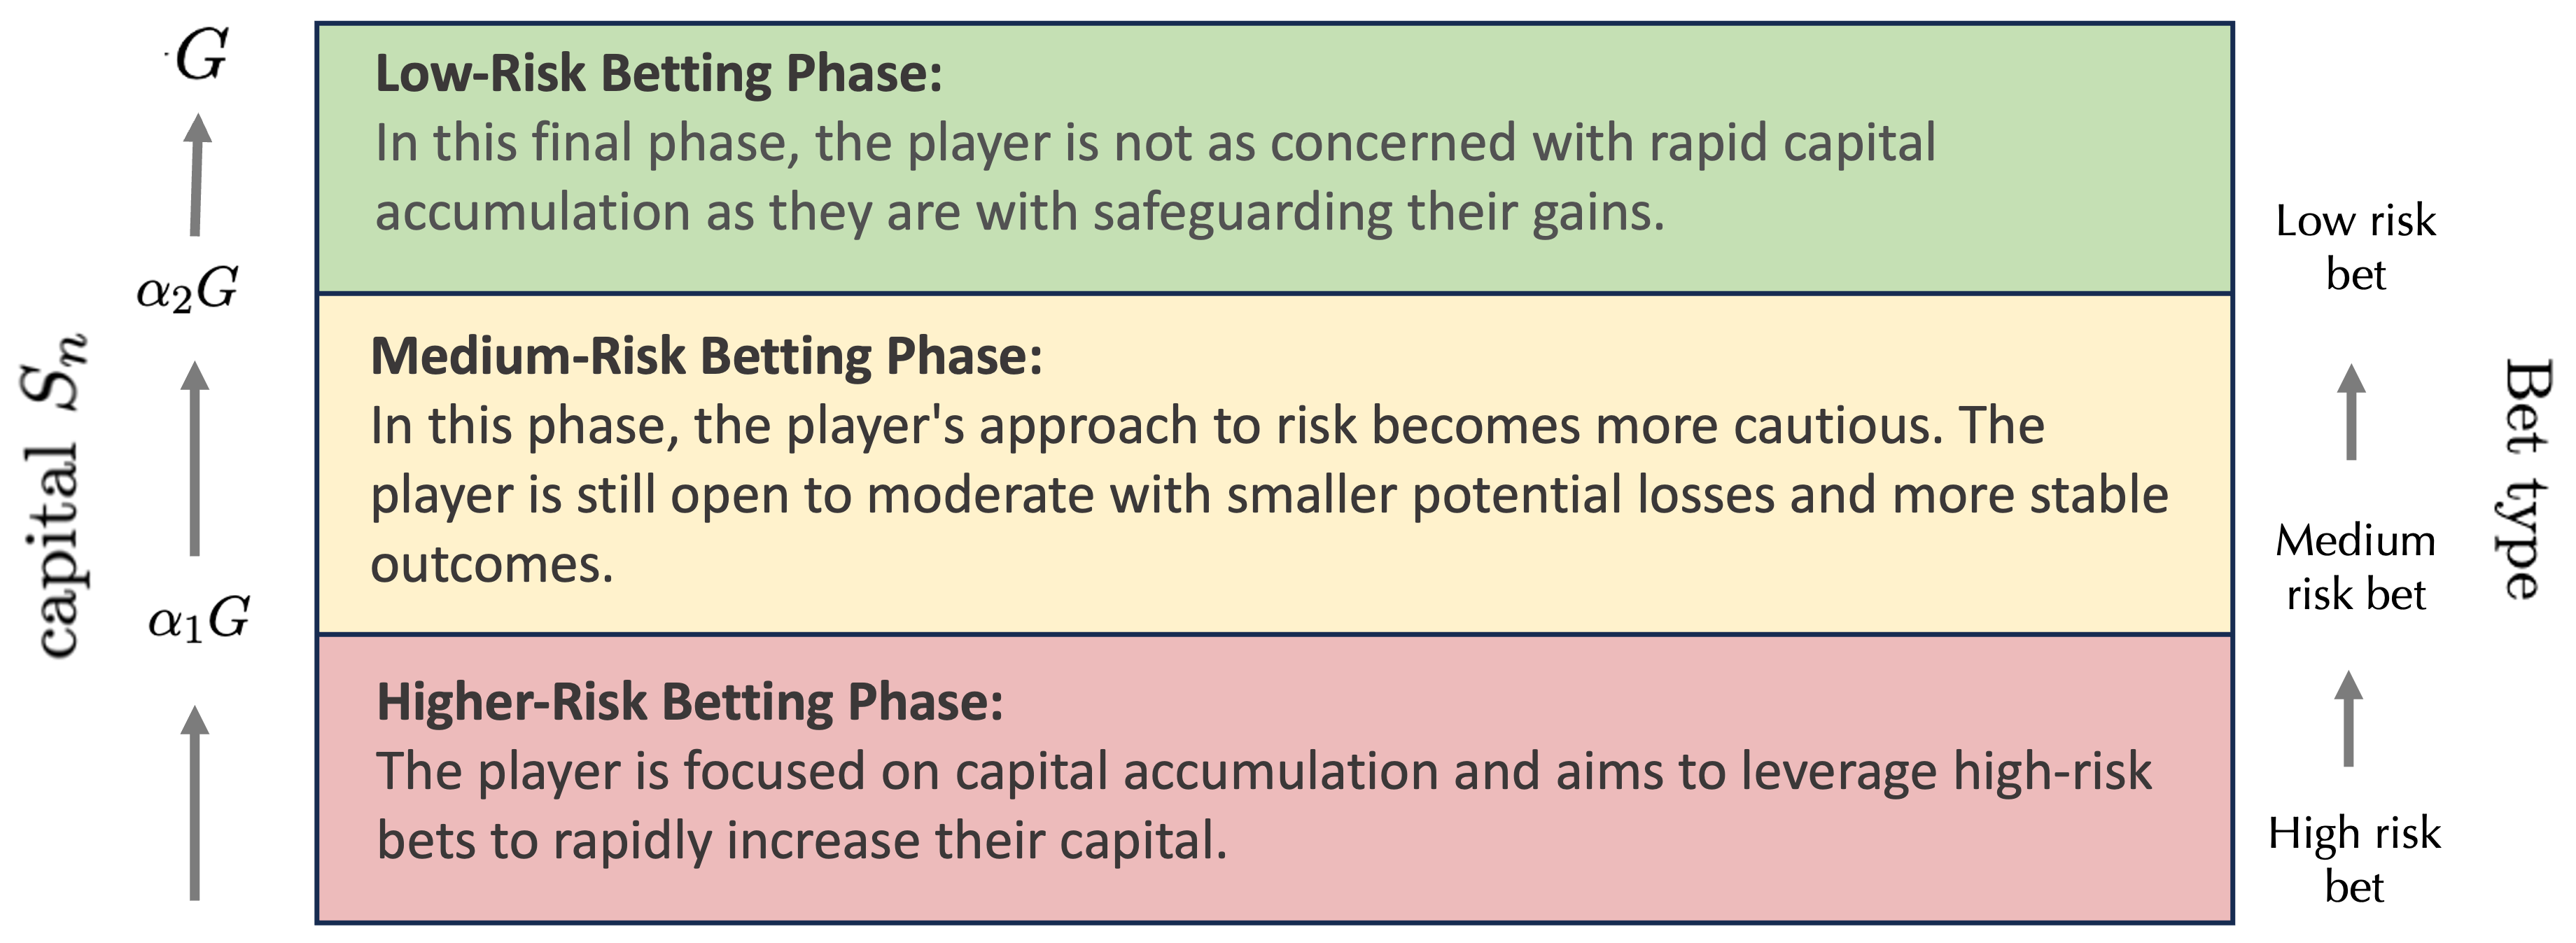
\includegraphics[width=13cm]{mixed.png}
        \caption[Risk adaptable betting phases diagram]{\textit{Risk adaptable betting phases diagram}. Milestones $\alpha_{i}$ define critical points in the player's journey towards their profit goal. They indicate when to switch from risk-taking to risk-averse behaviors.}
\end{figure}

This strategy prioritizes capital preservation and the systematic utilization of different bet types. Simulated scenarios indicate that while the efficacy of this strategy aligns with high-risk strategies, its effectiveness surpasses them; in other words, risk-adaptable strategies may achieve the goal in a shorter time.

In conclusion, the risk adaptable strategy offers a flexible and thoughtful approach to roulette betting, acknowledging the evolving risk appetite of the player. Its combination of proportional betting and strategic transition between bet types makes it a balanced alternative in the pursuit of profit.

\subsection{Report outline}
This report is organized into the following chapters:
In the first part of Chapter \ref{Literature_review}, a comprehensive literature review is presented, discussing the criteria used in previous research to identify optimal betting systems for general chance games. Subsequently, this chapter delves into the most pertinent research concerning the intriguing nature of randomness in the game of roulette, along with an overview of recommended strategies tailored to this specific game.

Chapter \ref{Roulette} provides an overview of the roulette game, detailing its rules, available betting options and payoffs, an examination of its negative expectation, as well as an explanation of the most common misconceptions that may affect the gambler's strategy. Additionally, this chapter presents the test to assess whether a roulette wheel bias is affecting the probability distribution of each number, including an example using real-life information from the Smart Live Casino.
 
Chapter \ref{Gambler} includes the calculation of the probability of ruin and the expected duration of the game for both the classical gambler's ruin problem, centered around even-money payoff bets, as well as its extension to the more general \textit{m-to-1} payoff bets.

Chapter \ref{Betting_systems} presents various betting systems, including the flat betting system, proportional betting system, Martingale betting system, and introduces a novel risk-adaptable betting system. The advantages and disadvantages of each strategy are discussed, and the pseudocode for simulating game paths under each system is provided.

Chapter \ref{Empirical_analysis} includes two separate exercises that were defined to compare the performance of different betting strategies. Also, some examples using the Smart Live Casino data are presented.

Chapter \ref{Conclusions} presents my reflections on this work, as well as the limitations and ideas for future research.

Lastly, the Appendix includes the Smart Live Casino data used throughout the report, along with the corresponding source code employed for simulations and computations.

In this report, I have chosen an approach that begins with a simple example before delving into more complex and generalized concepts. By presenting a straightforward scenario initially, I aim to provide readers with a clear and accessible starting point to understand the fundamental principles of the topic. 

\clearpage
\section{Literature review}\label{Literature_review}
In this chapter, we introduce the concept of favorable games, aiming to comprehend their significance and the rationale behind researchers' inclination towards these games in the context of investigating betting strategies. After that, we outline certain criteria that have guided the identification of optimal strategies for general casino games. Finally, we present the most relevant research works about roulette, along with a presentation of the strategies recommended for this particular game, as documented in the existing literature.

\subsection{Betting systems}
Rational betting, unlike impulsive or emotional betting, aims to identify optimal betting strategies that maximize the expected value of a gambler's utility function. The pursuit of rational betting naturally led to the exploration of whether certain types of chance games are more favorable for players than others. In the literature, games of chance are classified into two categories: favorable and unfavorable. This classification relies on the expected profits that a player can attain within a single round of the game. A game is said to be favorable when the player is expected to make a profit or have a higher average return compared to the amount they wager\cite{Dubins}. Mathematically, it can be expressed as:
\begin{equation}
0 < E(\text{Profit in round }i) = \beta\phi p -\beta(1-p),
\end{equation}\label{expectation_1}
where:
\begin{eqnarray*}
    \beta&:& \text{bet amount,}\\
    \phi&:& \text{payoff of the chosen bet type,}\\
    p&:& \text{probability of winning, and}\\
    q = 1-p &:&  \text{probability of losing}.
\end{eqnarray*}

Another equivalent definition of favorable games is offered by L. Breiman in 1961\cite{Breiman_1961}, defining them as games where $p > \frac{1}{\phi + 1}$. This definition explains the notion that a favorable game provides advantageous odds, offering higher chances of consistent profits.

The definition of favorable games becomes important because a substantial portion of the existing literature has predominantly focused on the analysis of these kinds of games\cite{Kelly, Breiman_1961, Dubins, Ethier_1982, Finkelstein_1981, Smith}. The rationale behind this emphasis lies in the fact that favorable games offer advantageous odds, thereby enhancing the potential for consistent profit generation while concurrently mitigating the associated risk of bankruptcy.

Nevertheless, researchers have adopted diverse criteria to identify optimal betting systems. Some scholars have delved directly into the potential for profit, searching for strategies that maximize the player's initial capital\cite{Thorp} or related indicators, such as long-term growth rates\cite{Kelly}. Other approaches are based on probability analysis. Certain researchers have explored strategies aiming to maximize the likelihood of reaching predefined targets\cite{Breiman_1961, Dubins, Ross_1974}, while others have addressed the challenge of minimizing bankruptcy risk through the evaluation of ruin probabilities\cite{Thorp}. Additionally, some studies have focused on practical considerations and proposed including the expected number of rounds in the game as a criterion to design betting systems\cite{Breiman_1961}, ensuring that the optimal strategy is achievable for the gambler.

\subsubsection{Criterion: Maximizing gambler's expected capital}
Thorp\cite{Thorp} presented an intuitive betting system that aims to maximize the expected value of the capital $S_{n}$ for each round $n$. Since the expected value can be expressed as:
\begin{eqnarray}\label{exp_pq}
E(S_{n}) = E(S_{0} + \sum_{i=1}^{n}\beta_{i}X_{i})=S_{0} + \sum_{i=1}^{n}E(\beta_{i}(X_{i})=S_{0} + \sum_{i=1}^{n}E(\beta_{i})(p-q).
\end{eqnarray}

This equation provides insight into the strategy that maximizes (\ref{exp_pq}):
\begin{itemize}
    \item If $p = \frac{1}{2}$, then $E(\beta_{i})$ does not affect $E(S_{n})$.
    \item If $p > \frac{1}{2}$, then $E(\beta_{i})$ should be maximized, which can be achieved by betting all available capital, $\beta_{i} = S_{i-1}$.
    \item If $p < \frac{1}{2}$, then $E(\beta_{i})$ should be minimized, implying betting the lowest possible amount, $\beta_{i} = 0$.
\end{itemize}

To sum up, the strategy is as follows:

\begin{tcolorbox}[colback=gray!10,boxrule=0.25pt]
\textbf{Strategy that maximizes gambler's expected capital}. \\
\begin{equation*}\label{strategy_1}
\beta_{i} = \left\{
\begin{array}{ll}
S_{i-1}&  p \geq 1/2\\
0 &  p< 1/2.\\
\end{array}
\right.
\end{equation*}
\end{tcolorbox}

This strategy is straightforward and easy to understand, but it proves particularly effective in favorable games where the gambler has a higher probability of winning than losing. In such cases, maximizing bets when the odds are in the gambler's favor helps accelerate capital growth. However, in unfavorable games where the gambler is more likely to lose, the strategy suggests refraining from betting to minimize losses. This aligns with the principle of \textit{if you're not sure you'll win, it's better not to bet}. For cases in which the gambler seeks to achieve a specific profit level or reach a particular goal, this strategy might not be as useful. This is because its focus lies in conservatively maximizing expected capital rather than aiming for higher targets.

\subsubsection{Criterion: Maximizing the capital growth rate}
Another approach used by researchers to construct betting strategies is the Kelly criterion, a well-known formula designed to determine the bet size that maximizes the rate at which a gambler's wealth grows over time. The concept was introduced by J. Kelly in 1956\cite{Kelly} and determines the optimal fraction of capital to bet based on the associated probabilities and payoffs. The Kelly criterion is defined as 
\begin{eqnarray}\label{kelly_crit}
    l^{*} = \frac{\phi p-q}{\phi}.
\end{eqnarray}
Mathematically, the Kelly criterion is the proportion of capital that maximizes the expected value of the logarithm of the gambler's capital growth. A way to deduct this criterion is presented below.

Let's assume the gambler is following a fixed proportional betting strategy that is, the bet amount $\beta_{i}$ 
is the proportion $l$ of the available capital, where $0<l<1$.

For $n$ fixed, the random variables $W_{n}$ and $L_{n}$ denote the number of wins and losses after the $n$ rounds, respectively. Given an initial capital $S_{0}$, we can write the capital after the $n$th round as follows:
\begin{eqnarray*}
    S_{n} = S_{0}(1+l\phi)^{W_{n}}(1-l)^{L_{n}}, & W_{n}+L_{n} = n.
\end{eqnarray*}

Now, let's define the capital geometrical growth rate $r_{n}$:
\begin{eqnarray}\label{capital_growth_rate}
    r_{n}= \left(\frac{S_{n}}{S_{0}}\right)^{1/n} = (1+l\phi)^{W_{n}}(1-l)^{L_{n}}.
\end{eqnarray}

Taking the logarithm and then the expectation in both sides:
\begin{eqnarray*}
E(\log r_{n}) &= &E\left(\frac{W_{n}}{n}\log(1+l\phi)+ \frac{L_{n}}{n}\log(1-l)\right)\\
& = & \log(1+l\phi) E\left(\frac{W_{n}}{n}\right)+ \log(1-l)E\left(\frac{L_{n}}{n}\right)\\
& = & \log (1+l) p + \log(1-l)q.
\end{eqnarray*}

For the last line, we use that \(E(W_{n}) = np\) and \(E(L_{n}) = nq\). To find the value of \(l\) that maximizes (\ref{capital_growth_rate}), let's differentiate the above expression:

\begin{eqnarray}\label{derivative}
\frac{dE(\log r_{n})}{dl}= \frac{p\phi}{1 + l\phi} + \frac{-q}{1 - l}.
\end{eqnarray}

Making (\ref{derivative}) equal to zero, a critical point given by (\ref{kelly_crit}) is found. In fact, $l^{*}$ is a local maximum since
$$\frac{d^{2}E(\log r_{n})}{d l^{2}}\bigg|_{l=l^{*}} =\frac{-p\phi}{(1 + l^{*}\phi)^{2}} + \frac{-q}{(1 - l^{*})^{2}} < 0.$$

Hence, the strategy using the Kelly criterion is as follows: 
\begin{tcolorbox}[colback=gray!10,boxrule=0.25pt]
\textbf{Strategy using the Kelly criterion}. \\
\begin{equation*}
\beta_{i} = \left\{
\begin{array}{ll}
l^{*}S_{i-1}&  l^{*}>0\\
0 &  \text{otherwise},\\
\end{array}
\right.
\end{equation*}\label{strategy_kelly}
\centering
where  $l^{*} = \frac{\phi p-q}{\phi}$.
\end{tcolorbox}

In the long run, the Kelly criterion can help achieve the maximum growth rate of wealth. However, in the short term, it might lead to outcomes that seem counter-intuitive or even risky. This is because the criterion can suggest relatively aggressive bet sizes that might not align with an individual's risk tolerance or the variability of short-term outcomes. In some cases, the recommended bet size might be larger than what a more cautious approach would dictate.

\subsubsection{Criterion: Maximizing the probability of reaching a goal}
For those cases in which the gambler has a profit target $G$, perhaps the most popular strategy is the one defined by Dubins \& Savage\cite{Dubins}, known as the Bold strategy. In such an strategy, the size of the bet is determined based on the current capital of the bettor and the corresponding odds of the type of bet. This strategy aims to maximize the probability of reaching $G$.

It is assumed the gambler starts with an initial fortune $S_{0} =z$ and is allowed to stake any amount of his current capital, that is $0\leq \beta_{i} \leq S_{i-1}$. In the simplest form of this strategy, it is also assumed that the bet type offers a payoff of 1 (even-money payoff), that is if the player wins, the new capital would be $S_{i} = S_{i-1} + \beta_{i}$ or $S_{i} = S_{i-1} - \beta_{i}$ otherwise. In that case, the strategy is as follows:
\begin{tcolorbox}[colback=gray!10,boxrule=0.25pt]
\textbf{Bold strategy for even-money payoff case}.\\
\begin{equation*}\label{strategy_bold}
\beta_{i} = \left\{
\begin{array}{ll}
S_{i-1}&  S_{i-1} \leq G/2\\
S_{i-1}\left( 1  - \frac{S_{i-1}}{G}\right) & otherwise.
\end{array}
\right.
\end{equation*}
\end{tcolorbox}

In essence, this strategy involves placing the largest possible bet that, if won, would not exceed the profit target. Dubins and Savage demonstrated that the Bold strategy remains optimal even if the game is unfavorable for the gambler ($p \leq \frac{1}{\phi + 1}$).

The Bold strategy marked the inception of a general theory for gambling problems and stands as one of the most significant contributions by Dubins and Savage. This recognition is justified by their early pioneering work\footnote{Although their most cited book wasn't published until 1965, their foundational work dates back to 1956, as noted by \cite{Breiman_1961}.}. While the Bold strategy is arguably the most frequently referenced outcome in this context, its optimality does not always endure when extensions seek to generalize or incorporate more realistic aspects\cite{Yao, Wilkins}. For instance, when constraints are introduced to limit the number of rounds in the game, the Bold strategy remains optimal where $p \leq \frac{1}{\phi + 1} = 1/2 $ and $1/2 = p \leq \frac{1}{\phi + 1}$. However, the general optimality of this strategy is not retained when such limiting conditions are applied. Moreover, J. Schweinsberg\cite{Schweinsberg_2005} examined a scenario where the gambler is constrained by casino-imposed limitations that restrict their bets to a proportion $\delta$ at a time. In this study, it was demonstrated that the Bold system is not optimal when the value of $\delta$ is irrational.
\subsubsection{Criterion: Minimizing ruin probability}
Thorp\cite{Thorp} presents a range of betting strategies designed to minimize the probability of ruin, where ruin is understood to occur after the $j$th outcome if $S_{j} = 0$. One of the strategies is the following:
\begin{tcolorbox}[colback=gray!10,boxrule=0.25pt]
\textbf{Halving Strategy}.\\
\begin{equation*}
\beta_{i} = S_{i-1}/2.
\end{equation*}
\end{tcolorbox}

Under this strategy, the gambler bets always a half of their available capital, which limits the potential loss in the event of a losing outcome. This approach is designed to reduce the impact of consecutive losses and the probability of reaching a point where the gambler's capital is completely depleted (bankruptcy).

Another strategy that prevents bankruptcy is the following: 
Let be $r$ a positive rational number such that $Gr$ and $rS_{0}$ are integers. 

\begin{tcolorbox}[colback=gray!10,boxrule=0.25pt]
\textbf{Rational bet Strategy}.\\
\begin{equation*}
\beta_{i} = \left\{
\begin{array}{ll}
1/r&  0 < S_{j-1} < G\\
0 &  S_{j-1} \leq 0 \text{ or }S_{j-1} \geq G.\\
\end{array}
\right.
\end{equation*}
\end{tcolorbox}

This strategy is equivalent to bet $1$ when the initial capital and the goal are the integers $zr$ and $Gr$, respectively. Let  $R(r)$ the probability of ruin, then by the gambler's ruin analysis:
\begin{eqnarray*}
R(r)  = \frac{\theta^{Gr} - \theta^{S_{0}r}}{\theta^{Gr} -1}, & \text{ where } p\neq 1/2 \text{ and } \theta = q/p.
\end{eqnarray*}

\begin{itemize}
    \item If $1> p > 1/2$, $R(r)$ is an strictly decreasing function of $r$. 
    \item If $0< p < 1/2$, $R(r)$ is an strictly increasing function of r. 
\end{itemize}
Since $0\leq R(r) \leq 1$, it is not hard to see that when $p>1/2$ then $\theta < 1$ and
\begin{eqnarray*}
    \lim_{r \to \infty} R(r) =  \lim_{r \to \infty}\frac{\theta^{Gr}- \theta^{S_{0}r}}{\theta^{Gr} -1} = 0.
\end{eqnarray*}
Hence, making sufficient small bets $1/r$, the probability of ruin become arbitrarily small. \\

While these two strategies are effective at preventing bankruptcy and ensuring that the gambler can continue playing for an extended period, they also come with considerable limitations. These strategies might not be appealing to gamblers seeking rapid growth or aiming to reach specific profit targets quickly. Furthermore, many casinos and gambling platforms impose minimum wager limits, potentially rendering these strategies infeasible in the long-term.

Another betting system designed for minimizing ruin probability is known as the Timid strategy\cite{Thorp, Ross_1974}:
\begin{tcolorbox}[colback=gray!10,boxrule=0.25pt]
\textbf{Timid Strategy}.\\
\begin{equation*} \label{strategy_timid}
\beta_{i} = \left\{
\begin{array}{ll}
1&  1 \leq S_{j-1} \leq G-1\\
0 &  \text{ otherwise}.\\
\end{array}
\right.
\end{equation*}
\end{tcolorbox}

This system minimizes the probability of ruin among strategies where $\beta_{i}$ is an integer, satisfying $1 \leq \beta_{i} \leq \min\{S_{0}, G-S_{0}\}$. This result is not difficult to understand, as betting one unit at a time maximally extends the duration of the game while limiting the amount at risk. Consequently, this strategy also maximizes the time until the bettor goes bankrupt when $p \geq 1/2$.

While this strategy reduces the likelihood of losing all the capital, it might also limit potential gains if the corresponding payoff is small. Based on these three examples of strategies that minimize the risk of bankruptcy, it becomes evident that the most straightforward way to prevent bankruptcy is to avoid betting large amounts of money each round. However, this cautious approach often results in unremarkable profits. Thorp\cite[PP.284]{Thorp} concludes about this kind of strategies as follows:
 \begin{quote} 
{\fontfamily{qpl}\selectfont
The strategy which minimizes ruin has the unsatisfactory consequence that it also minimizes our expected gain. Some strategy is called for which is intermediate between minimizing ruin (and expectation) and maximizing expectation (and assuring ruin).}
\end{quote}

\subsubsection{Criterion: Minimizing the expected number of rounds}
Another criterion for finding optimal betting strategies, described by Breiman \cite{Breiman_1961}, focuses on finding a gambling strategy that minimizes the expected number of trials needed to win or exceed the target amount $G$. In other words, this approach try to find a strategy to reach the profit target in the shortest possible time, on average.

Let's suppose the gambler have fixed the number of rounds he is going to bet, let's say $N$. The aim of this approach is to find a strategy which maximizes the following probability:
\begin{equation}
    P(S_{N} \geq G \text{\textbar} S_{0} = z).
\end{equation}
The author worked with the equivalent problem of maximizing 
$P(S_{N} \geq 1 \text{\textbar} S_{0} = z/G)$ and found that for $p > 1/2$, the optimal strategy is to bet a fraction $p - q$ of the available capital in each round. This result coincides with the Kelly strategy with $\phi=1$. Once again, the main results are applicable to favorable games.

\subsection{Exploring the Roulette case}
The exploration of the physics and mechanics behind the roulette wheel to understand the randomness of the game has been a subject of interest for various researchers, including Poincaré, Pearson, and Thorp. Poincaré studied the angular position and velocity of the ball and rotor at a given time. He discovered that under specific conditions, the roulette wheel can exhibit behavior that closely resembles a random process, despite being governed by deterministic laws of physics\footnote{In his book \textit{The Perfect Bet: How Science and Maths are taking the luck out of gambling}, Adam Kucharski wrote: “As Poincaré saw it, events like roulette appear random because we are ignorant of what causes them”.}. 

In 1894, Karl Pearson suggested that despite a roulette wheel being meticulously designed and regularly maintained, it may not always behave as expected based on the laws of probability. With this idea in mind, Pearson developed a test\cite{Agresti}, known as Pearson's chi-squared test, to measure the discrepancy between the observed and expected frequencies in a multinomial experiment. This test proved valuable in identifying potential biases or irregularities in roulette outcomes by comparing actual data to theoretical expectations.

Thorp's research\cite{Thorp}, on the other hand, focused on predicting winning numbers by analyzing the initial position and velocity of the ball and rotor. However, he encountered additional sources of randomness in the system that were not fully understood, leading to results that lacked complete reliability. A notable finding in his study was the impact of a slight tilt in the roulette wheel. Even a minimum bias of just 0.2° could cause the ball to avoid falling into a particular sector of the track on the “high” side. This effect was particularly pronounced, creating a forbidden zone that spanned approximately a quarter to a third of the wheel, where the ball was less likely to land due to the tilt.

In addition to investigating the underlying physics and mechanics of the roulette wheel, researchers have tried to find an optimal strategy for the game. Already mentioned Dubins and Savage \cite{Dubins} stated the problem of determining the optimal betting strategy for the roulette game with the objective of maximizing the probability of achieving a specific target $G$ starting with a small initial capital. The optimal strategy found can be understood as a general bold strategy which considers the \textit{uniform roulette} condition. Under that condition, bettors can place bets on multiple numbers simultaneously, but with the requirement that the exact same amount of money must be wagered on each of the selected numbers. 
Considering a general $\phi$ payoff bet where $\phi$ is a positive integers, the optimal strategy is as follows:

 \begin{tcolorbox}[colback=gray!10,boxrule=0.25pt]
\textbf{Bold strategy for $\phi$ payoff case}.\\
\begin{equation*}
\beta_{i} = \left\{
\begin{array}{ll}
 S_{i-1}&  S_{i-1} \leq \frac{G}{\phi+1}\\
\frac{G-S_{i-1}}{\phi} & otherwise.
\end{array}
\right.
\end{equation*}
\end{tcolorbox}

If at round $i$ the available capital is less than $G/(\phi+1)$, the player places his entire fortune on a single bet with payoff $\phi$. Otherwise, if the current fortune $S_{i-1}$ is greater than $G/(\phi+1)$, the gambler bet in the next bet the exact amount of money so that after multiplying by the payoff in case of winning, the player reaches his goal.

Smith\cite{Smith} extended the result and stated that bold strategy is also optimal when no restrictions on the relative sizes of bets on various numbers are imposed, that is, the \textit{uniform roulette} condition can be relaxed.

Martinez et.al.\cite{martínez2016} analyzed data from a real network casino in Riga, Latvia. They modeled the probabilities of occurrence of the numbers using Ornstein-Uhlenbeck processes and then evaluated the effectiveness of different betting systems in the short term by simulating scenarios. One of the systems they examined was the strategy generated using the Kelly criterion. However, when applied to an unfavorable game like roulette, the Kelly Criterion does not yield a useful betting amount. For instance, let's consider a roulette bet on a single number. In this case, the calculated optimal betting proportion is approximately $-0.027$, which is negative. The negative value indicates the gambler not to bet on a single number in roulette, as the expected outcome is a net loss. Similar advice is given when betting on a specific color, any dozen, or in general any bet types offered in roulette due to the house edge inherent in the game. Thus, in all these cases, the Kelly Criterion suggests betting a proportion of capital that would ultimately lead to an overall loss in the long run. It becomes evident that the Kelly Criterion may not be suitable for optimizing bets in unfavorable games.


\clearpage
\section{Roulette} \label{Roulette}
\subsection{Background}
Roulette is a popular casino game. Its origins trace back to a combination of a gaming wheel and an Italian game called \textit{Bijibi}. The game gained immediate popularity in Paris, particularly among the upper classes and later spread its popularity across the globe, where different versions of the game were innovated. The most significant and widely recognized versions are the European and the American roulette\footnote{There are other variations such as French roulette, mini roulette, double ball roulette, among others.}.

The game is played on a specialized table with a spinning wheel that is divided into numbered compartments. In the European version, there are 37 compartments, numbered 1 to 36, with a single zero (0), while in American roulette, there are 38 compartments, numbered 1 to 36, with an additional single zero (0) and the double zero (00). Each compartment is colored either red or black, except for the zero(s), which are usually green. The objective of the players is to predict and bet on which numbered pocket the small ball will land in once the wheel stops spinning.

\begin{figure}[ht]
        \centering
        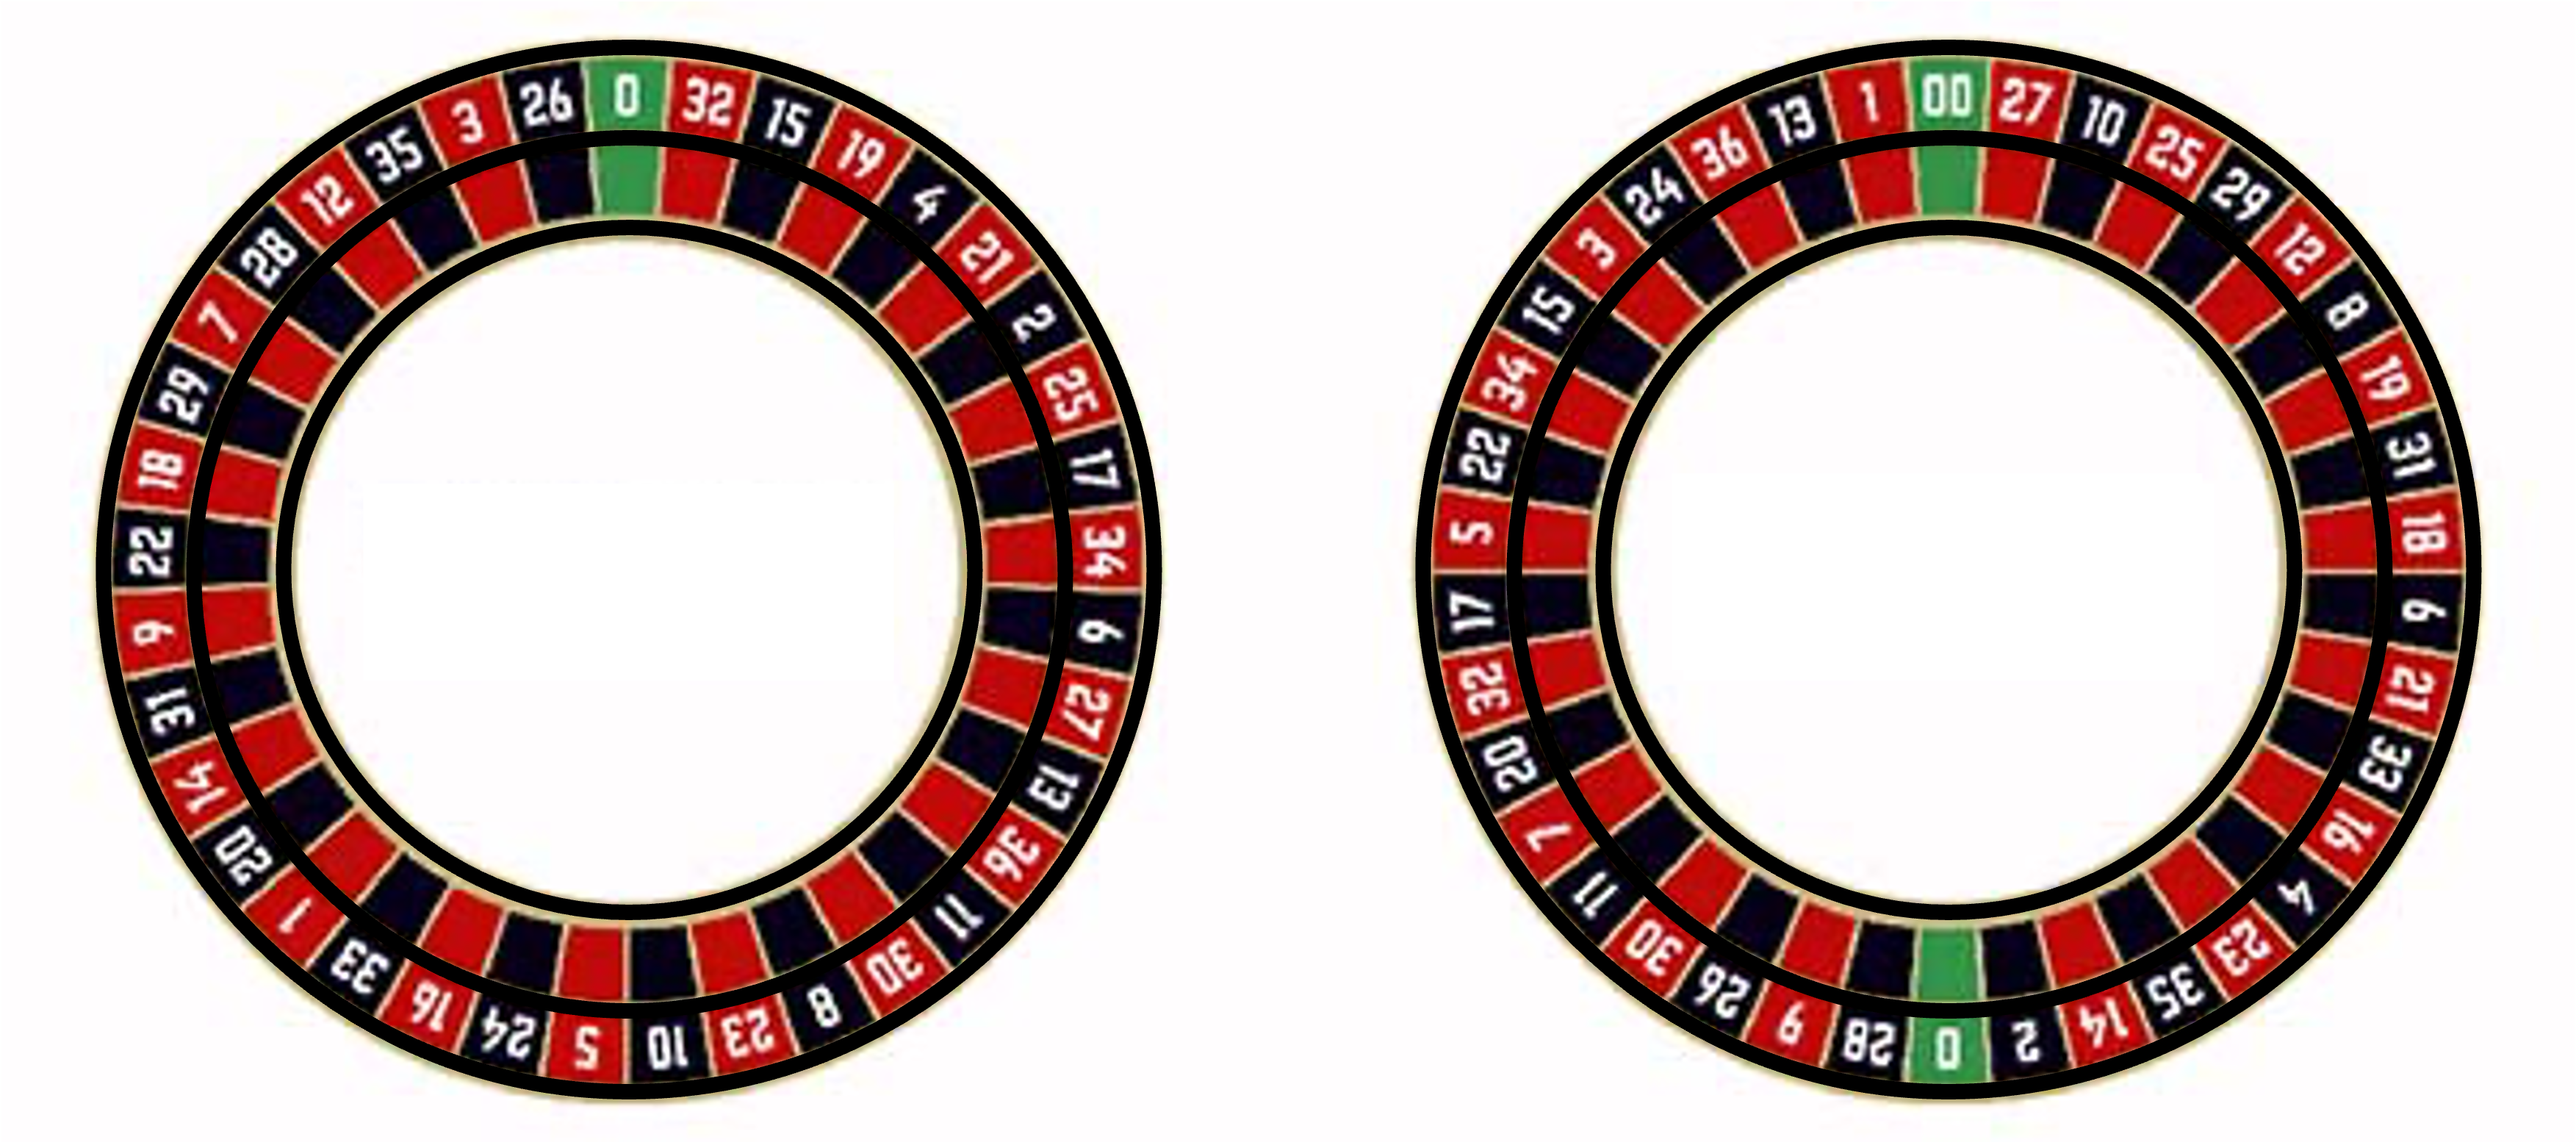
\includegraphics[width=14cm]{wheels.png}
        \caption[American and European Roulettes]{\textit{American and European Roulettes}. The order of the numbers on the American Roulette (right-hand side) is slightly different from the European version (left-hand side), and the additional double zero (00) pocket is located opposite the single zero (0).}
       
\end{figure}

The roulette table also has a designated betting area known as the layout or layout table:
\begin{figure}[ht]
\centering
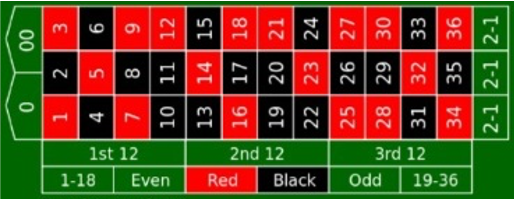
\includegraphics[width=8cm]{layout.png}
\caption[American roulette layout]{\textit{American Roulette layout}. }
\end{figure}

The following is a description of the game mechanism:
\begin{itemize}
\item Setting bets: At the beginning of a round, players place their bets by putting chips\footnote{Instead of directly betting with cash, players exchange their money for chips. Nevertheless, in this dissertation, chips and money are understood to be the same.} on the table layout, which represents the different betting options (see Table \ref{bet_types}). Players can choose to bet on single numbers, groups of numbers, colors (red or black), and more. Multiple bets per gambler are usually allowed.
\item The spin: Once all bets are placed, the casino employee, known as the croupier, spins the wheel in one direction while simultaneously rolling a small ball in the opposite direction along the edge of the wheel. As the ball loses momentum, it comes to rest in one of the numbered compartments, determining the winning number for that round.
\item Payouts: The croupier announces the winning number and pays out the winning bets.
\end{itemize}

The potential payout are defined using the odds or probability of winning. For example, a bet on a single number in the European roulette has odds of 35 to 1, which means the payout is 35 times the bet amount. However, the probability of winning that bet is 1/37 since there are 37 possible outcomes. Bets with higher odds are less likely to win, but the payout would be larger. Conversely, bets with lower odds, such as betting on red or black, have higher probabilities of winning but offer lower payouts. 
\begin{table}[!ht]
\centering
\caption{Different types of bets offered by the European roulette layout}
\begin{tabular}{|c|l|c|}
\hline
Bet type & Description & Payoff\\
\hline\hline
Single & one single number & 35 to 1\\
Split  & two vertically/horizontally adjacent numbers & 17 to 1\\
Street & three consecutive numbers in a horizontal line & 11 to 1\\
Square & four numbers that meet at one corner & 8 to 1\\
Six Line/Double Street & six consecutive numbers that form two horizontal lines & 5 to 1\\
Column &  one of the vertical columns of 12 numbers & 2 to 1\\
Dozen & the first (1-12),  second (13-24), or third (25-36) dozen &2 to 1\\
Red or Black & red or black number subsets& 1 to 1\\
Odd or Even & odd or even number subsets & 1 to 1\\
High or Low & low range (1-18) or high range (19-36) & 1 to 1\\
\hline
\end{tabular}
\label{bet_types}
\end{table}

\subsection{House advantage and negative expectation}
The house advantage refers to the statistical edge that the casino has over the players.  It represents the average percentage of each bet that the casino expects to keep as profit in the long run. When a casino game is designed, a mathematical advantage is built in to ensure the casino makes money over time. In general, game's rules, odds, and payout structure are ways to incorporate the house advantage.   

In the roulette case, the presence of the (0) and (00) (in the American version) represents the house advantage since it bias the odds slightly in favor of the casino. For example,  when placing a 'Red or Black' bet on an European roulette, there are 18 out of 37 possible outcomes that will result in a win. The probability of winning is $18/37 = 0.486$ slightly less than $0.5$. However, the payout associated to this bet was calculated assuming a probability of winning of $0.5$. This discrepancy between the odds and payouts is how the house maintains its advantage over the players in the long run.

Let $\beta_{i}$ be the bet amount in the $i$th round of the game. Let's assume the gambler decides to bet on $j$th bet type with corresponding payoff ($\phi_j$). The expected revenue for the gambler in that round is given by:
\begin{eqnarray}
E(X_{i}) = -\beta_{i}q + \beta_{i} \phi_{j} p  = \beta_{i} (\phi_{j} p - q), \label{expected_value}
\end{eqnarray}

where $p$ and $q$ represents the probabilities of winning and losing when betting on the $j$th bet type.

Applying this formula to the payoffs presented for the European Roulette in Table \ref{bet_types}, the expected value of the gambler's revenue in the $i$th round is:
\begin{eqnarray*}
    E(X_{i}) =  -\frac{1}{37}b_{i}. 
\end{eqnarray*}
It is important to note that the expected value of the gambler's revenue is the same regardless the bet type he chooses. 

The gambler has a negative expected value that corresponds to the (0) compartment. On average, the casino wins $\frac{1}{37}$ times the bet amount per round.

Considering the American roulette, the expectation is drops to $-\frac{2}{38}b_{i}$, meaning that, on average, players are expected to lose about 5.26\% of their bet amount on each wager. 

The Law of Large Numbers ensures that as a player makes a large number of bets, the actual results will tend to converge to the expected value. In other words, as a player makes more and more bets, their actual losses will tend to align with the negative expectation of their bets. This means that, over the long run, players are likely to fall behind and stay behind, losing money at a rate close to the expectation of their bets.
Despite the inherent unfavorable odds, certain individuals are compelled to partake in games such as roulette due to their pursuit of short-term financial gains. The emotional appeal of such short-term earnings, together with the thrill of unpredictability, supersedes rational decision-making, impelling individuals to engage in these games.

When observing a roulette game, it is possible for one particular outcome, such as a specific number or color, to occur more frequently or less frequently than expected over a certain number of spins. In such cases, two possibilities should be considered: the roulette wheel might be biased or unbiased. A biased wheel could result in non-random outcomes due to mechanical imperfections or wear, leading to certain numbers or colors appearing more frequently. Conversely, an unbiased wheel follows the laws of probability, and such variations in outcomes are merely natural fluctuations. To determine whether the roulette wheel is biased or not, a statistical test is necessary, which involves analyzing a significant number of spins to assess if there is a systematic deviation from randomness. However, it is crucial to note that some gamblers mistakenly fall into the trap of the gambler's fallacy, believing that such variations indicate a predictable pattern. In reality, each spin of the roulette wheel is an independent event, and past outcomes do not influence future results, making the gambler's fallacy a misleading belief in the context of random chance games.

\subsection{Misconceptions while betting}

The gambler's fallacy is a mistaken belief that previous outcomes can influence future results in a game of pure chance. It is the idea that if a particular outcome, such as a specific number or color, has occurred more frequently or less frequently than expected in recent spins, then it is “due” to happen or less likely to happen in subsequent spins. For example, let's consider betting on a single number in roulette. Each spin of the roulette wheel is independent, and the probability of any specific number appearing on a single spin $1/37$ remains constant for every spin, regardless of past results. However, the gambler's fallacy can manifest in two ways:
\begin{enumerate}
    \item When a player believes that a particular number is “hot” because it has appeared multiple times in recent spins. They may think that the number is more likely to not appear again in the next spin because all the numbers.
    \item When a number is “cold” because it has not appeared in several spins, a mistaken gambler could think that it's “due” to come up soon. 
\end{enumerate}

In both cases, the players mistakenly assign patterns or significance to random events, falling prey to the gambler's fallacy and overlooking the true nature of probability in games of chance.

At the end of a day in the casino, due to the Law of Large Numbers, we can expect to see more or less the same proportion of each number appearing on the roulette wheel. This fact might seem to lend credence to the gambler's fallacy, as players may observe that the numbers have, on average, appeared with roughly equal frequency. Consequently, some might interpret this statistical equilibrium as an indication that certain numbers are “overdue” or “hot” and are more likely to come up in subsequent rounds. However, this is a misunderstanding of probability and the nature of random events. 

Nevertheless, if a player observes that a particular number appears more frequently than other numbers over a significant number of spins, it would be natural for them to suspect that the roulette might not be entirely unbiased. In such a scenario, the player's suspicion would be reasonable, as it could indicate a potential bias in the roulette wheel.

\subsection{Unbiased wheel assumption}
In a casino, the roulette wheel should be completely fair. This means that all the numbers from 0 to 36 (European roulette) have an equal chance of winning (each with a probability of $1/37$). However, sometimes the roulette wheel is not perfect. It might have some problems that cause certain numbers to win more often than they should. These issues could be due to how the wheel was made or because it has been used a lot.

When probabilities of winning for each number deviate from the expected $1/37$, the wheel is said to be biased. In this case, some numbers might have a slightly higher chance of winning, while others have a slightly lower chance. In contrast, when any number is equally likely to occur, the wheel (or the roulette) is said to be unbiased.

A biased roulette can have a significant impact on the expected revenue of a gambler. Observant gamblers who notice these patterns and exploit them by consistently betting on the numbers with higher observed frequencies may have an advantage. \cite{Ethier_1982} mentioned three documented cases where individuals won significant amounts of money by betting on numbers with the highest observed frequencies in roulette. Nevertheless, those cases occurred between late 19 century and early 20th century so it is not clear to what extent biased roulettes exist in today's casinos. 

Pearson's chi-squared test measures the discrepancy between the observed and expected frequencies in a multinomial experiment\cite{Agresti}. It is particularly useful for identifying whether a roulette wheel is biased or not.

Before introducing Pearson's test, it's important to understand what a multinomial experiment is and why the roulette can serve as an example of such an experiment. A multinomial random variable is a generalization of the binomial random variable that accommodates more than two possible outcomes. The formal definition of a multinomial experiment is as follows:

\begin{Definition}
A multinomial experiment consists of conducting a series of $n$ identical and independent trials, where each trial can result in one of $c$ mutually exclusive categories. Let $y_{ij} = 1$ if trial $i$ results in category $j$, and $y_{ij} = 0$ otherwise. 
\begin{itemize}
    \item The variables $y_{i} = (y_{i1},y_{i2},...,y_{ic})$ represents the outcomes of the multinomial trial $i$,
    \item $n_{j}= \sum_{i}^{n}y_{ij}$ denotes  the  number  of  trials  that result in category $j$,
    \item $(n_{1},...,n_{c})$ is said to have multinomial distribution with parameters $(\pi_{1},...,\pi_{c})$ where:
    $\pi_{j}=P(y_{ij}= 1)$ denotes  the  probability  of  outcome  in  category $j$ for each trial and $\sum_{j=1}^{c}\pi_{j} = 1$. 
\end{itemize}

\end{Definition}
By understanding the concept of a multinomial experiment, it is not hard to see the frequencies of each number appearing after $n$ spins of the roulette follow a multinomial distribution. In each roulette spin, there are multiple possible outcomes, each corresponding to a specific number on the wheel. For example, in European roulette, there are 37 categories, while the American version has 38 categories. After observing a series of $n$ roulette spins, we obtain the values of $n_{j}$, representing the number of times each category $j$ appears. From these observations, we can estimate the probabilities $\pi_{j}$ using $\hat{\pi}_{j}= n_{j}/n$.

Then, the following test hypotheses can be defined:
\begin{align*}
H_{0}: \pi_{1}= \pi_{2}= \ldots = \pi_{c} = \frac{1}{c},\\
H_{1}: \pi_{i} \neq \frac{1}{c} \text{ for some }i \in \{1, \ldots, c\}.
\end{align*}

The null hypothesis ($H_{0}$) assumes that all categories are equally likely, meaning the roulette wheel is unbiased. Conversely, the alternative hypothesis ($H_{1}$) suggests that the wheel is biased, and at least one of the probabilities $\pi_{i}$ is not equal to $1/c$. When the null hypothesis is true, the expected values (or expected frequencies) for each category are $n/c$.

\begin{Definition}
The Pearson's chi-squared statistic test is defined as:
\begin{eqnarray}
\chi_{o}^2 = \sum_{i=1}^{c}\frac{(n_{i} - n/c)^2}{n/c},
\end{eqnarray}
where $n_{i}$ represents the observed frequencies of each category, and $n/c$ denotes the expected frequencies in $n$ observations, assuming the null hypothesis is true.
\end{Definition}

For a fixed $n$, greater differences ($n_{i} - n/c$) between observed and expected frequencies result in larger $\chi_{o}^2 $ values. In the case of large samples, the $\chi^2 $ statistic approximately follows a chi-squared distribution with $c-1$ degrees of freedom\cite{Agresti}. The $p$-value of this test can be approximated by $P(\chi_{c-1}^2 \geq \chi_{o}^2)$. Finally, if the p-value is smaller than the chosen significance level ($\alpha$), typically 0.05 or 0.01, then the null hypothesis ($H_{0}$) is rejected in favor of the alternative hypothesis ($H_{1}$).

Let's suppose that at a given significance level $\alpha$, the test determined that the roulette wheel is biased, the next step is identify the specific compartments that might be biased. In that case, it is needed calculate the Chi-squared contribution for each compartment:
\begin{eqnarray*}
    \chi_{o,i}^2 = \frac{(n_{i} - n/c)^2}{n/c}, & \text{for }i = 1,...,c.
\end{eqnarray*}

Then, using the Chi-squared contributions calculate the p-value associated with each compartment by computing $P(\chi_{1}^2 \geq \chi_{o,i}^2)$, where $\chi_{1}$ is a random variable that follows a chi-squared distribution with 1 degree of freedom. This $p$-value represents the probability of observing deviations as extreme as those in the data, assuming no bias.

Comparing the calculated $p$-value for each compartment with a chosen significance level $\alpha$ will determine if the observed deviations for that compartment are statistically significant. If the p-value for a compartment is less than $\alpha$, that specific compartment is significantly biased, otherwise there is not enough evidence to conclude that the observed deviations for that compartment are statistically significant.

Additionally, it is worth noting that the same principles and tests can be applied to different categories within the context of the roulette. The player with historical information can test whether neighborhoods or subsets of compartments exhibits a higher probability than expected. This approach enables discerning whether a specific color, dozen, square, or other grouping is statistically more likely to emerge as the winning subset, providing valuable insights for strategic betting decisions.
 
Let's suppose a scenario where only one compartment of the wheel is biased, and let's assume the gambler has noticed such a bias and decided to bet on the number corresponding to that compartment. We can determine the size of the bias that would transform the game from a negative expectation to a positive one by using the expression (\ref{expected_value}) for the expected value of the gambler's revenue:
\begin{eqnarray}
0 < E(X_{i}) -\beta_{i}q +35\beta_{i}p & \text{ if and only if }& p > 1/36.
\end{eqnarray}

When a compartment has positive bias greater or equal to $(1/36 - 1/37)$ the game will have a positive expectation for the gambler. The implications of such a bias would allow the player to use all the betting systems presented in the Chapter \ref{Literature_review} that are valid for favorable games.

\subsubsection{Example using real life data}
To investigate the presence of bias in a roulette, real-life data from 5,550 roulette spins in the Smart Live Casino in UK were collected. The raw information corresponding to January 2011 was obtained grouped into images each of those containing 185 roulette spin outcomes. The data was collected from \url{www.RouletteForum.cc}, a platform where users share real roulette spin numbers for testing accuracy and predicting winning numbers.

The outcome numbers were extracted from the images using Google Translate's Optical Character Recognition (OCR). This process converted the text in the images into machine-readable data. The extracted outcome numbers were saved into an Excel file. To ensure the accuracy and reliability of the extracted data, a manual cross-check was performed for each extracted number in the Excel file against the original numbers in the images.

The complete data set of 5,550 roulette spins from the Smart Live Casino in the UK can be found in Table \ref{tab:casino_data} in the Appendix.

The observed frequencies ($n_{j}$) of the roulette ball landing on each number during the $n$ spins were computed. Also, the estimated probabilities ($\hat\pi_{j}$) to observe each number in the roulette were calculated. The resulting frequencies and probabilities are summarized in Table \ref{tab:freq_prob}.

\begin{table}[htbp]
  \centering
  \caption{Smart Live Casino data summary}
  \label{tab:freq_prob}
  \begin{tabular}{|ccc||ccc|}
    \hline
    \textbf{Number} & \textbf{Frequency} & \textbf{Probability} & \textbf{Number} & \textbf{Frequency} & \textbf{Probability} \\
         & \textbf{($n_{j}$)} & \textbf{($\hat\pi_{j}$)} &  & \textbf{($n_{j}$)} & \textbf{($\hat\pi_{j}$)} \\
    \hline
0&146&0.026&19&156&0.028\\
1&154&0.028&20&156&0.028\\
2&164&0.030&21&164&0.030\\
3&137&0.025&22&146&0.026\\
4&120&0.022&23&162&0.029\\
5&148&0.027&24&143&0.026\\
6&142&0.026&25&145&0.026\\
7&148&0.027&26&157&0.028\\
8&155&0.028&27&149&0.027\\
9&177&0.032&28&148&0.027\\
10&151&0.027&29&172&0.031\\
11&138&0.025&30&142&0.026\\
12&161&0.029&31&145&0.026\\
13&149&0.027&32&142&0.026\\
14&158&0.028&33&146&0.026\\
15&142&0.026&34&158&0.028\\
16&139&0.025&35&135&0.024\\
17&166&0.030&36&161&0.029\\
18&128&0.023&&&\\
\hline
  \end{tabular}
\end{table}

The most repeated numbers were 9 and 29, while the number 4 was the least popular. To test the bias of the roulette wheel, the chi-squared test was conducted. The null hypothesis ($H_{0}$) states that all numbers are equally likely, indicating an unbiased wheel. The alternative hypothesis ($H_{1}$) suggests that the wheel is biased, with at least one number having a different probability.
\begin{align*}
H_{0}: \pi_{1}= \pi_{2}= \ldots = \pi_{37} = \frac{1}{37},\\
H_{1}: \pi_{i} \neq \frac{1}{37} \text{ for some }i \in {1, \ldots, 37}.
\end{align*}
The Pearson's chi-squared statistic test was applied to the observed frequencies ($n_{j}$) and expected frequencies. The latter are equal to $5,550/37 = 150$.

\begin{equation}
\chi_{o}^2 = \sum_{i=1}^{37}\frac{(n_{i} - 150)^2}{150} = 192.5 \notag
\end{equation}

The computed $\chi_{o}^2 = 192.5$ value was then compared to the critical value from the chi-squared distribution with $36$ degrees of freedom. Thus, the estimated $p$-value of the test computed as $P(\chi_{36}^2 \geq 192.5)$ is equal to 0.597. Following the decision rule, the null hypothesis ($H_{0}$) cannot be rejected using a 95\% confidence level. Therefore, there was no significant evidence of bias in the wheel, indicating that the observed frequencies closely matched the expected frequencies based on an unbiased wheel.

\section{Gambler's ruin problem}\label{Gambler}
\subsection{Background}
The gambler's ruin problem is a concept in probability and gambling theory that examines the risk of losing all gambling capital or going bankrupt and it is used to analyze the long-term results of a gaming session. The original statement of this problem was focused on calculating the probability of ruin of a gambler playing with three dice and came from a letter written by Blaise Pascal to Pierre Fermat in 1656. Both mathematicians solved this problem independently and apparently with different methods. Later, the contributions of many others, such as Abraham De Moivre and Nicolaus Bernoulli, also made it possible to know the estimated duration of the game before the ruin. More detailed notes on the history of the gambler's ruin problem can be found in \cite{chances, history}.


The discrete-time Markov chain (DTMC) theory allows for a comprehensive analysis of various aspects of the Gambler's ruin problem, such as the probability of ruin, expected duration of the game, and the likelihood of reaching specific profit targets.


\subsection{Even-money payoff case or classical problem}
In the simplest form of the problem, two players participate in a series of repeated bets. Each player starts with a certain integer amount of money and continues to place 1-unit bets until one of them loses all of his capital. 

Usually one of the player is denoted as \textit{the gambler} and the other as \textit{the house}. This characterization comes along with certain assumptions about their respective capitals and the probabilities of winning. The gambler typically represents an individual player who has a finite amount of capital while the house refers to the entity running the gambling operation, such as a casino or a lottery organizer, which generally has a larger capital and had defined the rules of the game. In terms of probabilities, the house is assumed to have an advantage over the gambler (house advantage) and it ensures that the house has a higher probability of winning in the long run, while the gambler faces a higher probability of losing. 

Let $X_{i}$, $i = 0, 1, ...,$ be a sequence of random variables that represent the results of the independent repetitions of an experiment that represent the outcome of consecutive rounds of a game. 
\begin{equation}\label{round_outcome}
X_{i} = \left\{
\begin{array}{rl}
1 & \text{ with probability = } p,\\
-1 & \text{ with probability = } q,\\
0 & \text{ with probability = } r.
\end{array}
\right.
\end{equation}

Since the repetitions are independent and the game is consistent across time, these random variables have the same probability distribution and are independent from each other. 

Let $z \in \mathbb Z^+$ be the gambler’s initial capital and $N-z \in \mathbb Z^+$ the initial capital of the house or the opponent. Assuming the players capital can increase or decrease by one unit at a time, that is both bet one unit and the payoff is 1, let's define the capital of the gambler at time $n$:

\begin{Definition}
\textbf{Gambler's capital.} The gambler's capital after the $n$ round of the game is given by
\begin{eqnarray}\label{capital}
S_{n} = \sum_{i = 1}^{n} X_{i} + z = S_{n-1} + X_{n} , &S_{0} = z.
\end{eqnarray}  
\end{Definition}

$S_{n}$ is defined as a sum of independent and identically distributed random variables thus it satisfies the Markov property:
\begin{eqnarray}
\probP{(S_{n} = s_{n}\text{\textbar}S_{n-1} = s_{n-1}, ..., S_{0} = s_{0})} &=&\probP{(S_{n-1} + X_{n} = s_{n}\text{\textbar}S_{n-1} = s_{n-1}, ..., S_{0} = s_{0})} \notag\\
&=&\probP{(X_{n} = s_{n} - S_{n-1} \text{\textbar}S_{n-1} = s_{n-1}, ..., S_{0} = s_{0})} \notag\\
&=&\probP{(X_{n} = s_{n} - S_{n-1} \text{\textbar}S_{n-1} = s_{n-1})} \notag\\
&=&\probP{(S_{n} = s_{n} \text{\textbar}S_{n-1} = s_{n-1})}.\notag
\end{eqnarray}

The Markov property ensures that the capital at time $n+1$ depends only on its state at time $n$ and is independent of its past history, given the present state. In other words, the future evolution of the process $S_{n}$ is conditionally independent of the past, given the present state. Since $S_{n}$ satisfies the Markov property, it can be categorized as a discrete-time Markov chain (DTMC), or simply a Markov chain.

The characterization of $S_{n}$ allows for the use of properties and results of DTMCs. Any Markov chain is fully determined by two elements: the state space and the transition probabilities. The transition probabilities encode the dynamics of how the system moves from one state to another, and the state space defines all the possible configurations the system can be in.

In our context, the parameters $p$, $q$, and $r$ are known as the one-step transition probabilities of the chain, while the state space is the set $S = {0, 1, ..., N }$. $S_{n}$ starts at $z$ and can take any integer value in the interval $[0, N]$, but not beyond this range, because the game finishes once the gambler loses all their capital or gains all of the opponent's capital. This Markov chain has absorbing states at $0$ and $N$, meaning that once either of these states is reached, the system remains in that state indefinitely.

A state diagram is a tool used to understand the transition probabilities of $S_{n}$. In the diagram, each node represents a specific state, and the arrows between the nodes indicate the transition probabilities from one state to another. Each arrow includes its corresponding one-step transition probability.

\begin{figure}[h!]
        \centering
        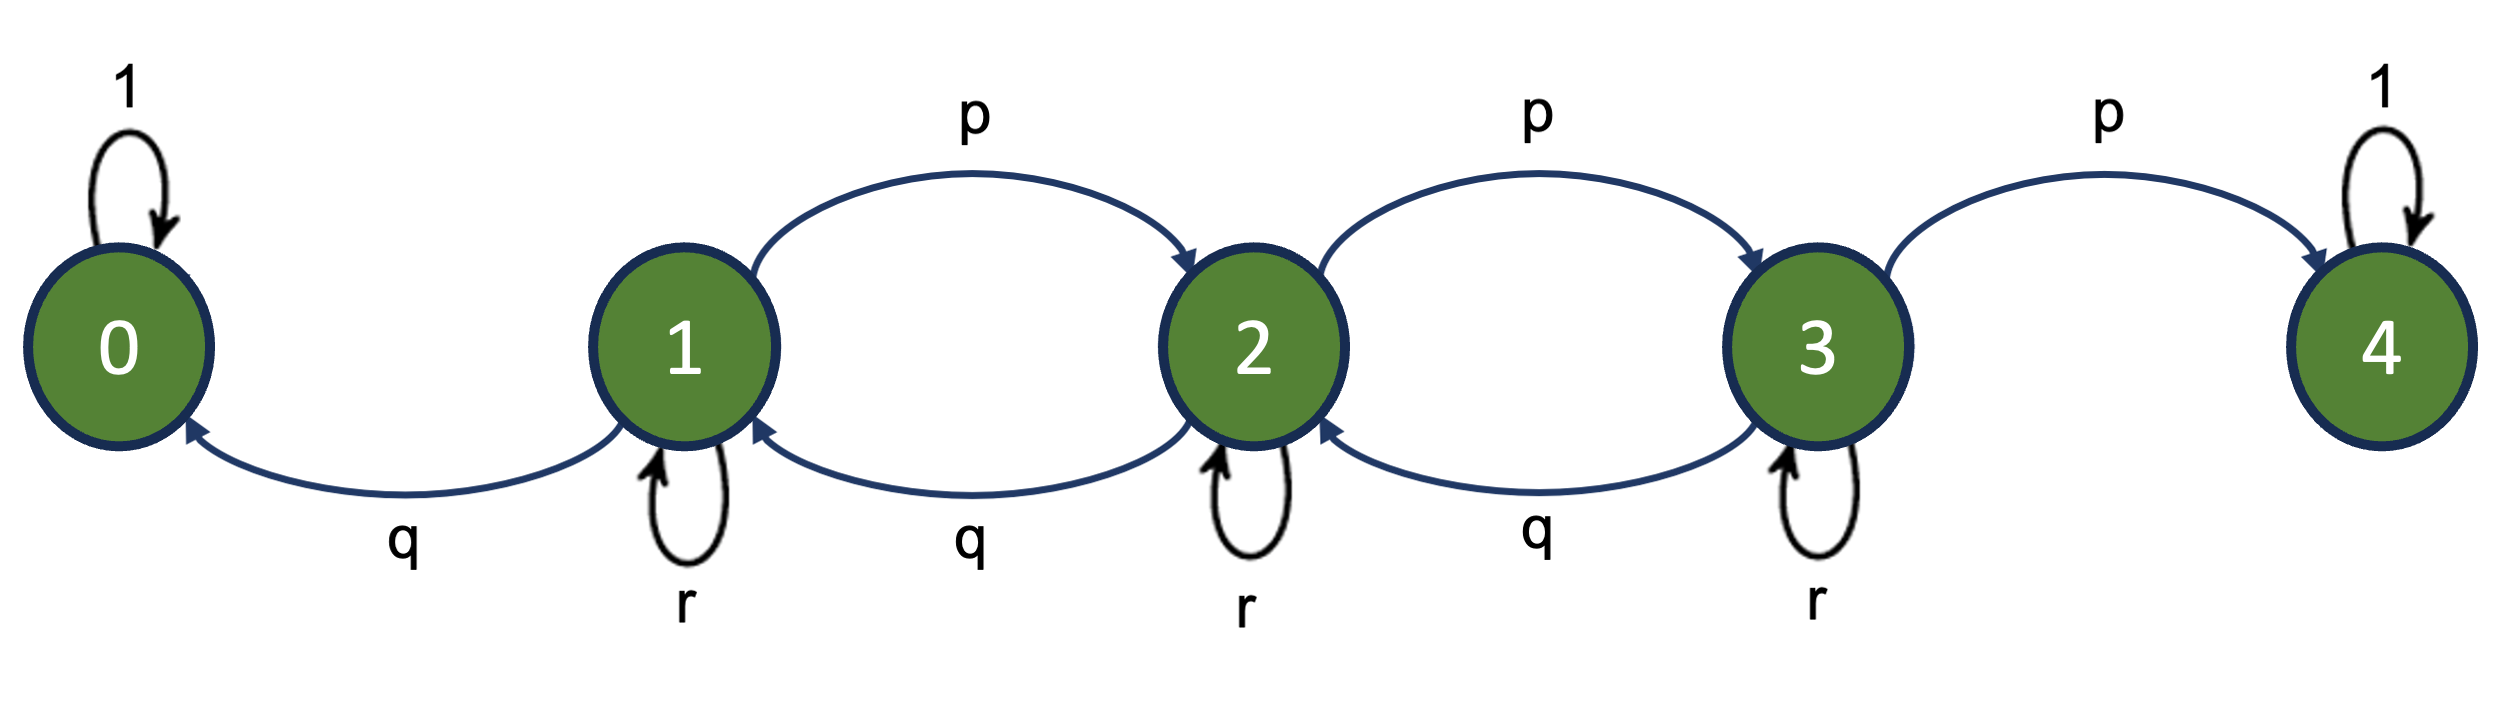
\includegraphics[width=12cm]{diagram.png}
        \caption[Markov chain state diagram even-money payoff case.] {\textit{State diagram for $N$ = 4 even-money payoff case}. The diagram includes 5 nodes to indicate the possible states $S = \{0,1,2,3,4\}$ the Markov chain $S_{n}$ can take. States $0$ and $4$ are absorbing states.} \label{fig:diagram}
\end{figure}
Once the Markov chain to model the gambler's capital has been defined, it is important state the 3 fundamental questions related to the gambler's ruin problem that would help to construct further knowledge. Firstly, the inquiry into whether the gambler can continue betting indefinitely after the game ends sheds light on the finite nature of the problem and the boundaries it imposes. Secondly, determining the probability of the gambler getting ruined provides insights into the inherent risks involved in gambling, with implications for risk management and decision-making. Lastly, investigating the expected duration of the game offers insights into the average number of steps or rounds required for the game to finish.

\subsubsection{Finite nature of the game}\label{finite_nature}
To answer whether the game will end in a finite number of rounds or if the gambler would continue to bet against the casino an infinite number of times we need to define the concept of accessibility, communication, and some other Markov chain properties included in \cite{kulkarni, feller}.

\begin{Definition} A state $j$ is said to be accessible from state $i$ if there is a way to go from state $i$ to state $j$. It is denoted by $i \rightarrow j$.
\end{Definition}

Accessibility is easy to detect using a state diagram (see Figure \ref{fig:diagram}). $i \rightarrow j$ is equivalent to find a   path from node $i$ to node $j$. 

\begin{Definition} States $i$ and $j$ are said to communicate if $i \rightarrow j$ and $j \rightarrow i$ and it is denoted by $i \leftrightarrow j$.
\end{Definition}

Communication is an equivalence relation since it fulfils the following properties:
\begin{enumerate}
    \item Reflection. $i \leftrightarrow i$ for all state $i \in S$
    \item Symmetry. If $i \leftrightarrow j$ then $j \leftrightarrow i$
    \item Transitivity. If $i \leftrightarrow j$ and $j \leftrightarrow k$ then $i \leftrightarrow k$
\end{enumerate}

This equivalence relation classifies all the states in $S$ into equivalence classes which are subsets of $S$ which includes all elements that are equivalent to each other. In that sense, two distinct communicating classes are disjoint.

\begin{Definition}
A communicating class $C \subseteq S$ is said to be closed if $i\in S$ and $j\notin S$ implies that $j$ is not accessible from $i$.
\end{Definition}

The concept of closed communicating classes is essential in understanding the game's dynamics. In this case, there are two closed communicating classes: $\{0\}$, $\{N\}$, representing the ruin and total capital states, respectively. Once the gambler reaches either of these states, they cannot transition to any other state and in our context, the game is over. Furthermore, the fact that the communicating class $T=\{1,...,N-1\}$ is not closed indicates that there is a possibility of leaving the class and since the other classes in the system are closed, once the chain leaves the class $T$ there is no way to go back to it.  Hence, eventually, the chain will reach one of the closed communicating classes, ensuring the game's termination and regardless the value of $p,q$ and $r$ provided $r\neq 1$.

The game's finite nature ensures that in the long term, the Gambler's ruin problem yields only two possible outcomes for the gambler: winning all the capital or getting ruined. 

\subsubsection{Probability of ruin}
The next important question is to determine the probability of getting ruined. This probability, known as the Gambler's ruin probability, can be calculated by formulating the problem as a second-order homogeneous linear difference equation with two boundary conditions, as explained in \cite{feller}. In this regard, the first passage probability comes into play as a useful tool:

\begin{Definition}Let $T_{A} = min\{n\geq 1 : S_{n}\in A\}$ be the first passage time of the Markov chain $S_{n}$ to a set $A \subset S$. If the chain never reaches the set A then $T_{A} = \infty$.  
\end{Definition}

Let $A = {0}$ and $B = {N}$. We are interested in finding the probability of the gambler’s ruin given the initial capital is $z$:
\begin{eqnarray}
    q_{z} = P(T_{A}<T_{B} \text{\textbar} S_{0}= z).
\end{eqnarray}

\begin{eqnarray}
    q_{z} &=& P(T_{A}<T_{B} \text{\textbar} S_{0}= z)\notag\\
&=& \sum_{j\in S}P(T_{A}<T_{B} \text{\textbar} S_{1} = j, S_{0}= z) P(S_{1}= j \text{\textbar} S_{0}= z)\notag\\
&=& \sum_{j\in S}P(T_{A}<T_{B} \text{\textbar} S_{1} = j) P(S_{1}= j \text{\textbar} S_{0}= z)\notag\\
&=& \sum_{j\in S}P(T_{A}<T_{B} \text{\textbar} S_{0} = j) P(S_{1}= j \text{\textbar} S_{0}= z)\notag\\
&=& \sum_{j\in S}q_{j}P(S_{1}= j \text{\textbar} S_{0}= z).\label{exp_1}  
\end{eqnarray}

Since the gambler's capital can move by at most 1 unit each round, (\ref{exp_1}) can be rewritten as follows:
\begin{eqnarray}
q_{z} &=&  p  q_{z+1}+ q q_{z-1} +  rq_{z} \notag\\
&=&  \frac{p  q_{z+1}+ q q_{z-1}}{1-r} \notag\\
&=& p^{*}  q_{z+1}+ q^{*} q_{z-1}, \label{exp_2} 
\end{eqnarray}

where $p^{*} = p/(1-r)$ and $q^{*} = q/(1-r)$. Expression (\ref{exp_2})  is valid for $1\leq z \leq N-1 $ and has the following boundary conditions 
\begin{eqnarray}
q_{0} = 1, & q_{N} = 0.
\label{exp_3} 
\end{eqnarray}

$q_{0} = 1$ because the probability of ruin, given the gambler starts with no capital, is one. In other words, the probability of getting ruined, given that he is already ruined, is one. On the other hand, $q_{N} = 0$ because the probability of getting ruined, given the gambler has already won all opponent's capital, is zero.

Now, using that $p^{*} + q^{*} = 1$
\begin{eqnarray}
(p^{*} + q^{*})q_{z} &=&  p^{*}  q_{z+1}+ q^{*} q_{z-1}. \notag 
\end{eqnarray}
equivalently:

\begin{eqnarray}
q_{z-1}- q_{z} &=&  \frac{p^{*}}{q^{*}}(q_{z}- q_{z+1}) = \frac{p}{q}(q_{z}- q_{z+1}). \notag
\end{eqnarray}

for $z = N-1$:

$$q_{N-2} - q_{N-1} = \frac{p}{q}(q_{N-1} - q_{N}) = \frac{p}{q}q_{N-1}.$$

for $z = N-2$ recursively: 

$$q_{N-3} - q_{N-2} = \frac{p}{q}(q_{N-2} - q_{N-1}) = \frac{p}{q}\left(\frac{p}{q}q_{N-1} \right)= \left(\frac{p}{q}\right) ^{2}q_{N-1}.$$

In general:
\begin{eqnarray}
q_{N-(i+1)}- q_{N-i} &=& \left(\frac{p}{q}\right) ^{i} q_{N-1}. \notag
\end{eqnarray}

using the telescopic sum
\begin{eqnarray}
q_{N-z}- q_{N-1} &=&(q_{N-z}- q_{N-(z-1)}) + (q_{N-(z-1)}- q_{N-(z-2)}) + ... + (q_{N-2}- q_{N-1})\notag\\
&=& \left(\frac{p}{q}\right) ^{z-1} q_{N-1} + \left(\frac{p}{q}\right) ^{z-2} q_{N-1} +...+\frac{p}{q}q_{N-1}\notag\\
&=& q_{N-1} \sum_{i =1}^{z-1}\left(\frac{p}{q}\right) ^{i}. \notag
\end{eqnarray}

finally we have:
\begin{eqnarray}
q_{N-z}&=& q_{N-1} + q_{N-1} \sum_{i =1}^{z-1}\left(\frac{p}{q}\right) ^{i}\notag\\
&=& q_{N-1} \sum_{i =0}^{z-1}\left(\frac{p}{q}\right) ^{i} \notag\\
&=& \left\{
\begin{array}{ll}
q_{N-1}\frac{1-(p/q)^{z}}{1-(p/q)} & \text{ if } p\neq q,\\
q_{N-1}(z)& \text{ if } p= q. \label{exp_4}
\end{array}
\right.
\end{eqnarray}

However, we still need to find the value of $q_{N-1}$. If we substitute $z= N$ in \ref{exp_4}:

\begin{eqnarray}
1 = q_{0}&=& \left\{
\begin{array}{ll}
q_{N-1}\frac{1-(p/q)^{N}}{1-(p/q)} & \text{ if } p\neq q,\\
q_{N-1} N& \text{ if } p= q. \notag
\end{array}
\right.
\end{eqnarray}

from which we conclude that
\begin{eqnarray}
q_{N-1}&=& \left\{
\begin{array}{ll}
\frac{1-(p/q)}{1-(p/q)^{N}} & \text{ if } p\neq q,\\
\frac{1}{N}& \text{ if } p= q. \notag
\end{array}
\right.
\end{eqnarray}

Replacing $q_{N-1}$ in \ref{exp_4}, the probability of ruin given an initial capital $i$ is

\begin{eqnarray}
q_{i}&=& \left\{
\begin{array}{ll}
\frac{(q/p)^{N} -(q/p)^{i} }{(q/p)^{N} -1} & \text{ if } p\neq q,\\
1 -\frac{i}{N}& \text{ if } p= q. \label{ruin_proba}
\end{array}
\right.
\end{eqnarray}

The probability of ties, denoted as $r$, does not appear in the probability of ruin expression. This is because, in the context of the gambler's risk of going bankrupt, the crucial factors are the winning and losing probabilities. More precisely, what matters is the ratio between these two parameters, rather than the probability of ties.

\begin{figure}[h!]
  \centering
    \subfigure{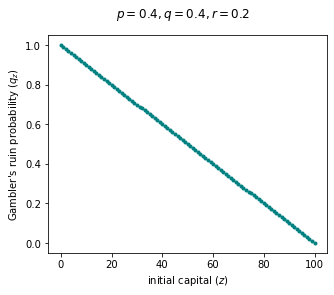
\includegraphics[width=5.2cm]{ruin_p_1.png}}
    \subfigure{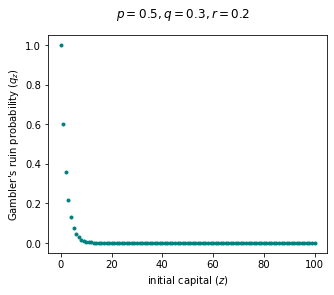
\includegraphics[width=5.2cm]{ruin_p_2.png}}
    \subfigure{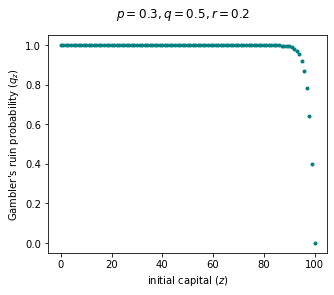
\includegraphics[width=5.2cm]{ruin_p_3.png}}
  \caption[Ruin probability simulation]{\textit{Ruin probability simulation}. The three graphs depict the ruin probability in different gambling scenarios, each characterized by distinct parameters $p,q,r$ but with $N = 100$.}  
  \label{fig:ruin_proba}
\end{figure}

When $p\neq q$ the ruin probability as a function of the initial capital shows a nonlinear pattern. However, the specific shape of the graph depends on whether $p > q$ or vice versa. If $p > q$, the graph initially shows a sharp decrease in the ruin probability, followed by a slower decline as the initial capital increases. On the other hand, if $p < q$, the graph shows a steep descent in the ruin probability as the initial capital increases. In the scenario where $p = q$ the probability of ruin has a linear relationship with respect to the initial capital, represented by a negative slope of $1/N$. 

Regardless of the specific settings of the gambling game, one consistent finding remains: if the gambler starts with a small initial capital compared to the casino's capital, the probability of getting ruined is close to 1. This observation highlights the disadvantage faced by the gambler when he has limited resources compared to the house.

In the limit case where $N \rightarrow \infty$, representing a casino with infinite capital, expression (\ref{ruin_proba}) is simplified to:
\begin{eqnarray}\label{limit_case}
q_{i}&=& \left\{
\begin{array}{ll}
(q/p)^{i} & \text{ if } p > q,\\
1 & \text{ if } p\leq q.
\end{array}
\right.
\end{eqnarray}

In this limiting scenario, the ruin probability follows different patterns depending on the relationship between $p$ and $q$. If $p > q$, the probability of ruin decreases exponentially as the gambler's capital increases. Conversely, if $p \leq q$, the ruin probability remains constant and equal to 1, indicating an inevitable bankruptcy for the gambler in the long run. However, in practice, gamblers usually set finite profit targets rather than aiming for infinite capital, as this provides a more realistic and achievable goal. Let $G$ be the profit target. In this finite scenario, the probability of going bankrupt before reaching $G+z$ is given by a modified version of the ruin probability formula:

\begin{eqnarray}
q_{z, G}&=& \left\{
\begin{array}{ll}
\frac{(q/p)^{G+z} -(q/p)^{z} }{(q/p)^{G+z} -1} & \text{ if } p\neq q,\\
1 -\frac{z}{z+G}& \text{ if } p= q. \label{gral_ruin_proba}
\end{array}
\right.
\end{eqnarray}

Using the finite nature of the game explained in subsection \ref{finite_nature}, the probability of reaching the goal $G$, denoted as $P_{z,G}$, can be calculated as $1-q_{z,G}$:

\begin{eqnarray}
p_{z, G}&=& \left\{
\begin{array}{ll}
\frac{(q/p)^{z} -1}{(q/p)^{G+z} -1} & \text{ if } p\neq q,\\
\frac{z}{z+G}& \text{ if } p= q. \label{reach_proba}
\end{array}
\right.
\end{eqnarray}

Let's suppose the gambler aims to double his initial capital $z$. The probability of doubling his fortune before bankrupt is:
\begin{eqnarray*}
P_{z, z}&=& \frac{1}{(q/p)^{z} +1}. 
\end{eqnarray*}

Such a probability depends on the size of $z$. For example, let's suppose a gambler that is betting on the red numbers in the European roulette\footnote{In this case, $p = 18/37, q = 1-p = 19/37, r = 0$.}, the probability of doubling the initial capital for different values of $z$ is presented in Table \ref{prob_example}. As the initial capital becomes larger, the probability drops significantly to nearly zero.

\begin{table}[h!]
\centering
\caption{Probability of doubling the initial capital betting on red numbers} \label{prob_example}
\begin{tabular}{|c|c|c|c|c|c|}
\hline
$z$ & 1 & 10 &  100 &  1,000 & 10,000\\
\hline
\hline
$p_{z,z}$&0.486&0.368&0.004&0.330 x $10^{-23}$& 0.155x $10^{-234}$\\
\hline
\end{tabular}
\end{table}


\subsubsection{Expected duration of the game}
The expected number of rounds or expected duration of the game, provides an estimate of how long the gambler can expect to play before reaching their profit goal or going bankrupt.

Even if the probability of reaching the goal is attractive for the gambler, he needs to know the expected duration of the game to make informed decisions about their betting strategy. If the expected duration is too long, the gambler may not be willing to invest a significant amount of time and money into the game. On the other hand, if the expected duration is short, the gambler may be more inclined to take risks and play more aggressively to reach their profit goal quickly.

\begin{figure}[h!]
  \centering
    \subfigure{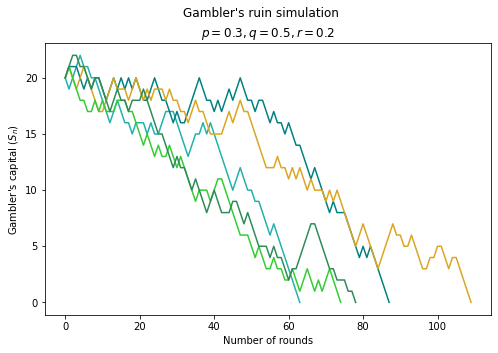
\includegraphics[width=7.5cm]{1simulation.png}}
    \subfigure{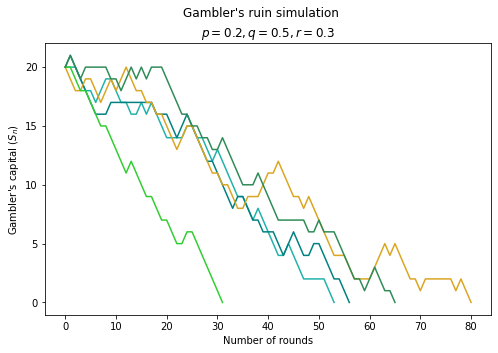
\includegraphics[width=7.5cm]{2simulation.png}}
  \caption[Gambler's ruin simulation]{\textit{Gambler's ruin simulation}. 5 simulated paths of $S_{n}$ are represented in each graph starting with $z = 20$. On the left- hand side the parameters were $p = 0.3, q= 0.5, r=0.2$ and the number of rounds until ruins are between 60 and 120 while on the right-hand side the parameters were $p = 0.2, q= 0.5, r=0.3$ and the number of rounds until ruins are between 30 and 80.}  
  \label{fig:random_walk}
\end{figure}

Using the first passage time definition we can define the following expected value:

\begin{Definition}
    Let $A\subset S$. If $P(T_{A} <\infty  \text{\textbar} S_{0}= i) = 1$ for all $i \in S$, then the mean time to reach $A$ when starting from state $z$ is given by $E_{z} = E(T_{A} \text{\textbar} S_{0}= z)$. 
\end{Definition}

Let $A = \{0,N\}$ be the set of absorbing states, the expected duration of the game is:
\begin{eqnarray}
E_{z} &= &E(T_{A} \text{\textbar} S_{0}= z) \notag\\[12pt]
&= & \sum_{j\in S}E(T_{A} \text{\textbar} S_{1} = j, S_{0}= z) P(S_{1}= j \text{\textbar} S_{0}= z)\notag\\
&=& \sum_{j\in S}E(T_{A} \text{\textbar} S_{1} = j) P(S_{1}= j \text{\textbar} S_{0}= z)\notag\\
&=& \sum_{j\in S}E(T_{A} + 1\text{\textbar} S_{0} = j) P(S_{1}= j \text{\textbar} S_{0}= z)\notag\\
&=& \sum_{j\in S}(E_{j} + 1 )P(S_{1}= j \text{\textbar} S_{0}= z)\notag\\
&=& \sum_{j\in S}E_{j}P(S_{1}= j \text{\textbar} S_{0}= z) + \sum_{j\in S}P(S_{1}= j \text{\textbar} S_{0}= z)\notag\\
&=& \sum_{j\in S}E_{j}P(S_{1}= j \text{\textbar} S_{0}= z) + 1.\label{exp_5} 
\end{eqnarray}

Now, again using the fact that the gambler's capital can change by at most 1 unit per round and $r \neq 1$, (\ref{exp_5}) can be rewritten as follows:
\begin{eqnarray}
E_{z} &=&  p  E_{z+1}+ q E_{z-1} +  rE_{z} + 1\notag\\[12pt]
&=&  \frac{p  E_{z+1}+ q E_{z-1} + 1}{1-r} \notag\\
&=& p^{*}  E_{z+1}+ q^{*} E_{z-1} +  \frac{1}{1-r}. \label{exp_6} 
\end{eqnarray}

Last expression has two boundaries conditions:
\begin{eqnarray}
E_{0} = 0, & E_{N} = 0.
\label{exp_7} 
\end{eqnarray}

Boundary conditions imply that when starting from state $0$ (no capital) or $N$ (having all the capital), the expected duration to reach the absorbing states (0 or N) is zero. This makes intuitive sense since either the gambler has already reached the ruin state or has already achieved their goal, no further round of the game is needed.

Now, using that $p^{*} + q^{*} = 1$
\begin{eqnarray}
(p^{*} + q^{*})E_{z} &=&  p^{*}  E_{z+1}+ q^{*} E_{z-1} + \frac{1}{1-r}.\notag 
\end{eqnarray}
equivalently:

\begin{eqnarray}
E_{z+1}- E_{z} &=&  \frac{q^{*}}{p^{*}}(E_{z}- E_{z-1})-\frac{1-r}{p (1-r)}  = \frac{q}{p}(E_{z}- E_{z-1}) - \frac{1}{p}.  \notag
\end{eqnarray}

for $z = 1$:

$$E_{2}- E_{1} =  \frac{q}{p}(E_{1}- E_{0}) - \frac{1}{p} =  \frac{q}{p}E_{1} - \frac{1}{p} = \frac{1}{p} (qE_{1} -1).$$

for $z = 2$:

$$E_{3}- E_{2} =  \frac{q}{p}(E_{2}- E_{1}) - \frac{1}{p} =  \frac{q}{p}\left(\frac{1}{p} (qE_{1} -1)\right)- \frac{1}{p} = \left(\frac{q}{p}\right)^2E_{1} -\frac{q}{p}\frac{1}{p} - \frac{1}{p}.$$

In general:
\begin{eqnarray}
    E_{z+1}- E_{z} = \left(\frac{q}{p}\right)^zE_{1} - \left(\frac{q}{p}\right)^{z-1}\frac{1}{p}-...-\frac{q}{p}\frac{1}{p} - \frac{1}{p} =\left(\frac{q}{p}\right)^zE_{1} - \frac{1}{p}\sum_{i=0}^{z-1}\left(\frac{q}{p}\right)^{i}.
\end{eqnarray}

And using the telescopic sum: 
\begin{eqnarray}
    E_{z+1}- E_{1} &=& (E_{z+1}- E_{z}) + (E_{z}- E_{z-1})+...+ (E_{2}-E_{1})\notag\\[15pt]
    &=& \sum_{i=1}^{z}\left(\frac{q}{p}\right)^{i}E_{1} - \frac{1}{p}\sum_{j=0}^{z-1}\sum_{i=0}^{j}\left(\frac{q}{p}\right)^{i}.\notag
\end{eqnarray}

Then, 
\begin{eqnarray}\label{e_z_1}
    E_{z+1} &=& E_{1} + \sum_{i=1}^{z}\left(\frac{q}{p}\right)^{i}E_{1} - \frac{1}{p}\sum_{j=0}^{z-1}\sum_{i=0}^{j}\left(\frac{q}{p}\right)^{i}\notag\\
    &=& \sum_{i=0}^{z}\left(\frac{q}{p}\right)^{i}E_{1} - \frac{1}{p}\sum_{j=0}^{z-1}\sum_{i=0}^{j}\left(\frac{q}{p}\right)^{i}.
\end{eqnarray}

Evaluating $z = N-1$ in (\ref{e_z_1}) we have:

\begin{eqnarray}\label{e_1}
E_{1}&=& \left\{
\begin{array}{ll}
\frac{N}{p \left(1 - \left(\frac{q}{p}\right)^{N}\right)} - \frac{1}{p-q}& \text{ if } p\neq q,\\[20pt]
\frac{N-1}{1-r}& \text{ if } p= q. 
\end{array}
\right.
\end{eqnarray}

And finally, the expected duration of the game starting with capital $z$ is given by: 
\begin{eqnarray}\label{e_z}
E_{z}&=& \left\{
\begin{array}{ll}
\frac{z}{q-p} - \frac{N}{q-p}\frac{1 - \left(\frac{q}{p}\right)^{z}}{1 - \left(\frac{q}{p}\right)^{N}}& \text{ if } p\neq q,\\[12pt]
\frac{z(N-z)}{1-r}& \text{ if } p= q. 
\end{array}
\right.
\end{eqnarray}

The value of $r$ that were not taken into account in the ruin probability does indeed affect the expected numbers of rounds. As $r$ increases the expected number of rounds increases exponentially (see Figure \ref{fig:variation_r}). In other words, a higher value of $r$ means that there's a greater chance that bets will result in a draw, leading to more rounds being played on average before a final outcome is reached. This behavior is intuitive, as the presence of ties introduces uncertainty and delays in determining the ultimate result of the game.

\begin{figure}[h!]
  \centering
    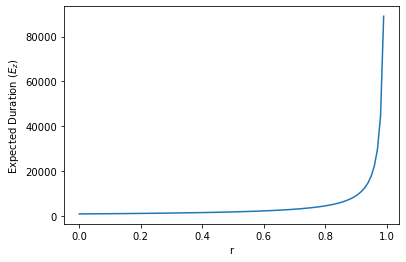
\includegraphics[width=9cm]{r_variation.png}
  \caption[Expected duration of the game as a function of $r$]{\textit{Expected duration of the game as a function of $r$}. As $r$ increases the expected number of rounds increases exponentially. In this example $z = 10$, $N = 100$, $p = q = (1-r)/2$.}  
  \label{fig:variation_r}
\end{figure}

The concave nature of (\ref{e_z}) indicates the duration of the game increases as the gambler's capital $z$ increases, reaches a maximum point at $z^{*}$, and then starts decreasing as $z$ continues to increase beyond $z^{*}$. The critical point $z^{*}$ is where the duration of the game is maximized. When starting the game with a lower capital, the gambler is more likely to lose quickly. Conversely,  when starting the game with a capital higher than $z^{*}$, the gambler is more likely to reach the goal quickly.
 \begin{eqnarray}
z^{*}&=& \left\{
\begin{array}{ll}
\frac{\log\left(\frac{N(q-p)}{q-p - (q/p)^N}\right)}{\log\left(\frac{q}{p}\right)}& \text{ if } p\neq q,\\[15pt]
\frac{N}{2}& \text{ if } p= q. 
\end{array}
\right.
\end{eqnarray}

Figure (\ref{fig:duration}) depicts the expected duration of the gambling game under various scenarios. Different combinations of $p$, $q$, and $r$ lead to distinct shapes in the expected duration curves.

\begin{figure}[h!]
  \centering
    \subfigure{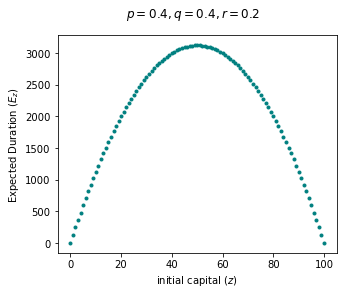
\includegraphics[width=5.2cm]{duration_1.png}}
    \subfigure{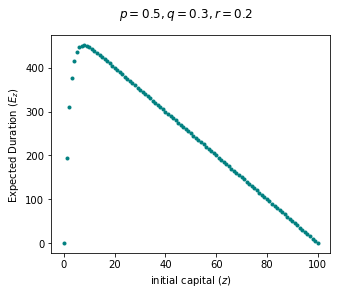
\includegraphics[width=5.2cm]{duration_2.png}}
    \subfigure{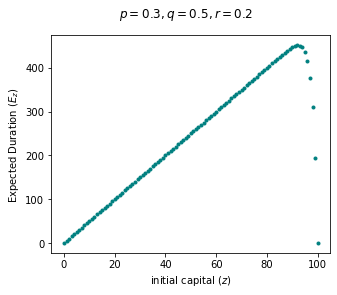
\includegraphics[width=5.2cm]{duration_3.png}}
  \caption[Expected duration of the game simulation]{\textit{Expected duration of the game simulation}. The three graphs depict the expected duration of the game in different gambling scenarios, each characterized by distinct parameters $p,q,r$ but with $N = 100$.}  
  \label{fig:duration}
\end{figure}


In the next subsection, the analysis of the probability of ruin and expected duration will be extended to the case of \textit{m-to-1} payoff bets.

\subsection{\textit{m-to-1} payoff problem}
Let's compute the probability of ruin formula in the case of an \textit{m-to-1} payoff. Let $m$ be a positive integer, and assume that the gambler's betting 1 unit and there are 3 three possible outcome values: a win with a payout of $m$, a loss with a payout of $-1$, or a tie with a payout of $0$.

\begin{equation}
X_{i} = \left\{
\begin{array}{rl}
m & \text{ with probability = } p,\\
-1 & \text{ with probability = } q,\\
0 & \text{ with probability = } r.
\end{array}
\right.
\end{equation}\label{x_i_ext}

This redefinition of the random variables $X_{i}$ does not change the definition of the Markov chain $S_{n}$ that represents the gambler's capital presented in (\ref{capital}). Nevertheless, the introduction of \textit{m-to-1} payoff changes the dynamics of the $S_{n}$. It can either stay in the same state (remain at the current capital), move $m$ positions to the right (win the bet), or move $1$ position to the left (lose the bet) (see example in Figure \ref{fig:diagram_2}). This introduces more complexity to the analysis of the ruin probability.

\begin{figure}[ht]
        \centering
        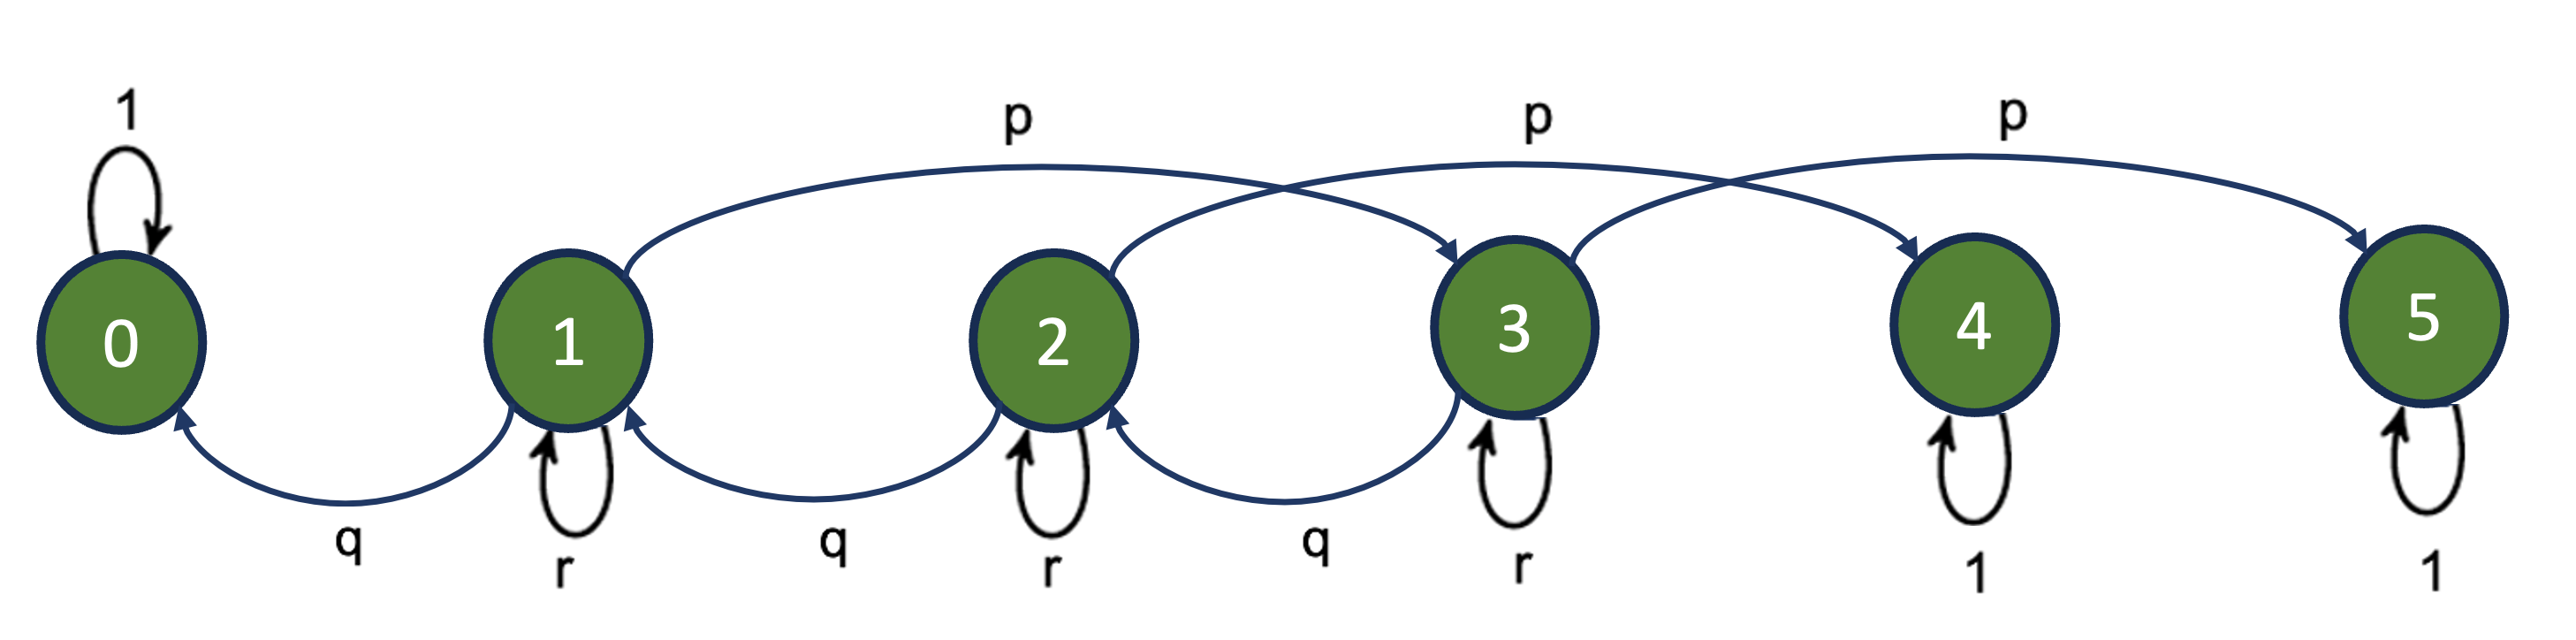
\includegraphics[width=12cm]{diagram_2.png}
        \caption[Markov chain state diagram \textit{m-to-1} payoff case.] {\textit{State diagram for $N$ = 4, and 2 to 1 payoff}. The diagram includes 6 nodes to indicate the possible states $S = \{0,1,2,3,4,5\}$ the Markov chain $S_{n}$ can take. States $0$, $4$ and $5$ are absorbing states.} \label{fig:diagram_2}
\end{figure}

\subsubsection{Finite nature of the game}
Similar to the even-money payoff case, in the \textit{m-to-1} payoff situation, there exists one not closed communicating class $T = \{1,...,N-1\}$ that allows the chain to transition to other communicating classes, which are closed. Nevertheless, in the \textit{m-to-1} payoff setup there are  $m+1$ closed communicating classes: $\{0\}$, $\{N\}$, $\{N+1\}$, ..., $\{N+m-1\}$, each associated with an absorbing state.

Thus, under the \textit{ m-to-1} payoff scenario, as well as in the even-money payoff case, the finite nature of the game is ensure. In that sense, there are only two possible outcomes for the gambler, either winning all the capital or getting ruined. 

\subsubsection{Probability of ruin}

The probability of getting ruined given an initial capital of $z$ is given by the recursive equation:
\begin{eqnarray}
q_{z} &=&  p  q_{z+m}+ q q_{z-1} +  rq_{z} \notag\\
&=&  \frac{p  q_{z+m}+ q q_{z-1}}{1-r} \notag\\
&=& p^{*}  q_{z+m}+ q^{*} q_{z-1}, 
\end{eqnarray}

with boundary conditions: 
\begin{eqnarray}
q_{0} = 1, & q_{N} =q_{N+1}=...= q_{N+m-1}= 0.
\end{eqnarray}

These boundary conditions reflect the fact that if the gambler reaches state $0$ he is already ruined, and if he reach any of the states $N, N+1, ..., N+m-1$, his corresponding ruin probability is zero since he reached at least the goal $N$ and the game is over.

The solution of this second-order homogeneous linear difference equation is presented in \cite{chances}: 
\begin{eqnarray}
q_{z} =  \left\{
\begin{array}{ll}
\frac{q^{z}a(N-z)}{(p+q)^{z}a(N)} & \text{ if } p\neq q,\\[10pt]
\frac{2^{-z}a(N-z)}{a(N)} & \text{ if } p= q, 
\end{array}
\right. 
\end{eqnarray}\label{gral_proba}

where the function $a(k)$ is defined as follows: 
\begin{eqnarray*}
a(k) = \sum_{j=0}^{\lfloor (k-1)/(m+1)\rfloor} (-1)^{j} \binom{k -jm -1}{j} \left(\frac{pq^{m}}{(p+q)^{m+1}}\right)^{j}.
\end{eqnarray*}

A distinction arises from the even-money payoff case due to the presence of the parameter $r$, which is incorporated into the expression for the probability of ruin through the relationship $p+q = 1-r$. This relationship becomes particularly clear when $p = q$. In such case, the expression for the probability of ruin (\ref{gral_proba}) is simplified since the term $(p+q)^z$ simplifies to $(2p)^z$, and the denominator becomes $a(N)$. This probability of ruin computation draws upon the principles of a binomial distribution, which takes into account the distribution of both gains and losses across rounds.

\subsubsection{Expected duration of the game}

In the case of the \textit{m-to-1} payoff, computing the expected value of the number of rounds required to reach the profit goal or to go bankrupt is generally more complex compared to the even-money payoff case.

Obtaining a closed-form or analytical expression for the expected number of rounds is challenging or just not possible in some cases. Instead, one typically relies on numerical methods or simulation-based approaches to estimate the expected number of rounds. By running simulations of the gambling process many times and averaging the number of rounds required in each simulation, one can obtain an approximate value for the expected number of rounds.\\

Table \ref{diff_bets}  presents estimations for the ruin probability and expected game duration under different payoff bets in a gambling scenario where the gambler starts with an initial capital of 50, aiming to reach a goal of 100 while betting 1 unit at a time. Estimations considered 100,000 simulations for each bet type.
\clearpage
\begin{table}[h!] 
\centering
\caption{Estimation for ruin probability and game duration under different payoff bets when doubling an initial capital of $50$ and betting 1 unit at a time.}
\begin{tabular}{|c|l|c|c|} 
\hline
Bet type  & Payoff & Ruin probability& Game duration\\
\hline\hline
Single & 35 to 1 & 0.5707&89\\
Split  &  17 to 1&0.5708&164\\
Street &  11 to 1&0.5810&243\\
Square &  8 to 1&0.5959&326\\
Six Line/Double Street  & 5 to 1&0.6419&506\\
Dozen & 2 to 1&0.7991&1098\\
Red or Black & 1 to 1 &0.9373&1617\\
\hline
\end{tabular} \label{diff_bets}
\end{table}


By observing Table \ref{diff_bets}, it can be noticed that the ruin probability decreases as the payoff ratio increases. Bets with higher payoffs, such as the single and split bets, offer the possibility of significant gains relative to the initial capital. As a result, they also carry a lower probability of ruin because the jump the capital gets in case of a win is significantly higher. This suggests that gamblers are less likely to go bankrupt when opting for riskier bets with larger potential rewards. Conversely, bets with lower payoffs, like the red or black bets, offer more conservative gains but come with a higher probability of ruin because even when the gambler wins more rounds on average, the amount won makes the capital give just a small jump towards the goal.

The relationship between payoff ratios and expected game duration is also logical. Bets with higher payoffs tend to have a shorter expected duration, as exemplified by the single, split, and street bets. These bets offer the chance for significant winnings in a shorter time frame, which can lead to games concluding more quickly. On the other hand, bets with lower payoffs, such as the dozen or red or black bets, have a longer expected duration.

Seeing the two aspects together, the ruin probability and game duration, we need to recall that roulette is a game with a negative expectation. As the game lasts longer, the gambler's capital will decrease on average, which is reflected in a higher probability of ruin.\\

A more detailed analysis can be conducted by creating histograms that depict the distribution of the number of rounds required, differentiating between cases where the gambler achieves the goal and cases where the gambler faces ruin. Figure \ref{fig:hists_1} showcases a two-column array of histograms: the green graphs represent the estimated probability distribution of the number of rounds until reaching the goal, while the red graphs illustrate the estimated probability distribution of the number of rounds before bankruptcy occurs.

Consistently for the different type of bets, the average number of rounds required to reach the goal is lower than the average number of rounds played before experiencing ruin. This observation suggests that successful strategies tend to achieve the goal more swiftly, while unsuccessful strategies prolong the duration of play before leading to bankruptcy.
\begin{figure}[H]
        \centering
        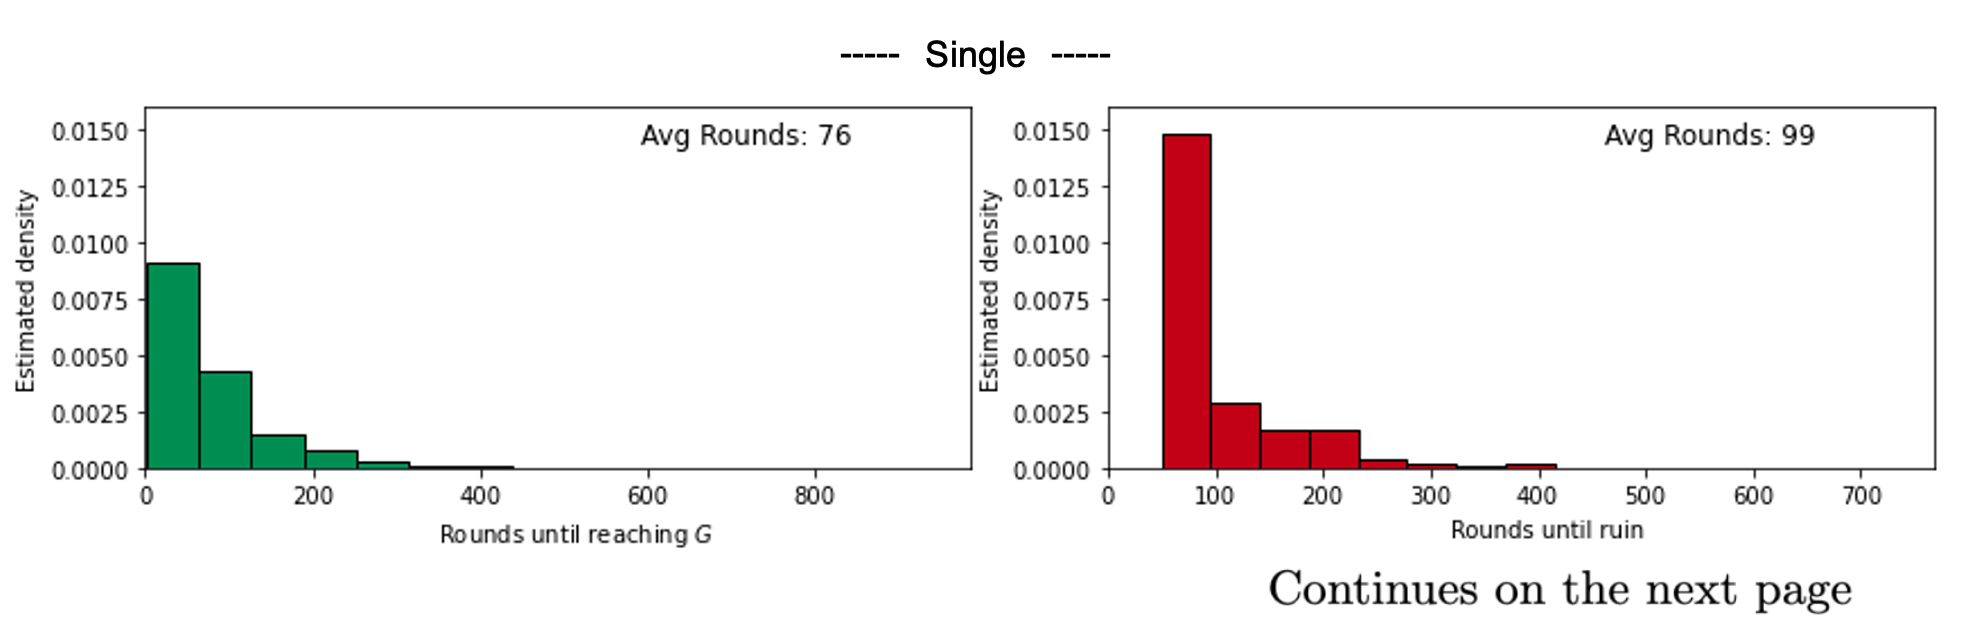
\includegraphics[width=13cm]{cut_1.png}
        \caption* {\textit{Number of rounds distribution comparison: Goal achievement vs. ruin cases - Betting 1 unit at a time}. Across the different types of bets, the average number of rounds needed to achieve the goal (green graphs) is consistently lower than the average number of rounds played before bankruptcy (red graphs).} 
\end{figure}

\begin{figure}[H]
        \centering
        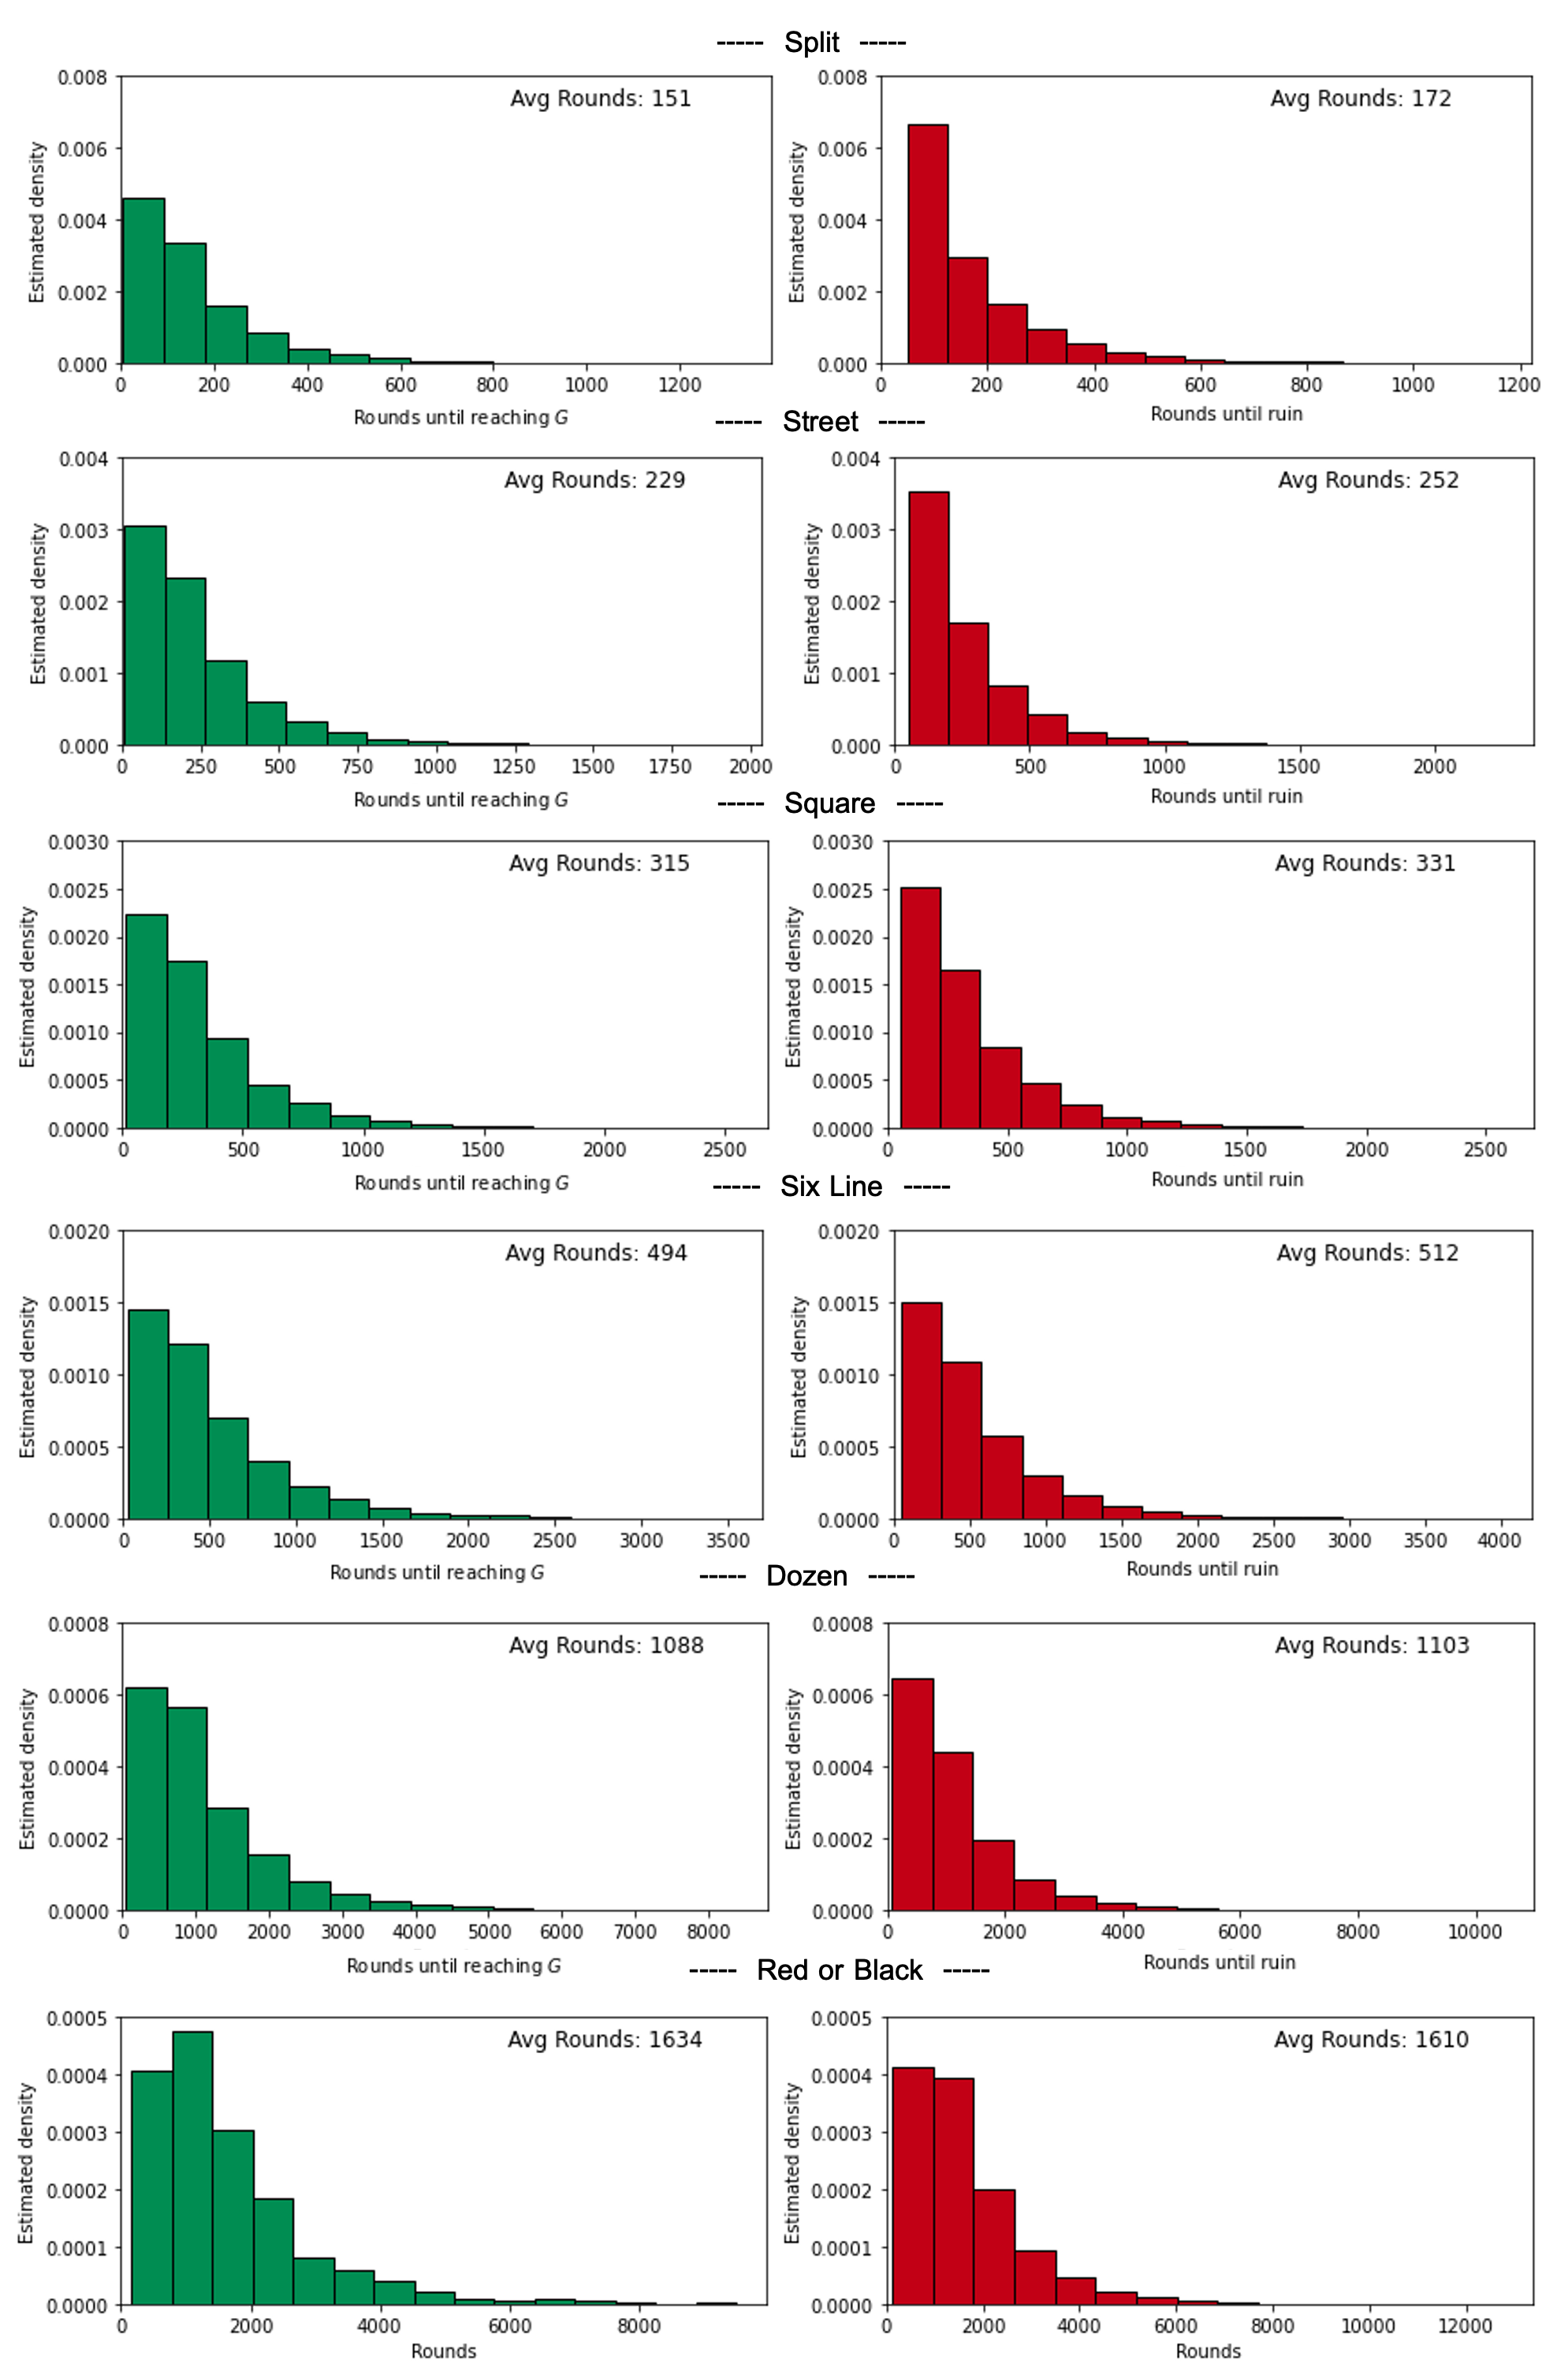
\includegraphics[width=13cm]{cut_2.png}
        \caption[Number of rounds distribution comparison: Goal achievement vs. ruin cases - Betting 1 unit at a time.] {\textit{Number of rounds distribution comparison: Goal achievement vs. ruin cases - Betting 1 unit at a time}. Across the different types of bets, the average number of rounds needed to achieve the goal (green graphs) is consistently lower than the average number of rounds played before bankruptcy (red graphs).} \label{fig:hists_1}
\end{figure}

So far, we have considered scenarios in which the players bet 1 unit at a time, aiming for a reward of $m$. Under this approach, the gambler expects the capital to increase in steps of size $m$, which decreases the average number of rounds as they bet on higher payoff options. However, there is another way to utilize \textit{m-to-1} payoff bets. This alternative strategy offers the advantage of reducing the amount of capital at risk (i.e., the bet amount). For bets with higher payoffs, the amount at risk is proportionally lower ($1/m$).

Nevertheless, it's important to note that due to the constant potential profit of 1 unit, regardless of the chosen bet type, the expected duration of the game is expected to be longer compared to the strategy of betting 1 unit at a time with the objective of reaching a reward of $m$.

One significant implication of adopting this betting approach is the introduction of non-integer capital values in each round. Unlike the previous strategy, where capital was treated as an integer, this strategy allows for rational capital values in each round. This modification results in a more complex state diagram for the Markov chain representing the gambler's progression. Instead of a finite number of states, it involves a countably infinite number of states.

Furthermore, the fractional bet amount of $1/m$ in this strategy reduces the capital at risk in each round, which is proportionally lower for bets with higher payoffs. However, this introduces another nuanced interpretation of ruin. In this context, 'ruin' does not solely mean reaching zero capital but can also signify that the remaining capital falls below a critical level, typically the minimum bet amount allowed in casinos. Even though the capital doesn't fully deplete to zero, it becomes insufficient to sustain further betting at the chosen bet amount. This highlights the need to consider a broader range of possible outcomes and the critical threshold at which the gambler's capital becomes too small to continue their strategy.

Table \ref{diff_bets_1_m} provides estimations for the ruin probability and expected game duration under different payoff bets using the $1/m$ betting strategy. It is assumed that the gambler starts with an initial capital of 50, aiming to reach a goal of 100 while betting 1 unit at a time. The estimations are based on 100,000 simulations for each bet type.

\begin{table}[!ht]
\centering
\caption{Estimation for ruin probability and game duration under different payoff bets when doubling an initial capital of $50$ and betting $1/m$ unit at a time.}
\begin{tabular}{|c|l|c|c|}
\hline
Bet type  & Payoff & Ruin probability& Game duration\\
\hline\hline
Single & 35 to 1 & 0.9417&56,541\\
Split  &  17 to 1&0.9391&27,585\\
Street &  11 to 1&0.9397	&17,823\\
Square &  8 to 1&0.9397	&13,019\\
Six Line/Double Street  & 5 to 1&0.9399	&8,066\\
Dozen & 2 to 1&0.9385	&3,243\\
Red or Black & 1 to 1 &0.9373&1,617\\
\hline
\end{tabular}\label{diff_bets_1_m}
\end{table}

A notable observation is that the ruin probability remains relatively consistent across different bet types when employing the $1/m$ betting strategy. This indicates that, regardless of the type of bet, the probability of the gambler facing ruin is comparable. This suggests that the $1/m$ betting strategy does not significantly alter the risk of ruin based on the chosen bet type.

On the other hand, the expected game duration varies significantly across different bet types. Bets with higher payoffs, such as the single bet, result in considerably longer game durations. This is likely due to the fact that the potential profit remains fixed at 1 unit regardless of the bet type, leading to more rounds needed to reach the goal. Conversely, bets with lower payoffs, like the red or black bet, yield shorter game durations, as the potential profit is consistently smaller, allowing the gambler to approach the goal more rapidly.

Figure \ref{fig:hists_2} shows the histograms of the number of rounds required, differentiating between cases where the gambler achieves the goal and cases where the gambler faces ruin. The histograms in green depict the estimated probability distribution of the number of rounds needed to achieve the desired profit goal, while the red histograms portray the estimated probability distribution of the number of rounds played before facing ruin.

Upon analyzing these histograms, a consistent pattern emerges: the average number of rounds necessary to attain the profit goal is generally lower than the average number of rounds played before encountering bankruptcy. 

\clearpage

\begin{figure}[H]
        \centering
        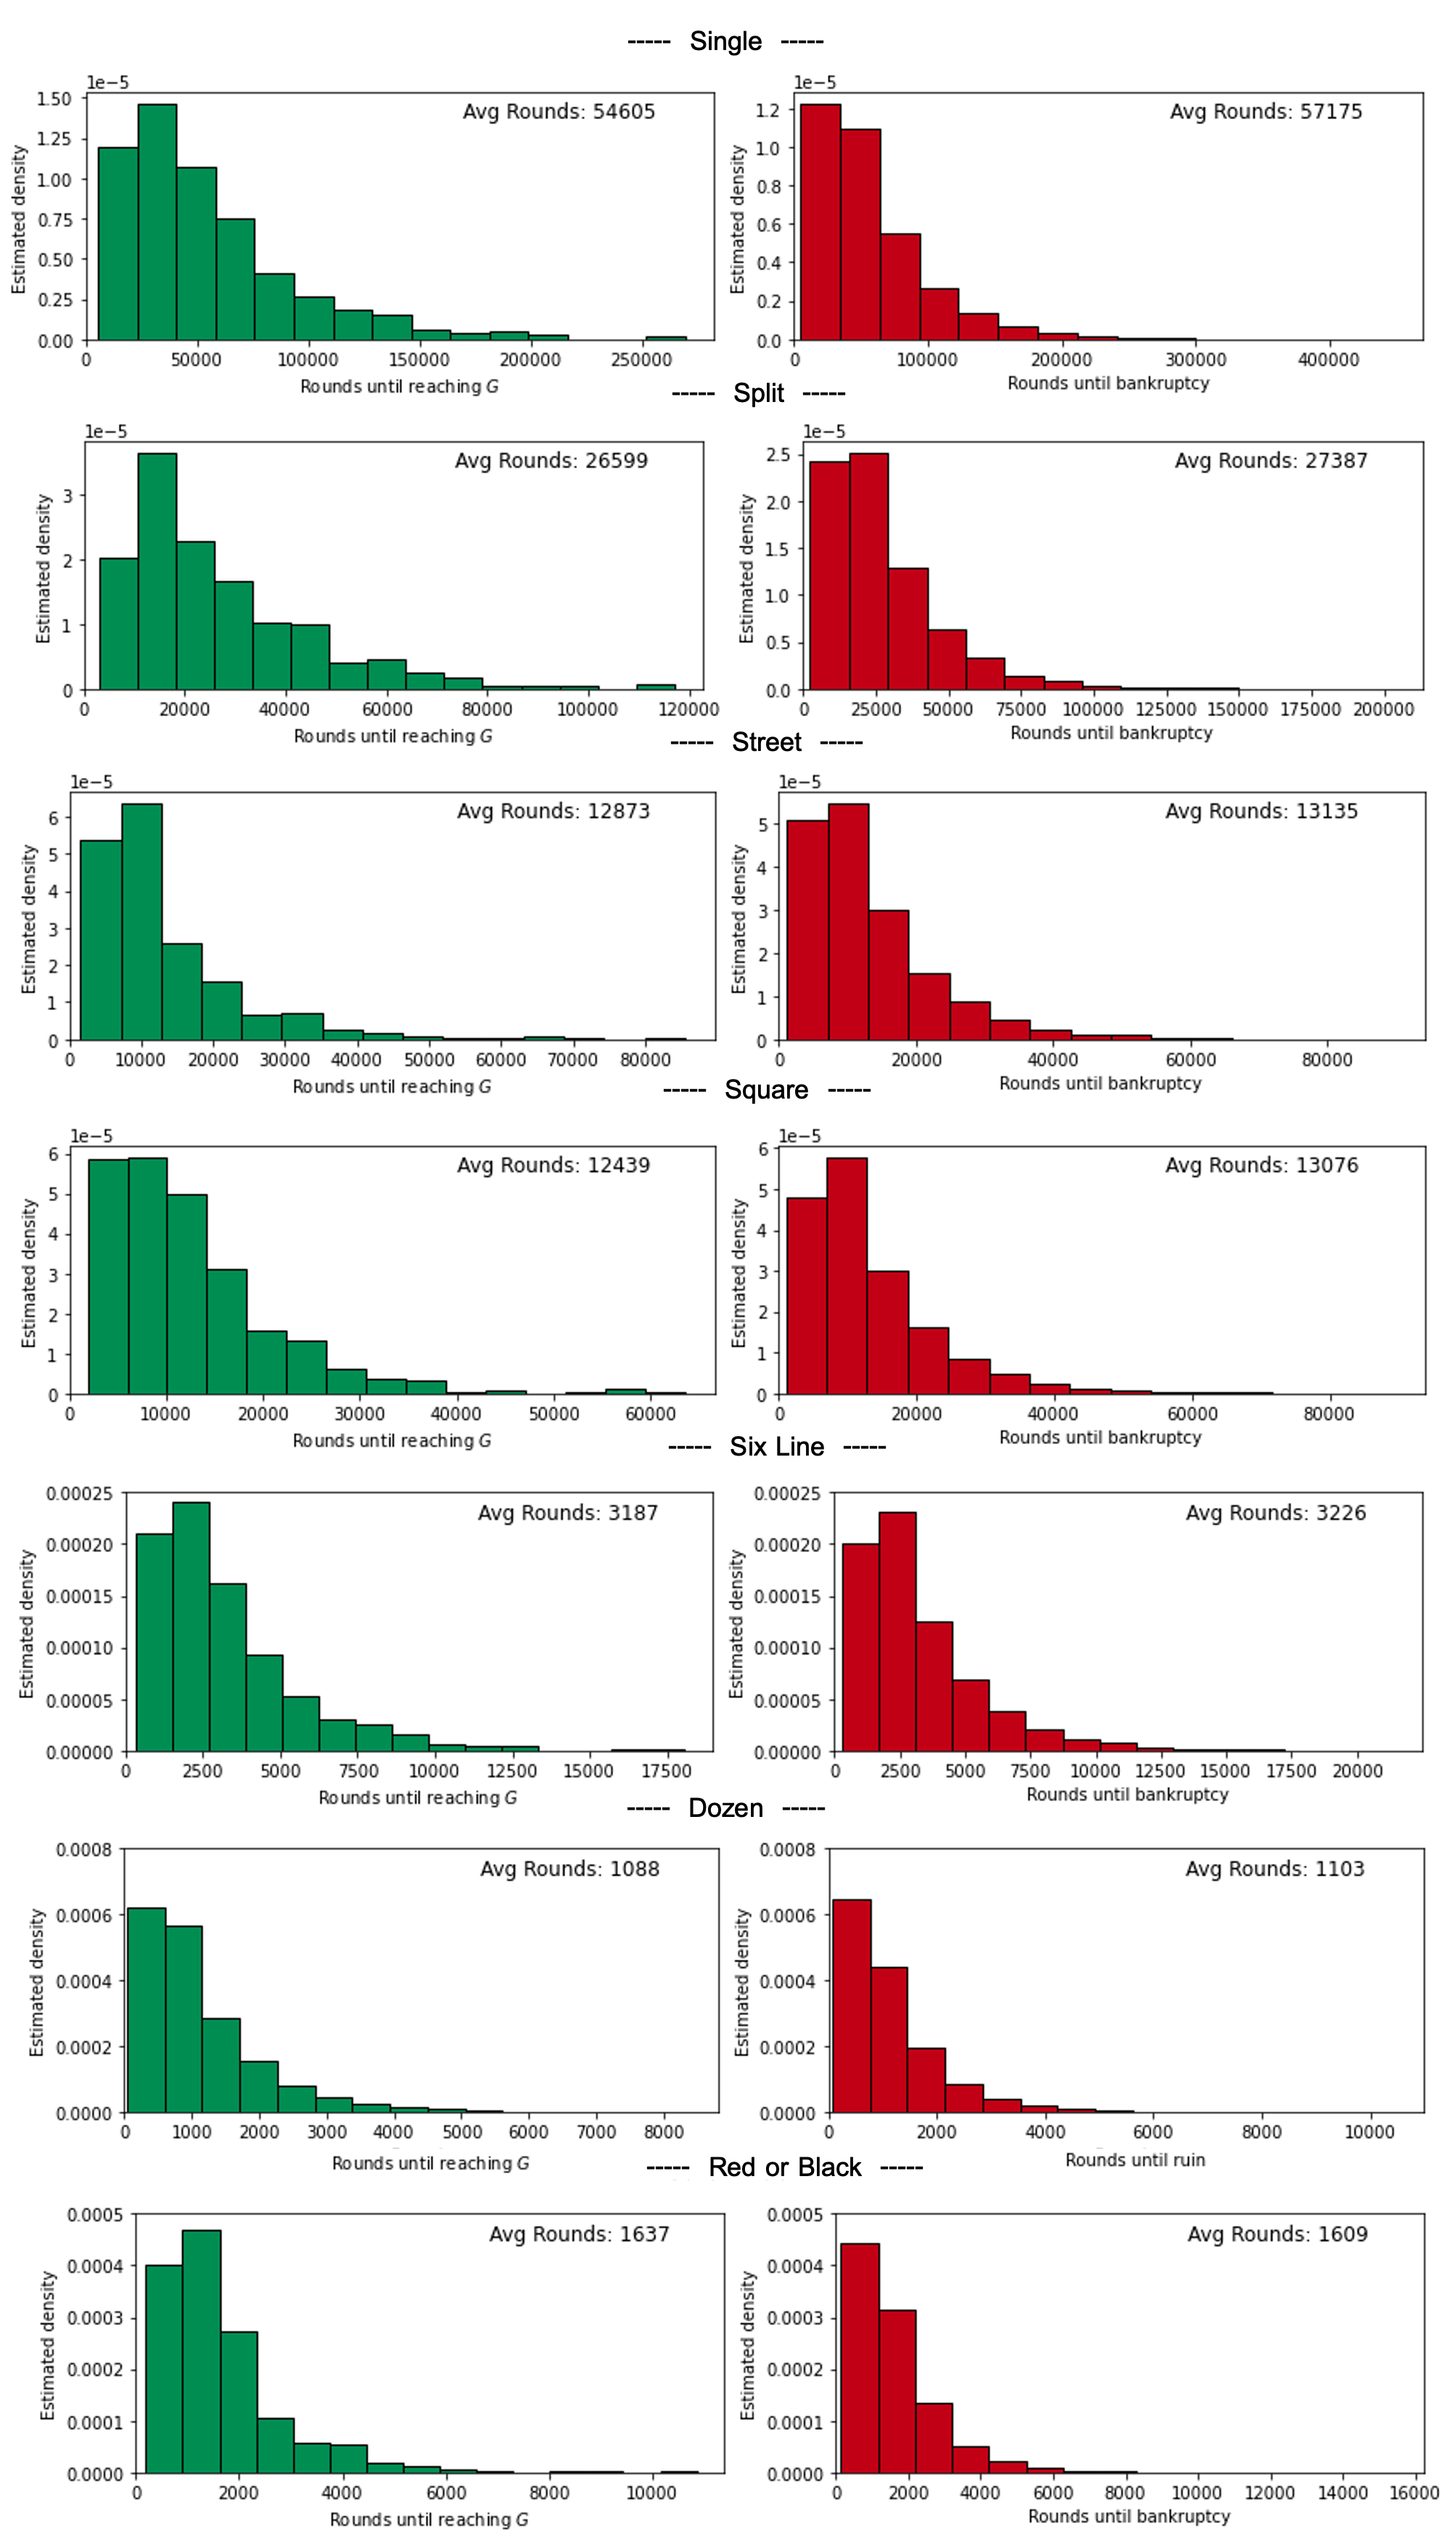
\includegraphics[width=13cm]{hists_2.png}
        \caption[Number of rounds distribution comparison: Goal achievement vs. ruin cases - Betting $1/m$ unit at a time.] {\textit{Number of rounds distribution comparison: Goal achievement vs. ruin cases - Betting $1/m$ unit at a time}. The average number of rounds needed to achieve the goal (green graphs) is consistently lower than the average number of rounds played before bankruptcy (red graphs) across the different types of bets.} \label{fig:hists_2}
\end{figure}

The interesting question is which of the two strategies, betting 1 or 1/m units, is the best. By comparing the outcomes from Tables \ref{diff_bets} and \ref{diff_bets_1_m}, we gain valuable insights into two distinct betting strategies to achieve the desired profit goal while managing the risk of ruin.\\   

\textbf{Ruin probability}\\
Table \ref{diff_bets}, that corresponds to  the strategy of betting $1$ unit at a time, showcases a range of ruin probabilities from 0.5707 (single bet) to 0.9373 (red or black bet). Remarkably, higher payoff bets tend to exhibit lower ruin probabilities. This observation suggests that riskier bets with the potential for substantial rewards also come with a reduced likelihood of bankruptcy. On the other hand, the alternative strategy of betting $1/m$ units at a time, as depicted in Table \ref{diff_bets_1_m}, maintains ruin probabilities spanning from 0.9373 (red or black bet) to 0.9417 (single bet). The narrow margin of ruin probabilities across both strategies indicates that the choice of bet type does not significantly alter the risk of ruin, irrespective of the betting approach.\\

\textbf{Game duration}\\
While both strategies aim to reach the same profit goal, they manifest different outcomes in terms of game duration. Betting 1 unit at a time yields game durations ranging from 89 rounds (single bet) to 1617 rounds (red or black bet), as shown in Table \ref{diff_bets}. This approach, emphasizing higher-risk bets, translates to shorter game durations with the potential for substantial rewards. Conversely, adopting the $1/m$ unit betting strategy, as demonstrated in Table \ref{diff_bets_1_m}, leads to extended game durations spanning from 1,617 rounds (red or black bet) to an extensive 56,541 rounds (single bet). The consistent potential profit of 1 unit across bet types drives longer game durations under this approach, as the capital at risk per round decreases.\\

Ultimately, the choice between these two strategies depends on the gambler's risk tolerance and the desired length of the gambling experience. The 1 unit betting approach offers the prospect of quicker game outcomes and higher rewards, ideal for those willing to undertake higher risks for potentially larger gains. In contrast, the $1/m$ unit strategy emphasizes capital preservation, leading to prolonged game time and reduced risk per round. However, if the gambler is betting in a game with negative expected value, it becomes even more important for the gambler to balance the desire to reach their profit goal quickly while minimizing the risk of going bankrupt. This trade-off between desired targets and risk management underscores the decision-making that gamblers face while gambling.\\

It is important to note that for the purposes of applying the Discrete-Time Markov Chain (DTMC) theory in this chapter, we began with the assumption that $z$ and $G$ are positive integers. However, it is worth highlighting that in a broader context, these variables can take on any positive value. As we have seen, even the bet amount can be any positive value, especially as players tend to employ more complex strategies, known as betting systems, to adapt their bet sizes according to various conditions. In the next chapter, we delve into the definition and review of several betting systems used to achieve a specific goal $G$ in a more general scenario, where $z \in \mathbb{R}^+$ and $G \in \mathbb{R}^+$.
\clearpage

\section{Betting systems} \label{Betting_systems}
\subsection{Background}
A betting system, also referred to as a gambling system or betting strategy, is a collection of fixed rules that determine, without ambiguity, whether the bettor should place a bet on each trial and, and, if so, how much the player must bet. These rules can be based on different strategies and principles, and they aim to manage the gambler's bets in a systematic and structured way.

The decision at the $n$th trial can consider only the available information so that the gambler does not have information about the future outcomes. 

 Epstein \cite[P. 55]{Epstein} gives the following definition of betting system: \begin{quote} 
{\fontfamily{qpl}\selectfont
A betting system is defined as some variation in the magnitude of the wager as a function of the outcome of previous plays. At the $i$th play of the game, the player wagers $\beta_{i}$ units, winning the sum $k\beta_{i}$ with probability $p$ (where $k$ is the payoff odds), losing $\beta_{i}$ with probability $q$, and tying with probability $1-p-q$.}
\end{quote}

Let $\beta_{i}$ be the bet size or bet amount at round $i$, \cite{Thorp} defines a betting strategy as a family $\{\beta_{i}\}$ such that $0\leq\beta_{i}\leq S_{i-1}$ in which it is assumed the gambler can not bet more money than the available capital.

The expression that represents the total available capital after round $i$th initially defined in (\ref{capital}) can be extended to include the betting system's influence as follows:\\
\begin{equation}\label{capital_2}
    S_{n} = z + \sum_{i=1}^{n}\beta_{i}X_{i}.
\end{equation}

Betting systems typically allow the gambler to adjust their bet amount to adapt to different game conditions. Lowering the bet amount can help reduce potential losses during unfavorable streaks, while increasing it during favorable streaks can maximize potential gains. However, increasing the bet amount can also lead to larger losses if the gambler encounters a losing streak, consuming their capital more rapidly and resulting in earlier ruin.

\subsection{Flat betting system}

The flat betting strategy, is a straightforward and consistent approach. Under this strategy, the bettor places the same amount of money $k$ on each bet, regardless of the outcome of previous bets or the perceived odds of winning. The bet size remains constant throughout the betting session. In the flat strategy, the bet size is:
\begin{equation}
    \beta_{i} = k, \text{ for all } i, k\in R. 
\end{equation}

It is no hard to see that in Chapter \ref{Gambler} it was assumed that the gambler uses this strategy with $k= 1$.\\

Algorithm \ref{alg:1} shows how to simulate one path of the game using the flat strategy to reach a profit target ($G$). The provided algorithm takes four input values: the desired profit target ($G$), the initial capital ($z$), the payoff ratio ($\phi$) associated with the chosen bet, and the parameter of the flat betting strategy ($k$). It operates by simulating a series of betting rounds and tracking the gambler's capital as it changes over time. The core of the algorithm is a loop that continues until the gambler's capital has reached or exceeded the profit target ($G$), or if the capital has fallen below the bet amount (indicated by the flag variable). Within each iteration of the loop, a random number ($x$) is generated from a uniform distribution between 0 and 1. This random number is used to determine whether the current round results in a win or a loss based on a calculated winning probability, which is computed as a function of the bet payoff. If the round is a “win” the gambler's capital is updated by adding $\phi$ times $k$. Conversely, capital is decreased by the bet amount $k$. Upon completion of the loop, the algorithm returns the sequence of capital values ($S_n$) that represent the path of the gambler's capital throughout the betting rounds.

\begin{algorithm}
\caption{Roulette game using the flat strategy to reach a profit target G.}\label{alg:1}
\SetAlgoLined
\SetKwInOut{Input}{Input}
\SetKwInOut{Output}{Output}

\Input{Profit target $G$, initial capital $z$, payoff $\phi$, bet amount $k$}
\Output{Path of the capital $S_{n}$}
$target \gets G$\;
$bet\_amount \gets k$\;
$flag \gets 0$\;
$S_{n} \gets [z]$\;
\While {flag = 0}{
    generate uniformly distributed random number $x \in [0,1]$\;
    \If{$x< \frac{36}{(\phi +1)37}$ }{
        Append $S_n[-1] +\phi \times \text{bet\_amount} $ to $S_n$\;
    }
    \Else{
        Append $S_n[-1] - \text{bet\_amount} $ to $S_n$\;
    }
    \If{$S_n[-1] \geq \text{target}$ \textbf{or} $S_n[-1] < \text{bet\_amount}$} {
        flag $\leftarrow$ 1\;
    }
}
\Return $S_{n}$\;
\end{algorithm}
Figure \ref{sim_01} depicts one simulation of the flat betting system. In this simulation, the player started with an initial capital of $100$ with a target $G = 200$. In this example, the gambler bets $k=1$ consistently on the red numbers. The player went bankrupt after playing 4,611 rounds.
\begin{figure}[h]
        \centering
        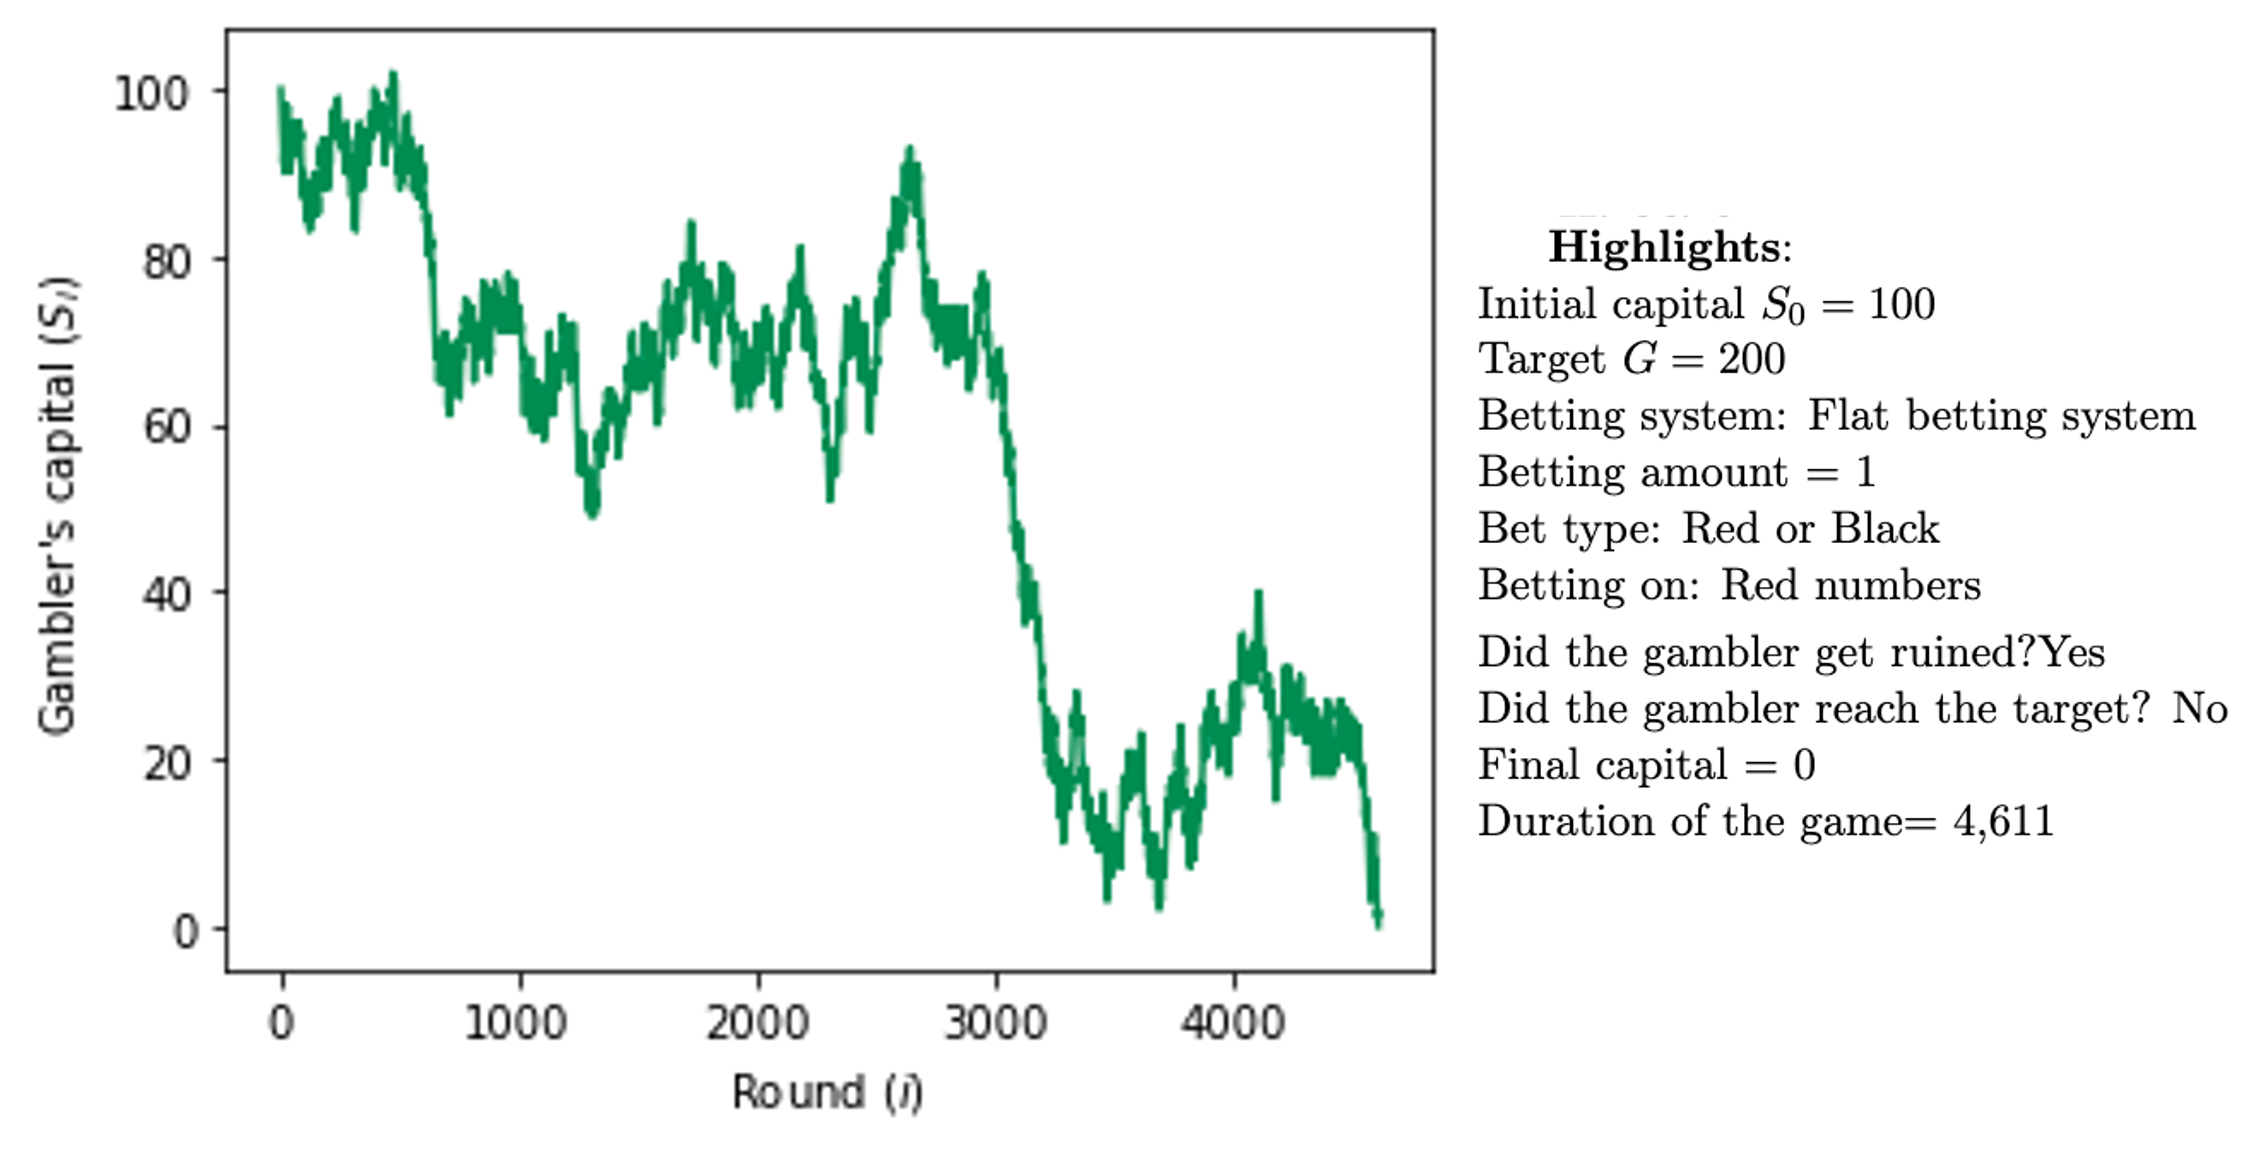
\includegraphics[width=13 cm]{flat_ex_1.png}
        \caption[Flat betting system simulation]{\textit{Flat betting system simulation}. In this simulation, the player started with an initial capital of 100 units and placed bets of 1 unit in each round. The player went bankrupt after playing 4,611 rounds.}\label{sim_01}
\end{figure}

The main advantage of the flat betting strategy is its simplicity and ease of implementation. Also, this strategy is useful for reducing the risk of substantial losses associated with aggressive betting systems when gambler's capital is large enough with respect to bet amount $k$.

However, since betting a fixed amount does not consider the current player's capital ($S_{n}$), it can lead to potential overexposure to risk if the available capital is relative small. Furthermore, this strategy can be considered a conservative approach for reaching profit targets because it may not lead to significant gains in a small or limited number of rounds. In other words, when the target profit is relative huge with respect to the initial capital, the number of rounds to be played increases and may result impractical for the gambler to keep betting until reaching $G$.


\subsection{Proportional betting system}
To address the potential drawbacks of the flat betting system, the proportional betting strategy is introduced. Under this system, the gambler bets a fixed proportion $l$ of their available capital on each round. The bet amount for the $i$th round is given by:
\begin{eqnarray}
     \beta_{i} = lS_{i-1},  & l\in (0,1].
\end{eqnarray}
   
The proportional betting system adapts the bet amount to the changing size of the gambler's capital, ensuring more consistent risk exposure. 

When $l<1$, it is impossible for the player to deplete their capital entirely because a fraction of the player's capital will always remain after each betting round\footnote{To implement this betting strategy in a simulation, it's necessary to define a ruin threshold, denoted as $\epsilon$. This threshold signifies the practical end of the game, represented by the event $\{S_{n} < \epsilon\}$.}. In this scenario, the fixed betting proportion ensures that the player is not risking their entire capital in any single bet. Even in the event of a losing streak, the bet size will decrease proportionally to the declining capital, thus reducing the impact of losses. 

However, the assumption of infinitely divisible capital is an idealization that may not be practical in real-world casinos. In reality, casinos usually have minimum and maximum betting limits, which restrict the amount that a player can wager on each round. 

This strategy has two main drawbacks. First, when the available capital is large, even a small fixed proportion can result in significant bet amounts. This can expose the player to higher risks, especially while betting on low probability options. Large bet amounts may lead to substantial losses in a short period, even if the player is using a conservative proportion
The second disadvantage id the choosing of the parameter $l$. The challenge while using this strategy is to fix the value of $l$. To determine the appropriate value for $l$, gamblers need to consider their risk profile and betting objectives. The choice of $l$ should strike a balance between consistent risk management and the potential for achieving profit targets.

Another important consideration is that under the proportional betting system, the specific initial capital, and profit goal are no longer the primary focus. Instead, the target ratio takes center stage as a critical factor that guides the gambler's strategy. This ratio offers a clear and standardized way for gamblers to define their profit objectives in relation to their starting capital.

\begin{Definition}
    \textbf{Target ratio}. The target ratio is defined as the ratio between the profit target of the gambler $G$ and the initial capital $S_{0}$:
    $$\frac{G}{S_{0}}.$$
When the target ratio is equal to 1, the gambler aims to double their initial capital.
\end{Definition}

Algorithm \ref{alg:2} shows how to simulate one path of the game using the proportional betting system to reach a profit target ($G$). According to this algorithm, each round is determined as a win or a loss based on a calculated winning probability. Then, the gambler's capital is adjusted according to the outcomes of the round (win or loss), then the bet amount is adjusted proportionally to the updated capital. The algorithm continues until either the profit target is reached or the ruin threshold is breached, and it provides the path of the capital throughout the game.

Figure \ref{sim_02} depicts a simulation in which a gambler started with an initial capital of $100$ with a target of $200$ and betting $l =20\%$ of his available capital on the red numbers, in each round. In this game, the player ended with a capital less than $\epsilon = 0.1$ after 147 rounds.
\begin{algorithm}
\caption{Roulette game using a proportional strategy to reach a profit target G.} \label{alg:2}
\SetAlgoLined
\SetKwInOut{Input}{Input}
\SetKwInOut{Output}{Output}

\Input{Profit target $G$, initial capital $z$, payoff $\phi$, ruin threshold $\epsilon$, proportional bet amount $l$}
\Output{Path of the capital $S_{n}$}
$target \gets G$\;
$flag \gets 0$\;
$S_{n} \gets [z]$\;
$bet\_amount \gets lS_{n}[-1]$\;
\While {flag = 0}{
    generate uniformly distributed random number $x \in [0,1]$\;
    \If{$x< \frac{36}{(\phi +1)37}$ }{
        Append $S_n[-1] +\phi \times \text{bet\_amount} $ to $S_n$\;
    }
    \Else{
        Append $S_n[-1] - \text{bet\_amount} $ to $S_n$\;
    }
    $bet\_amount \gets lS_{n}[-1]$\;
    \If{$S_n[-1] \geq \text{target}$ \textbf{or} $S_n[-1] < \epsilon$} {
        flag $\leftarrow$ 1\;
    }
}
\Return $S_{n}$\;
\end{algorithm}

\begin{figure}[H]
        \centering
        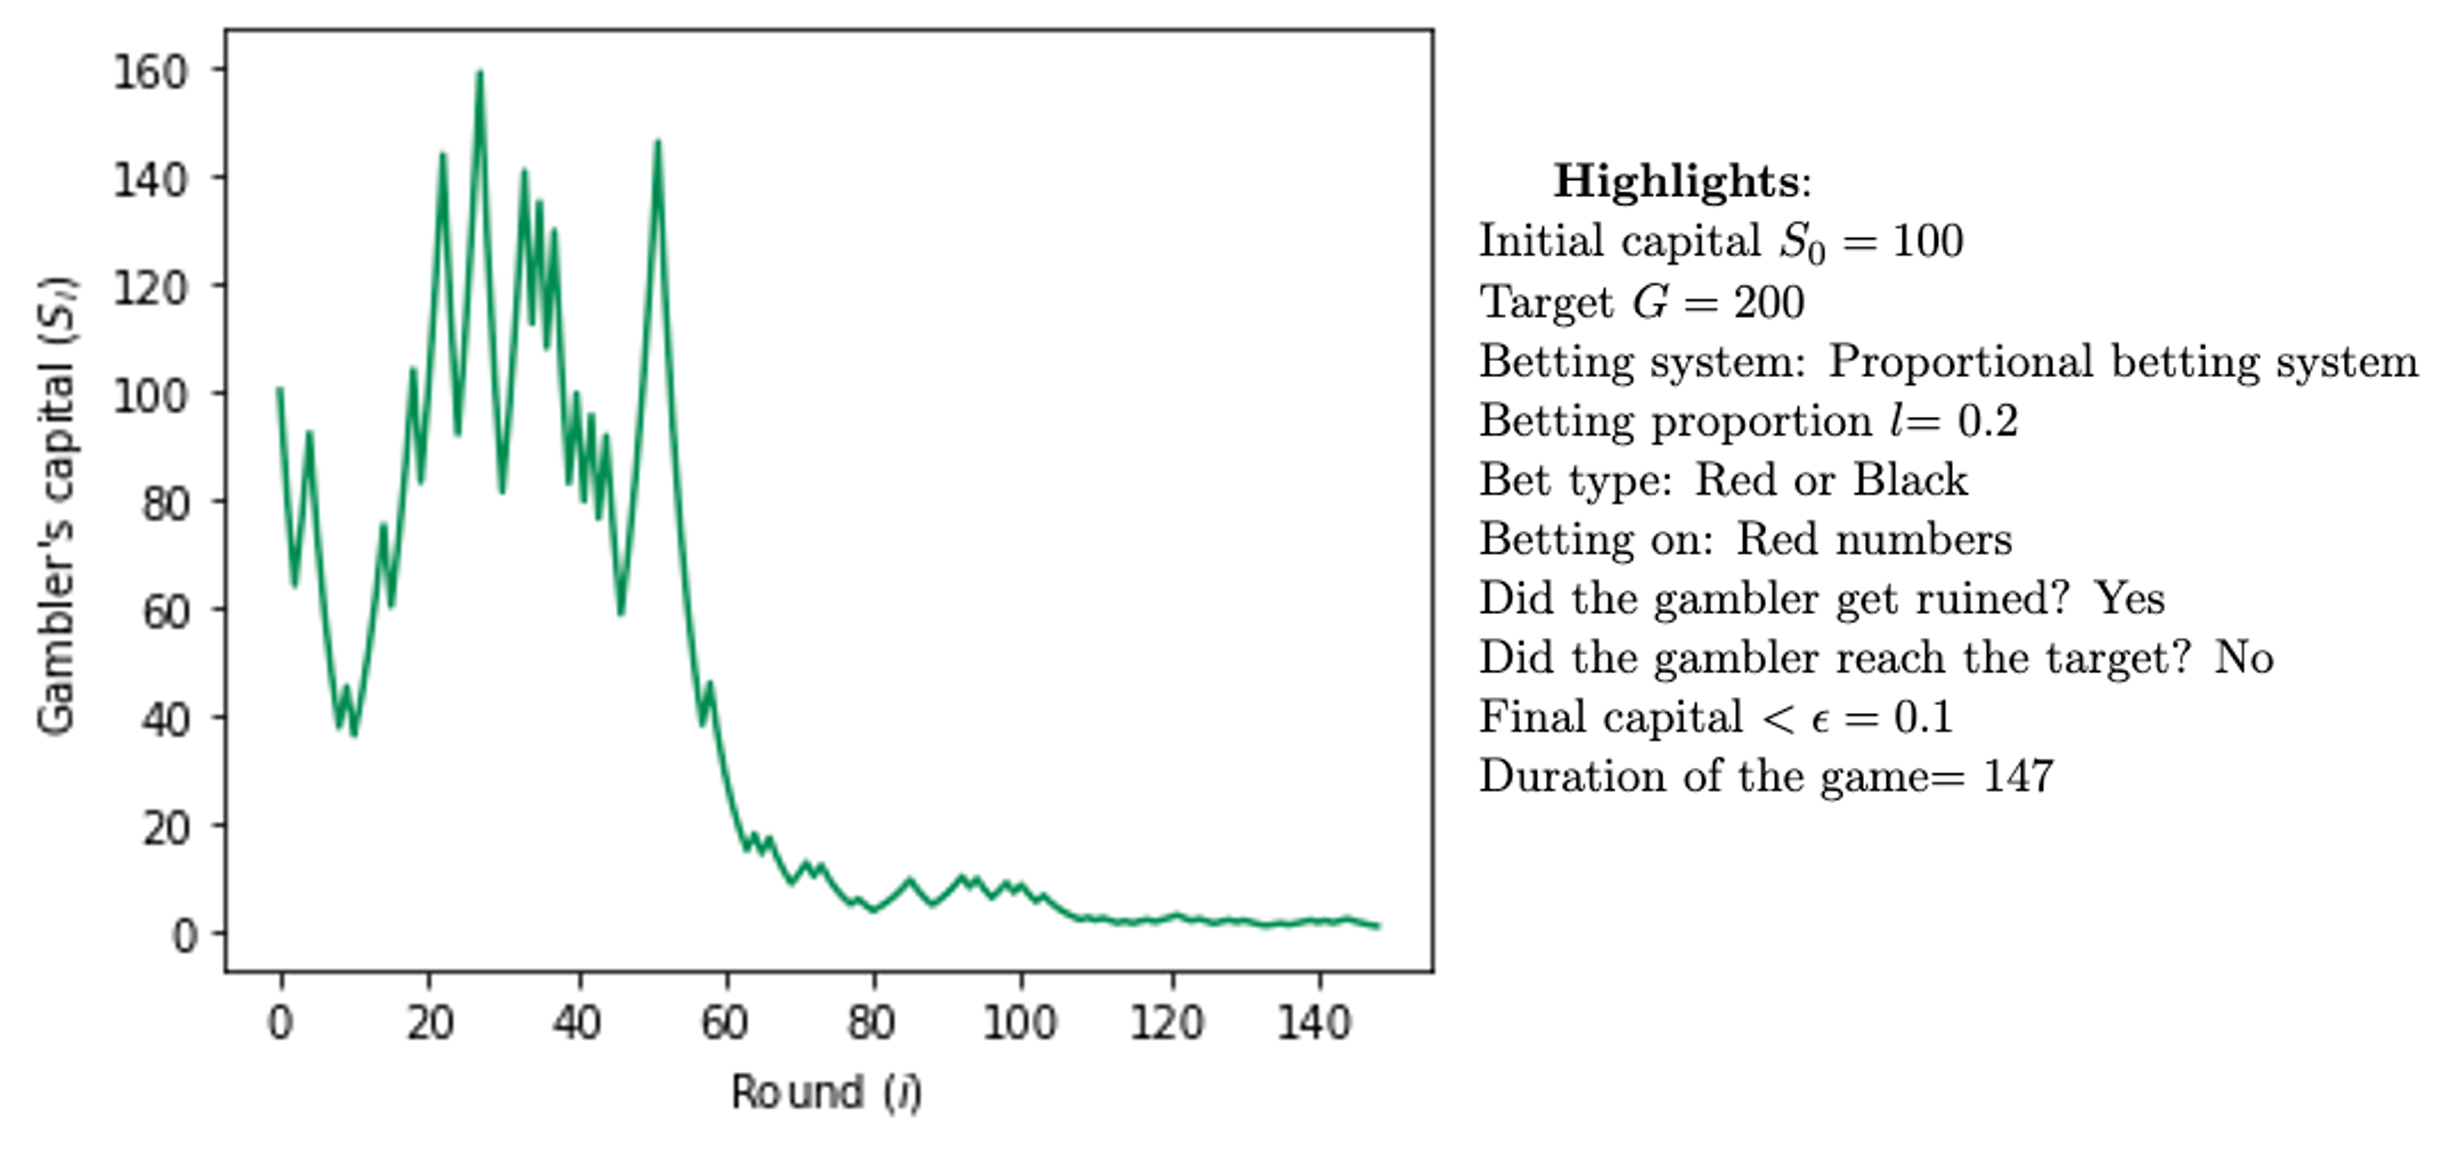
\includegraphics[width=13 cm]{pro_ex_1.png}
        \caption[Proportional betting system simulation]{\textit{Proportional betting system simulation}. In this simulation, the player started with an initial capital of 100 units and bets 20\% of his available capital each round. The player went bankrupt after playing 147 rounds.}\label{sim_02}
\end{figure}
\subsection{Martingale betting system}
In the Martingale system, the betting amount for each round depends on the outcome of the previous round. The goal of this system is to place a bet large enough so in the event of winning, the gambler would not only recover all previous losses but also secure an additional 1 unit as profit. 

The classical martingale strategy is defined for even-money bets and it is also known as doubling or geometric progression procedure. In this case the gambler doubles his bet size after each loss until reach a win:

\begin{equation*}
\beta_{i} = \left\{
\begin{array}{ll}
1 &  i = 1\\
2\beta_{i-1}\1_{\{X_{i-1} = -1\}} &  i\geq 2,
\end{array}
\right.
\end{equation*}

where $X_{i}$ corresponds to the round outcome as defined in (\ref{round_outcome}). Using the recursion, and assuming the gambler consistently places bets on a specific type of bet or uses bet types with the same payoff,  we can rewrite the last expression in terms on the first bet:
\begin{equation}
\beta_{i} = \left\{
\begin{array}{ll}
1 &  i = 1\\
2^{i-1}\1_{\{X_{1} =...=X_{i-1} = -1\}} & i\geq 2.
\end{array}
\right.
\end{equation}

The gambler initiates the betting sequence by placing a wager of 1 unit. If the initial bet results in a win, the gambler receives the payout according to the game's odds and the betting round concludes. However, if the first bet results in a loss, the Martingale strategy comes into play. In response to the loss, the gambler doubles the betting amount for the next round. The purpose of this doubling is to recoup the previous loss and achieve a 1-unit profit when a subsequent win occurs \cite{chances}.

This system can be generalized to a \textit{m-to-1} payout bets as follows:

\begin{equation}\label{mart_1}
\beta_{i} = \left\{
\begin{array}{ll}
\frac{1}{\phi} & i = 1\\
(\frac{1}{\phi} +1)\beta_{i-1}\1_{\{X_{i-1} = -1\}}  &  i\geq 2,
\end{array}
\right.
\end{equation}
where $\phi \geq 1$ is the payout of the type of bet the gambler is using and $X_{i}$ corresponds to the round outcome as defined in (\ref{x_i_ext}). Expression \ref{mart_1} can also be rewritten in terms of the first bet:

\begin{equation}
\beta_{i} = \left\{
\begin{array}{ll}
\frac{1}{\phi}  & i = 1\\
\frac{1}{\phi}(\frac{1}{\phi} +1)^{i-1}\1_{\{X_{1} =...=X_{i-1} = -1\}} &  i\geq 2.\label{mart_bet}\\
\end{array}
\right.
\end{equation}

While the successive amounts bet are dependent on the previous outcomes, the final result of a win or loss in a game of chance remains independent of the bet amounts. 

According to (\ref{mart_bet}), as losses accumulate, the bet size grows exponentially, leading to large and potentially unsustainable bets. A series of losses can quickly consume the gambler's bankroll.\\

The Martingale system relies on the assumption that a win will eventually occur, and the player will recoup all losses plus a profit. However, there are limitations to this strategy. Many casinos have table limits, which restrict the maximum bet that can be placed. When using the martingale system, reaching the table limit can prevent the player from recovering losses even after a winning bet. Furthermore, to implement the martingale system effectively, the player needs a considerable capital to withstand a streak of losses. \\

Ethier \cite[P.99]{chances} gives the following conclusion about this strategy:
\begin{quote} 
{\fontfamily{qpl}\selectfont
This is an infallible system. The difficulty is that, after a sufficiently long sequence of losses, the system will call for a bet that either exceeds what is left to the gambler's resources or exceeds the house maximum betting limit. In either case, the system must be aborted.}
\end{quote}


Algorithm \ref{alg:3} shows how to simulate one path of the game using the Martingale strategy to reach a profit target ($G$). The algorithm operates through a series of rounds, each of which concludes with either a win or a loss. The outcome of each round is determined by a calculated winning probability. The algorithm adapts the betting amount in correspondence with the round's outcome. Specifically, the betting amount is set as $1/ \phi$ after a win or during the first round. However, after a loss, the bet amount is adjusted to a value that would not only recover the accumulated losses but also yield a net gain of 1 unit in case of a win.

The process iterates until one of two conditions is satisfied: the profit target $G$ is reached, or the player's capital diminishes to an amount lower than the current bet amount. 
\clearpage

\begin{algorithm}
\caption{Roulette game using the Martingale strategy to reach a profit target G.}\label{alg:3}
\SetAlgoLined
\SetKwInOut{Input}{Input}
\SetKwInOut{Output}{Output}

\Input{Profit target $G$, initial capital $z$, payoff $\phi$}
\Output{Path of the capital $S_{n}$}
$target \gets G$\;
$bet\_amount \gets 1/ \phi$\;
$flag \gets 0$\;
$S_{n} \gets [z]$\;
$loss \gets 0$\;
\While {flag = 0}{
    generate uniformly distributed random number $x \in [0,1]$\;
    \If{$x< \frac{36}{(\phi +1)37}$ }{
        Append $S_n[-1] +\phi \times \text{bet\_amount} $ to $S_n$\;
        $loss \gets 0$\;
        $bet\_amount \gets 1/ \phi$\;
    }
    \Else{
        Append $S_n[-1] - \text{bet\_amount} $ to $S_n$\;
        $loss \gets loss + \text{bet\_amount}$\;
        $bet\_amount \gets (loss +1)/\phi$\;
    }
    \If{$S_n[-1] \geq \text{target}$ \textbf{or} $S_n[-1] < \text{bet\_amount}$} {
        flag $\leftarrow$ 1\;
    }
}
\Return $S_{n}$\;
\end{algorithm}

Figure \ref{sim_03} depicts a simulation of the Martingale betting system in which the initial capital is $100$, the target $G = 200$ and the gambler consistently bets on the red numbers. In this simulated path, the gambler finished the game with a capital of $44$ but he could not reach the goal, since the requested bet amount was higher than the available capital in round $140$. As this case depicts, the gambler was neither ruined nor successful reaching $G$.

\begin{figure}[H]
        \centering
        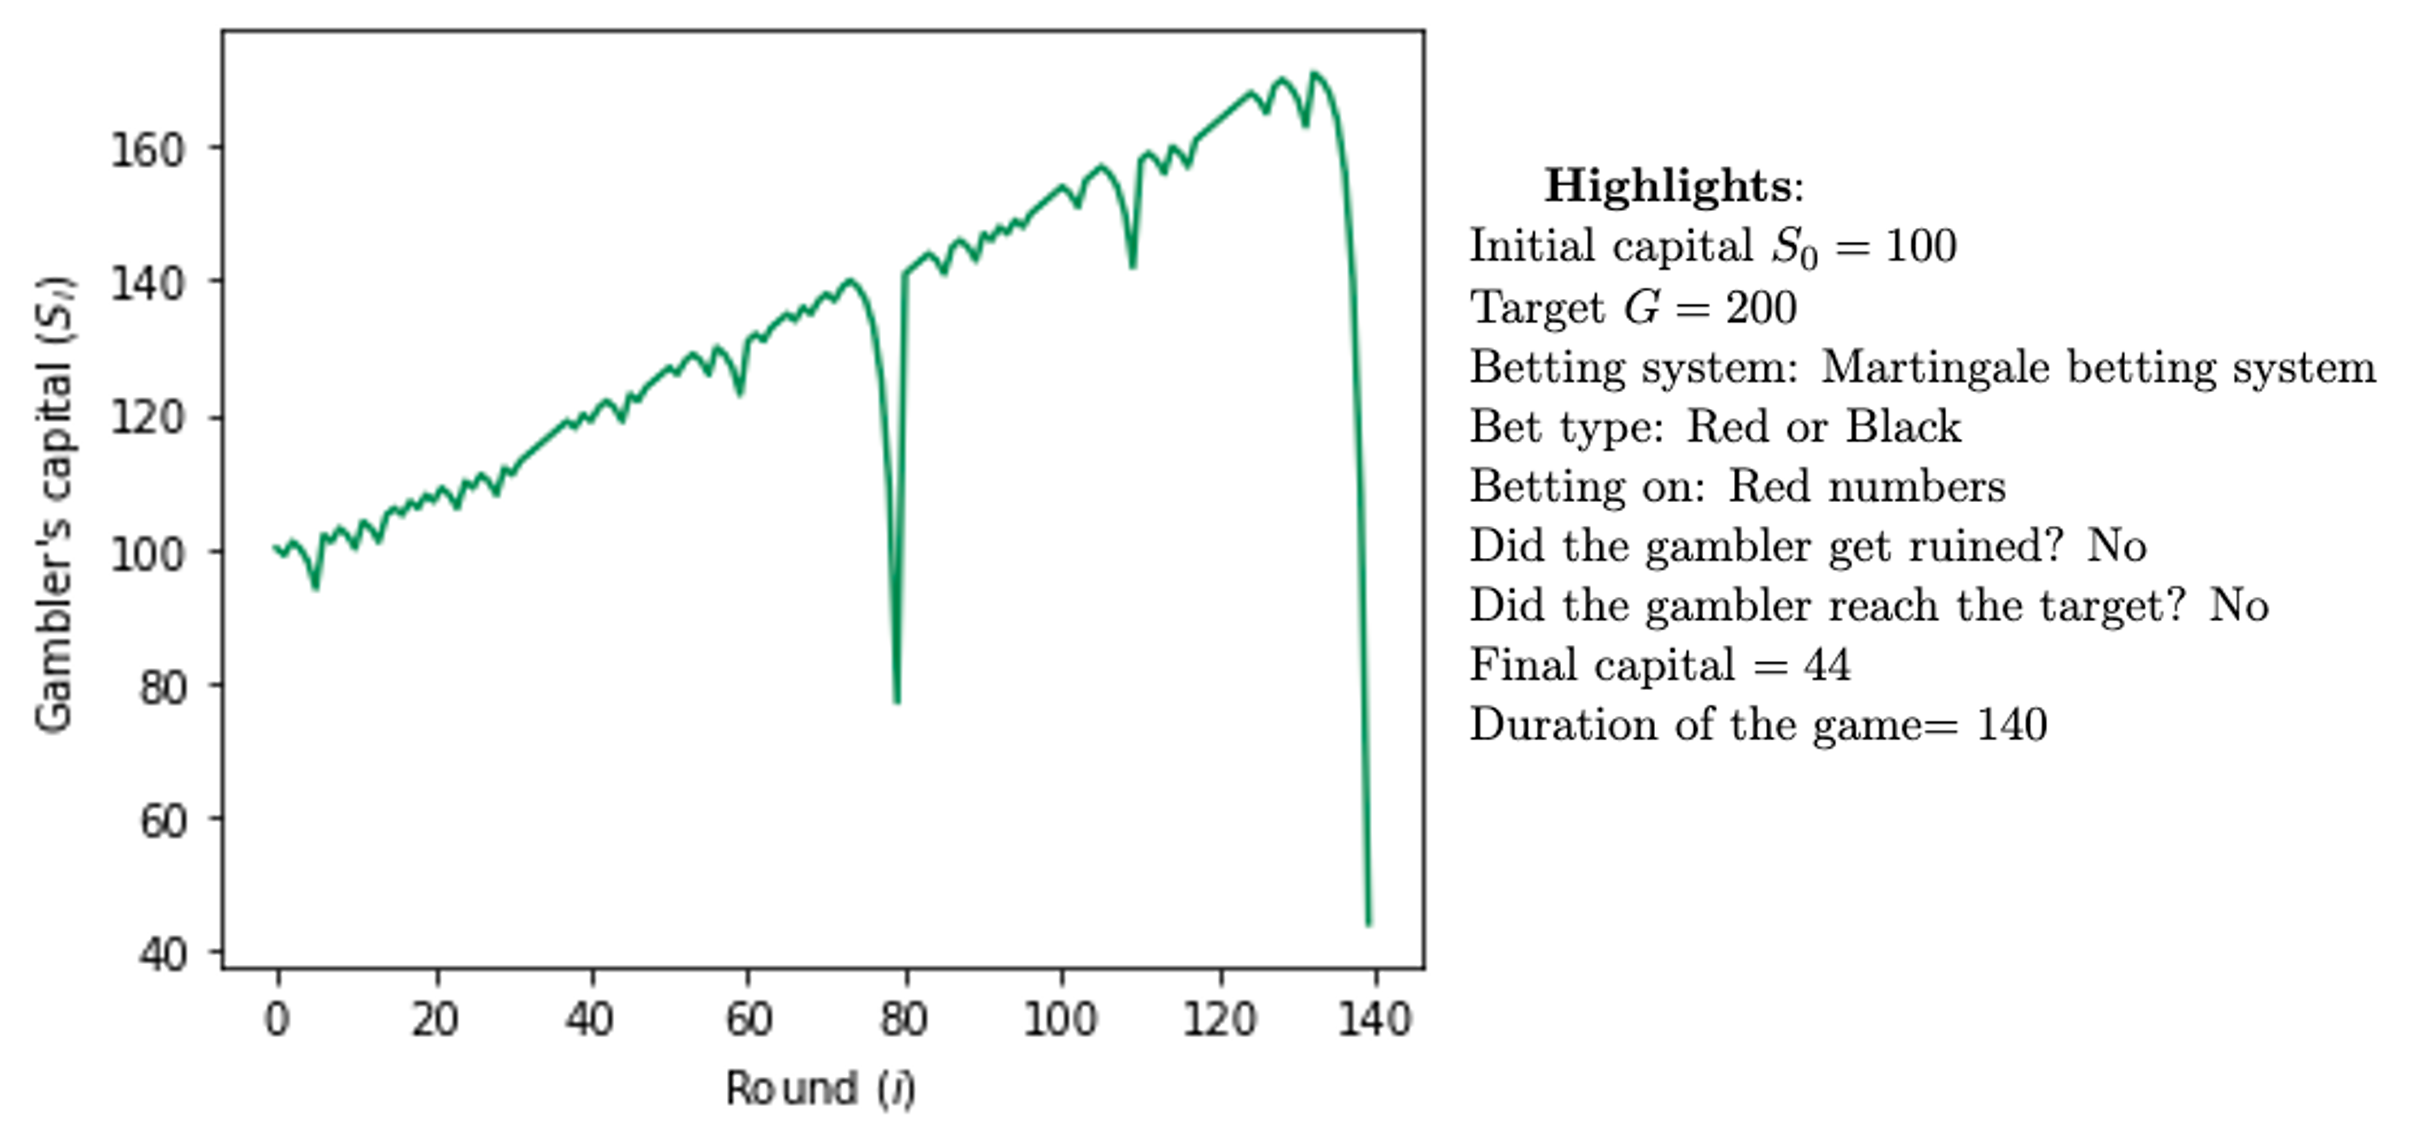
\includegraphics[width=13 cm]{mart_ex_1.png}
        \caption[Martingale betting system simulation]{\textit{Martingale  betting system simulation}. In this simulation, the player started with an initial capital of 100 units. The player could not keep betting since the available capital $44$, was not enough to place the bet amount required by the strategy.}\label{sim_03}
\end{figure}


\subsection{Risk adaptable betting system}

Players aiming to attain specific profit targets often instinctively adjust their betting strategies over time following this rationale: Initially, they might embrace higher-risk wagers to rapidly accumulate significant capital, leveraging the higher payoff for substantial gains. In the early stages, with limited capital at stake, they exhibit a greater tolerance for risk, driven by the belief that potential rewards outweigh potential losses. However, as they approach their profit goal, their focus shifts toward safeguarding their gains. The psychological satisfaction of nearing the profit target intensifies their aversion to potential losses, prompting a preference for more cautious bets. This shift is intended to conserve their progress and solidify their success.

Under a risk adaptable approach, or a mixed-risk strategy, gamblers initially engage in higher-risk bets. As their capital increases, they transition to safer bets characterized by higher winning probabilities (and comparatively smaller payouts). This strategic evolution aims to protect the capital they have accumulated while maximizing their chances of overall success. Let's consider an example within the context of roulette. Instead of consistently placing high-risk bets on single numbers, a player might opt to bet on a specific dozen or on a group of 4 numbers, as he holds more capital. This natural adaptation is a reflection of his desire to balance risk and reward as his gambling experience evolves.

The proposed risk adaptable strategy combines a proportional betting approach with a range of betting types available in the game. It allows gamblers to modify their betting strategy based on the capital they have and their progress towards their profit target. This strategy is characterized by the following elements:
\begin{itemize}
    \item $G$: Profit target,
    \item $l$: Proportion of available capital to be bet,
    \item $B_{1}, B_{2}, ..., B_{m}$: Bet types sorted from the riskier to the more conservative one, and
    \item $0 <\alpha_{1}< \alpha_{2}<,...,<\alpha_{m-1}<1$: Proportion of the target at which the gambler changes the bet type (milestones).
The betting strategy is as follows:    
\end{itemize}
\begin{equation}
\beta_{i} = lS_{i-1}, \text{ betting on }\left\{
\begin{array}{ll}
\text{Highest risk bet type }B_{1}  & \text{ if }S_{i-1} < \alpha_{1}G\\
\text{Bet type }B_{2} & \text{ if } \alpha_{1}G \leq S_{i-1} < \alpha_{2}G\\
\vdots & \\
\text{Bet type }B_{j} & \text{ if } \alpha_{j-1}G \leq S_{i-1} < \alpha_{j}G\\
\vdots & \\
\text{Lowest risk bet type } B_{m} & \text{ if }\alpha_{m-1}G \leq  S_{i-1}.
\end{array}
\right.
\end{equation}

The bet amount for each round is determined by the proportional betting approach. The choice of bet type, however, is based on the current capital and its relation to predefined milestones. 

The risk adaptable strategy proposed here introduces the concept of milestones. These are predefined levels ($\alpha_{1}, \alpha_{2},...,\alpha_{m-1}$) of capital relative to the profit target $G$. The strategy dictates that as the player's capital crosses each milestone, they change the bet type he is betting on. Higher-risk bets are initially favored to capitalize on the potential for rapid capital growth. However, as the player's capital approaches each milestone, they transition to more conservative bet types to safeguard their progress. The relationship between the milestones, $\alpha_{j}$ is crucial for determining when the player transitions from one phase to another. The specific values of $\alpha_{j}, j \in \{1,...,m-1\}$ depend on the player's risk tolerance, profit goal, and individual strategy.

Figure \ref{adaptable} depicts a diagram of the risk adaptable betting phases for $m = 3$, that is when the bet types can be classified as high, medium and low risk.

\begin{figure}[H]
        \centering
        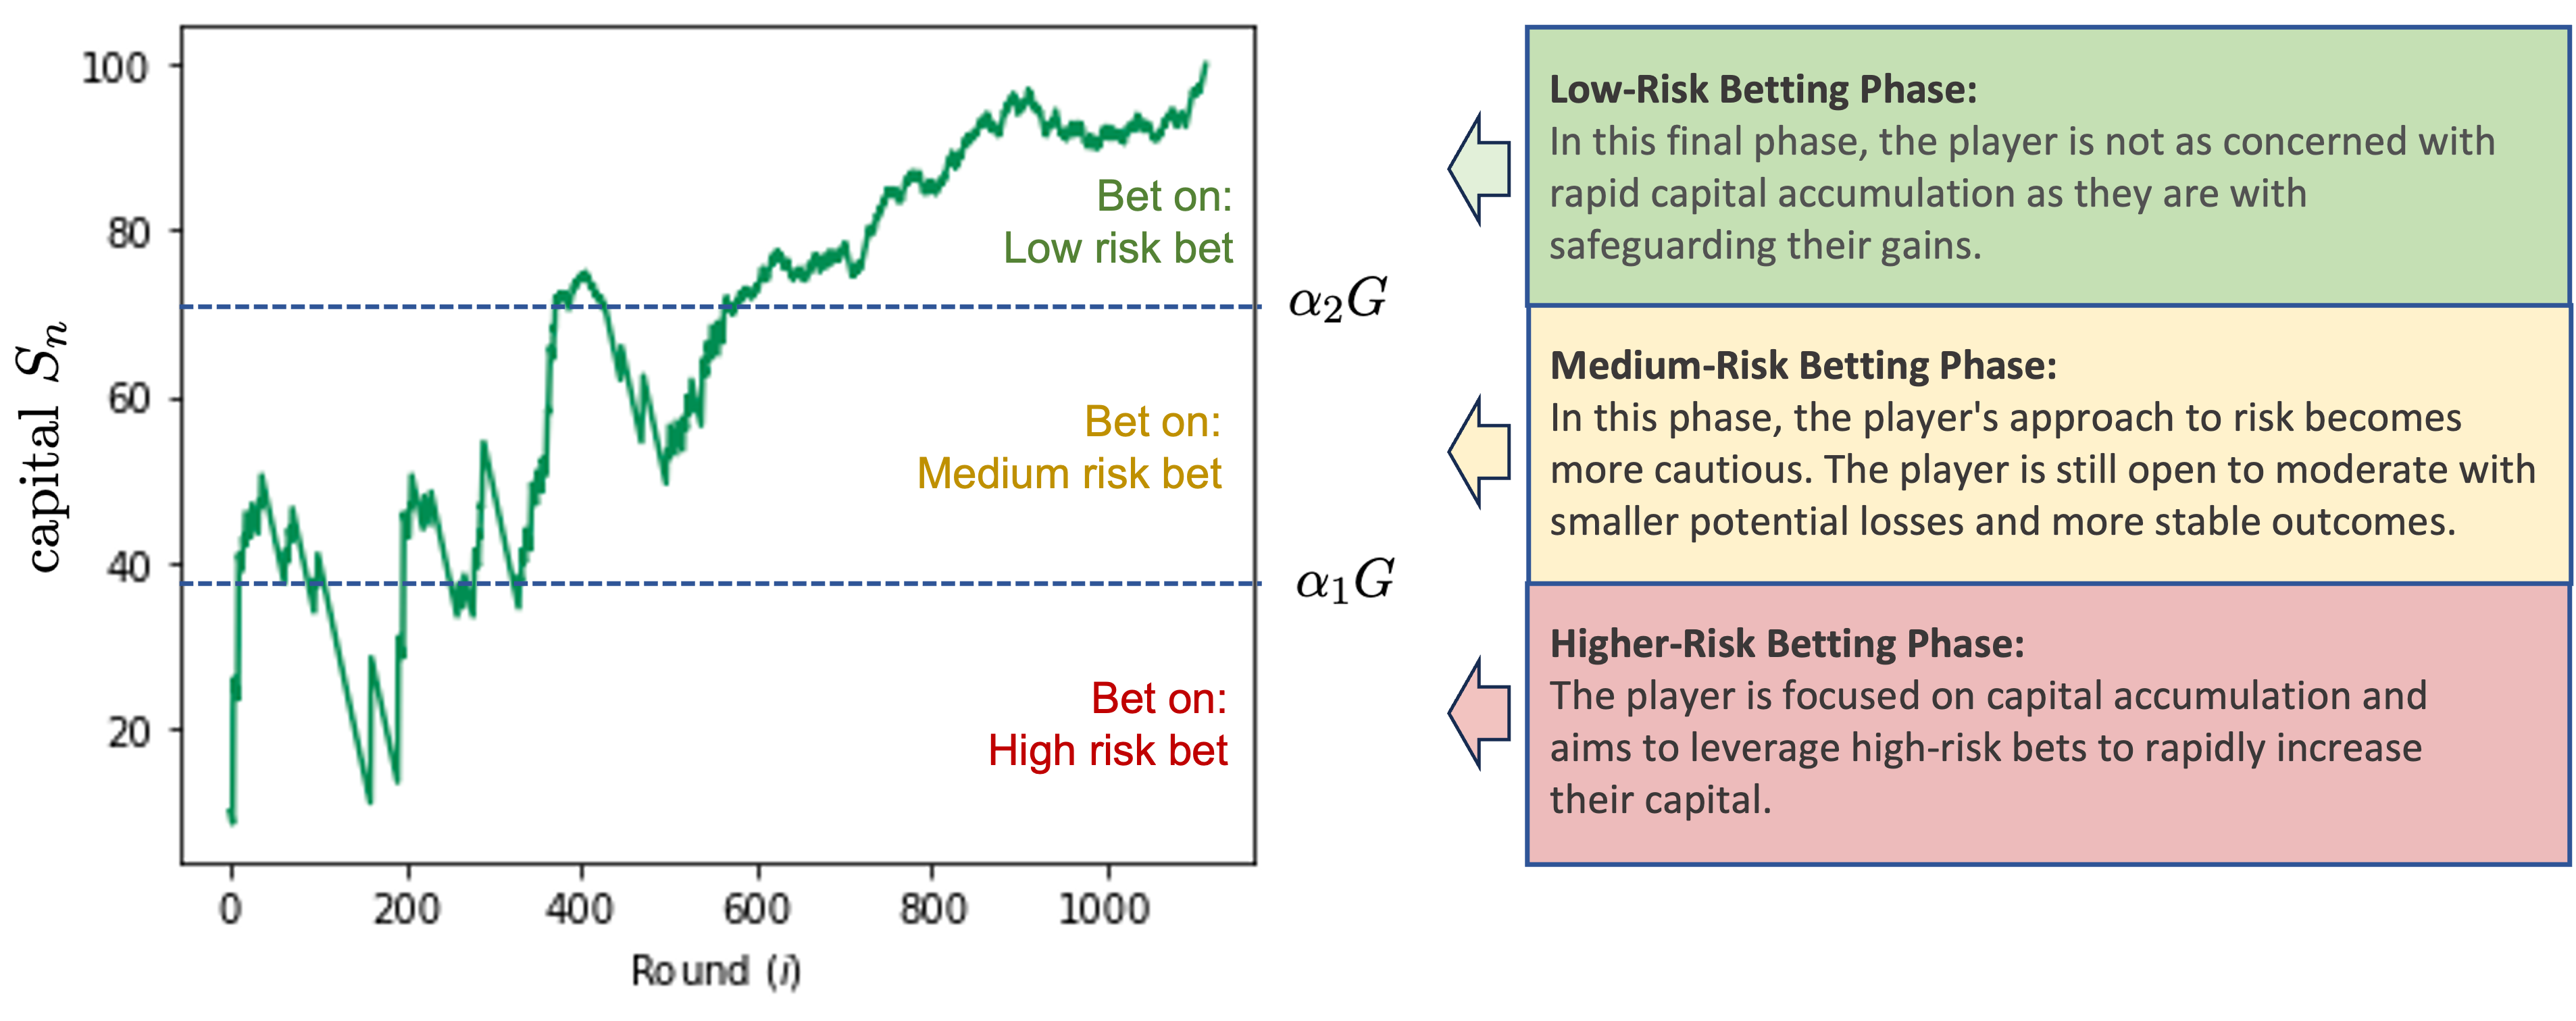
\includegraphics[width=16cm]{risk_adaptable_phases.png}
        \caption[Risk adaptable betting phases diagram]{\textit{Risk adaptable betting phases diagram}. Milestones define critical points in the player's journey towards their profit goal, guiding his shift from risk-taking to risk-averse bet options.}\label{adaptable}
\end{figure}

Consider the payoffs associated with the different bet types, represented as $\phi_{1},..., \phi_{m}$. These payoffs are inherently linked to the risk levels of the bets. Basically, the greater the risk associated with a particular bet, the higher the potential payoff.  When applying the risk adaptable strategy, as depicted in Figure \ref{sim_mixed_22}, a distinct pattern emerges in the dynamics of the gambler's capital. During the initial and riskiest phase of this strategy, the trajectory of the capital showcases pronounced spikes, each magnified by the factor $\phi_{1}$ (the highest of the payoffs). These spikes signify periods of rapid capital growth. However, it's important to recognize that these substantial payoffs are matched with relatively modest bet amounts ($lS_{i}$), primarily due to the comparably lower capital during this phase.

As the player's capital grows and advances closer to the profit goal, the jumps in the capital exhibit a different behaviour because in case of wins, the gambler get lower payoffs. Although the magnitude of the jumps diminishes, it's noteworthy that the accompanying bet amounts rise in proportion.
\begin{figure}[H]
        \centering
        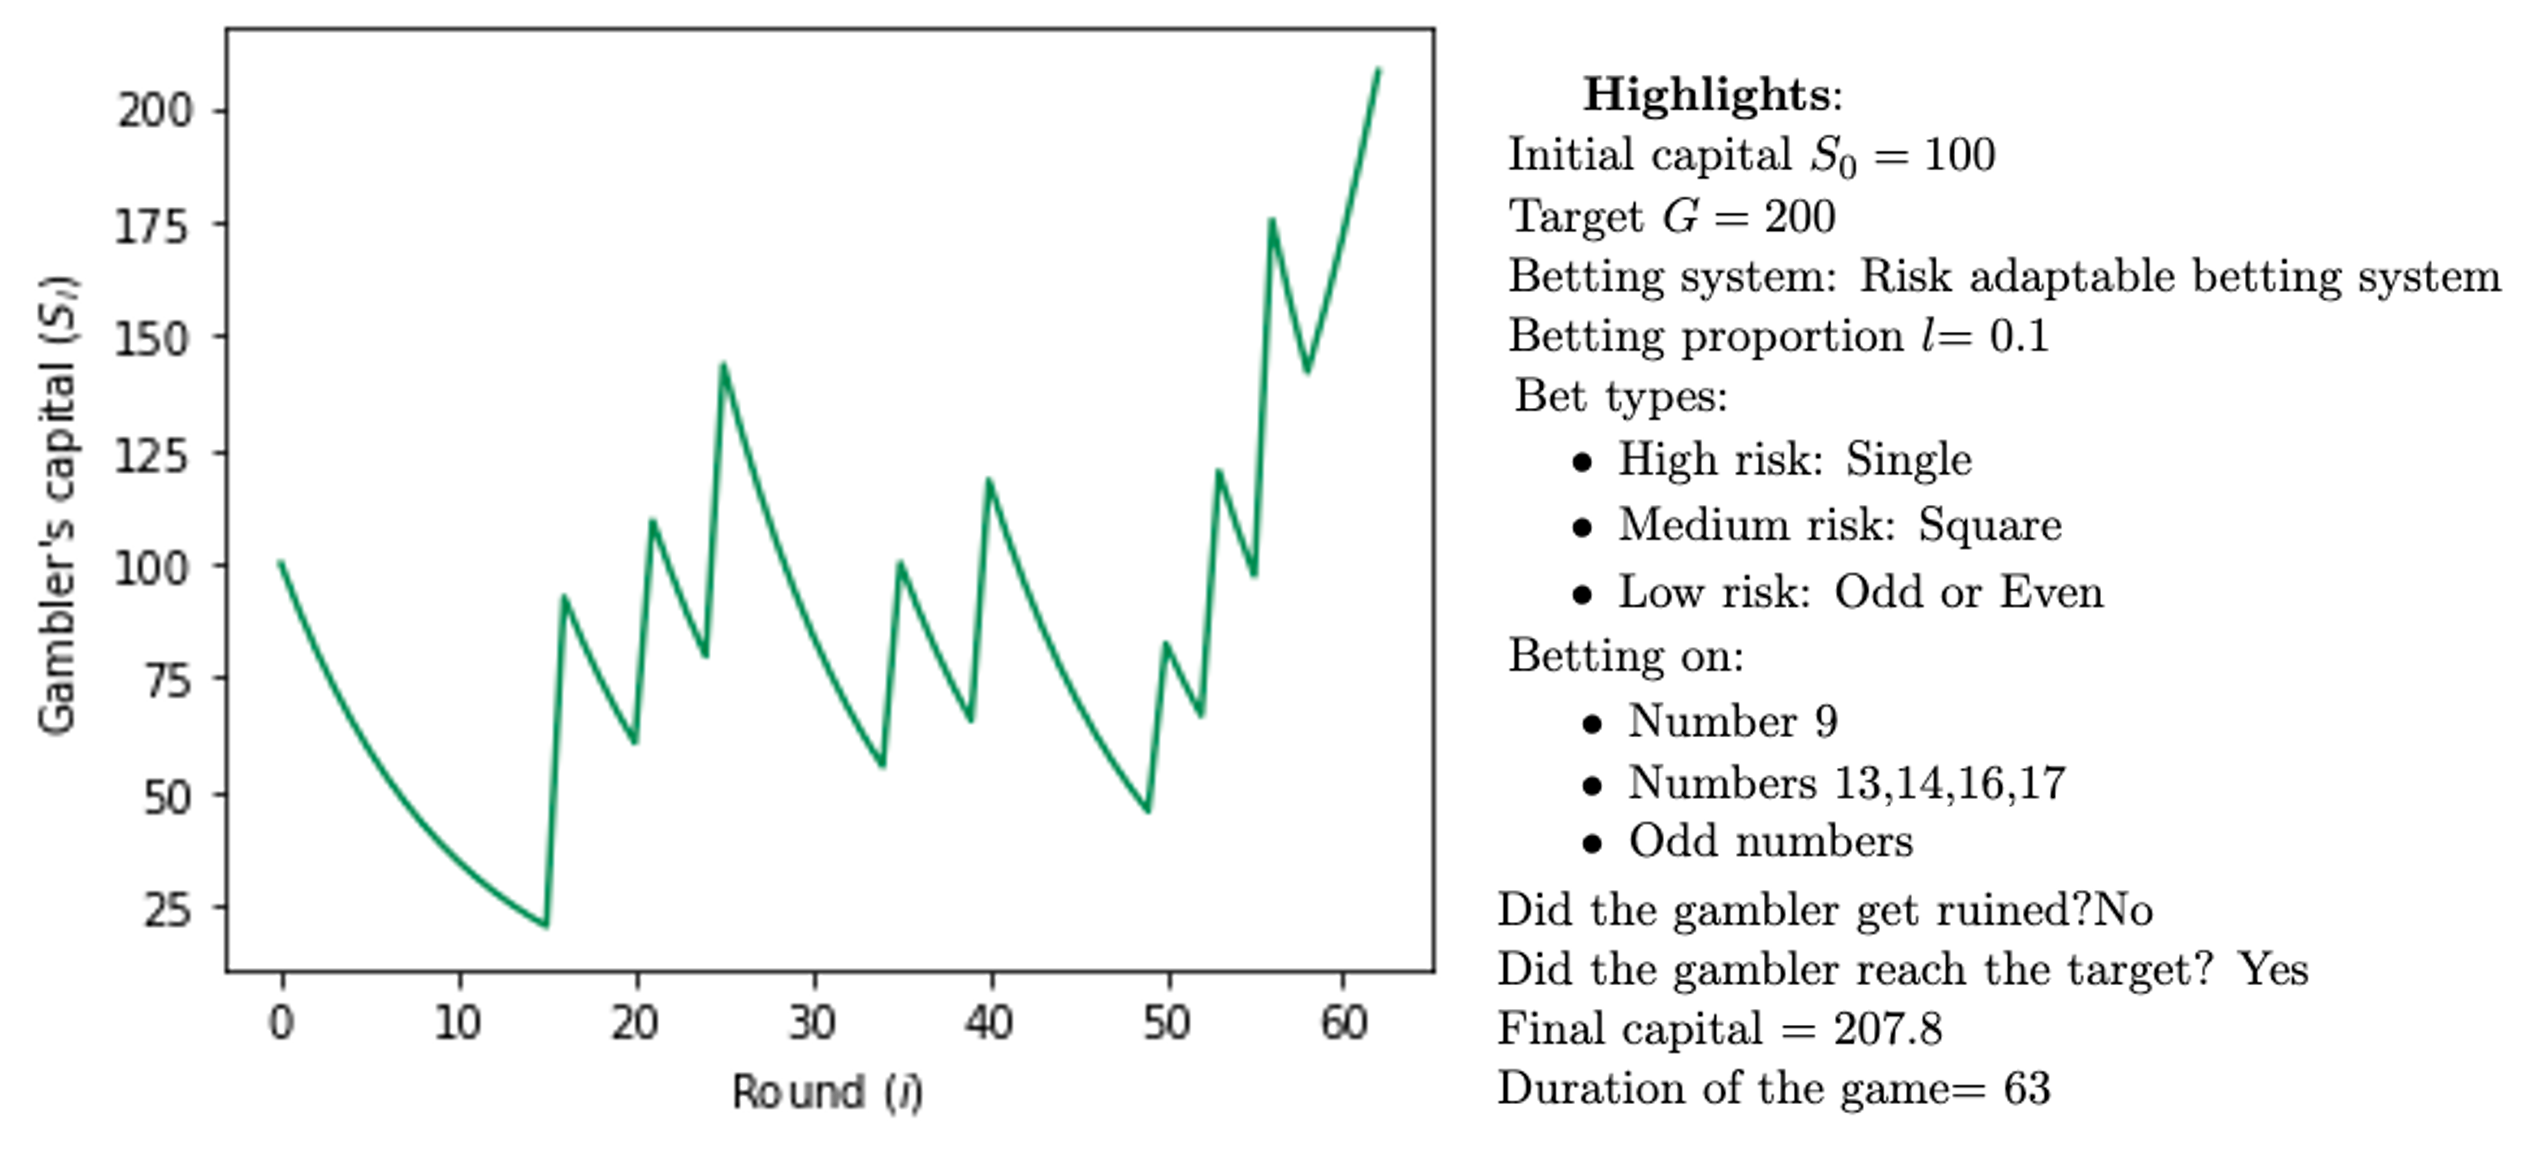
\includegraphics[width=13cm]{mixed_ex_1.png}
        \caption[Risk adaptable betting system simulation]{\textit{Risk adaptable betting system simulation}. In this simulation, the player started with an initial capital of 100 units. The player reach the goal after playing 63 rounds.}\label{sim_mixed_22}
\end{figure}

One of the advantages of this strategy is its emphasis on capital preservation. By incorporating the concept of milestones, players can strategically shift to safer bets with smaller payoffs as their capital approaches and exceeds specific milestones. This approach minimizes the potential for substantial losses, helping players maintain a more consistent capital base over time. However, a potential drawback of the strategy is the subjective nature of selecting appropriate values for the milestones. The effectiveness of the strategy hinges on accurately defining these milestone levels. 

\clearpage
\section{Empirical analysis of betting systems}\label{Empirical_analysis}
This chapter is structured into two parts, each offering a distinct perspective on the performance of the presented betting strategies.

The first part explores some simulations conducted to assess the effectiveness of different betting strategies, using data from the Smart Live Casino. The simulations create hypothetical scenarios illustrating potential outcomes and trajectories based on specific strategies. While not predictive of future results, these simulations serve as a powerful tool to evaluate the relative strengths and weaknesses of different strategies, enabling informed decision-making by gamblers.

The second part of this chapter focuses on the simulation of European roulette spins to compare the outcomes of different betting strategies under two exercises. The first exercise involves strategies that aim to win one monetary unit of capital per round, while the second exercise examines strategies that bet a fixed proportion of available capital in each round.
\subsection{Testing Betting Strategies with Smart Live Casino Data}
By using data from the Smart Live Casino, the following scenarios showcase potential outcomes and trajectories based on specific strategies. While not indicative of future results, these simulations offer a hypothetical view of how strategies might have fared under certain conditions. These examples serve as a tool for assessing the relative strengths and weaknesses of different strategies.
\subsubsection{Flat Betting System}
The first example is the simplest. Let's consider a gambler with an initial capital of $S_{0} = 1000$ who employs the flat betting system with a betting amount of 1 unit. Let's assume that the gambler consistently places bets on the red numbers. Figure \ref{sim_live_01} depicts the gambler's capital $S_{i}$ over the course of the played rounds.

\begin{figure}[H]
    \centering
    \includegraphics[width=11 cm]{sim_01.png}
    \caption[Smart Live Casino - Example 1: Flat Betting System]{\textit{Smart Live Casino - Example 1: Flat Betting System}. The gambler consistently bets 1 unit on the red numbers. After 5,550 rounds, his capital amounted to $S_{5,550} = 908$.}\label{sim_live_01}
\end{figure}

In this example, the bettor participated in 5,550 rounds\footnote{Recall that the Smart Live Casino dataset includes 5,550 spin observations.} until the roulette observations concluded. As a result, their capital stood at $S_{5,550} = 908$, indicating a loss of 92 units in general terms.

Based solely on the observation of example 1, one might be inclined to think that the gambler should have wagered on the black numbers rather than the red ones. The same experiment was conducted with the identical initial capital and bet amount, but this time, bets were placed on the black numbers (see Figure \ref{sim_live_02}). The results reveal that the bettor played the same 5,550 rounds, but concluded with a final capital of $S_{5,550} = 800$. In general terms, this represents a loss of 200 units.

\begin{figure}[H]
    \centering
    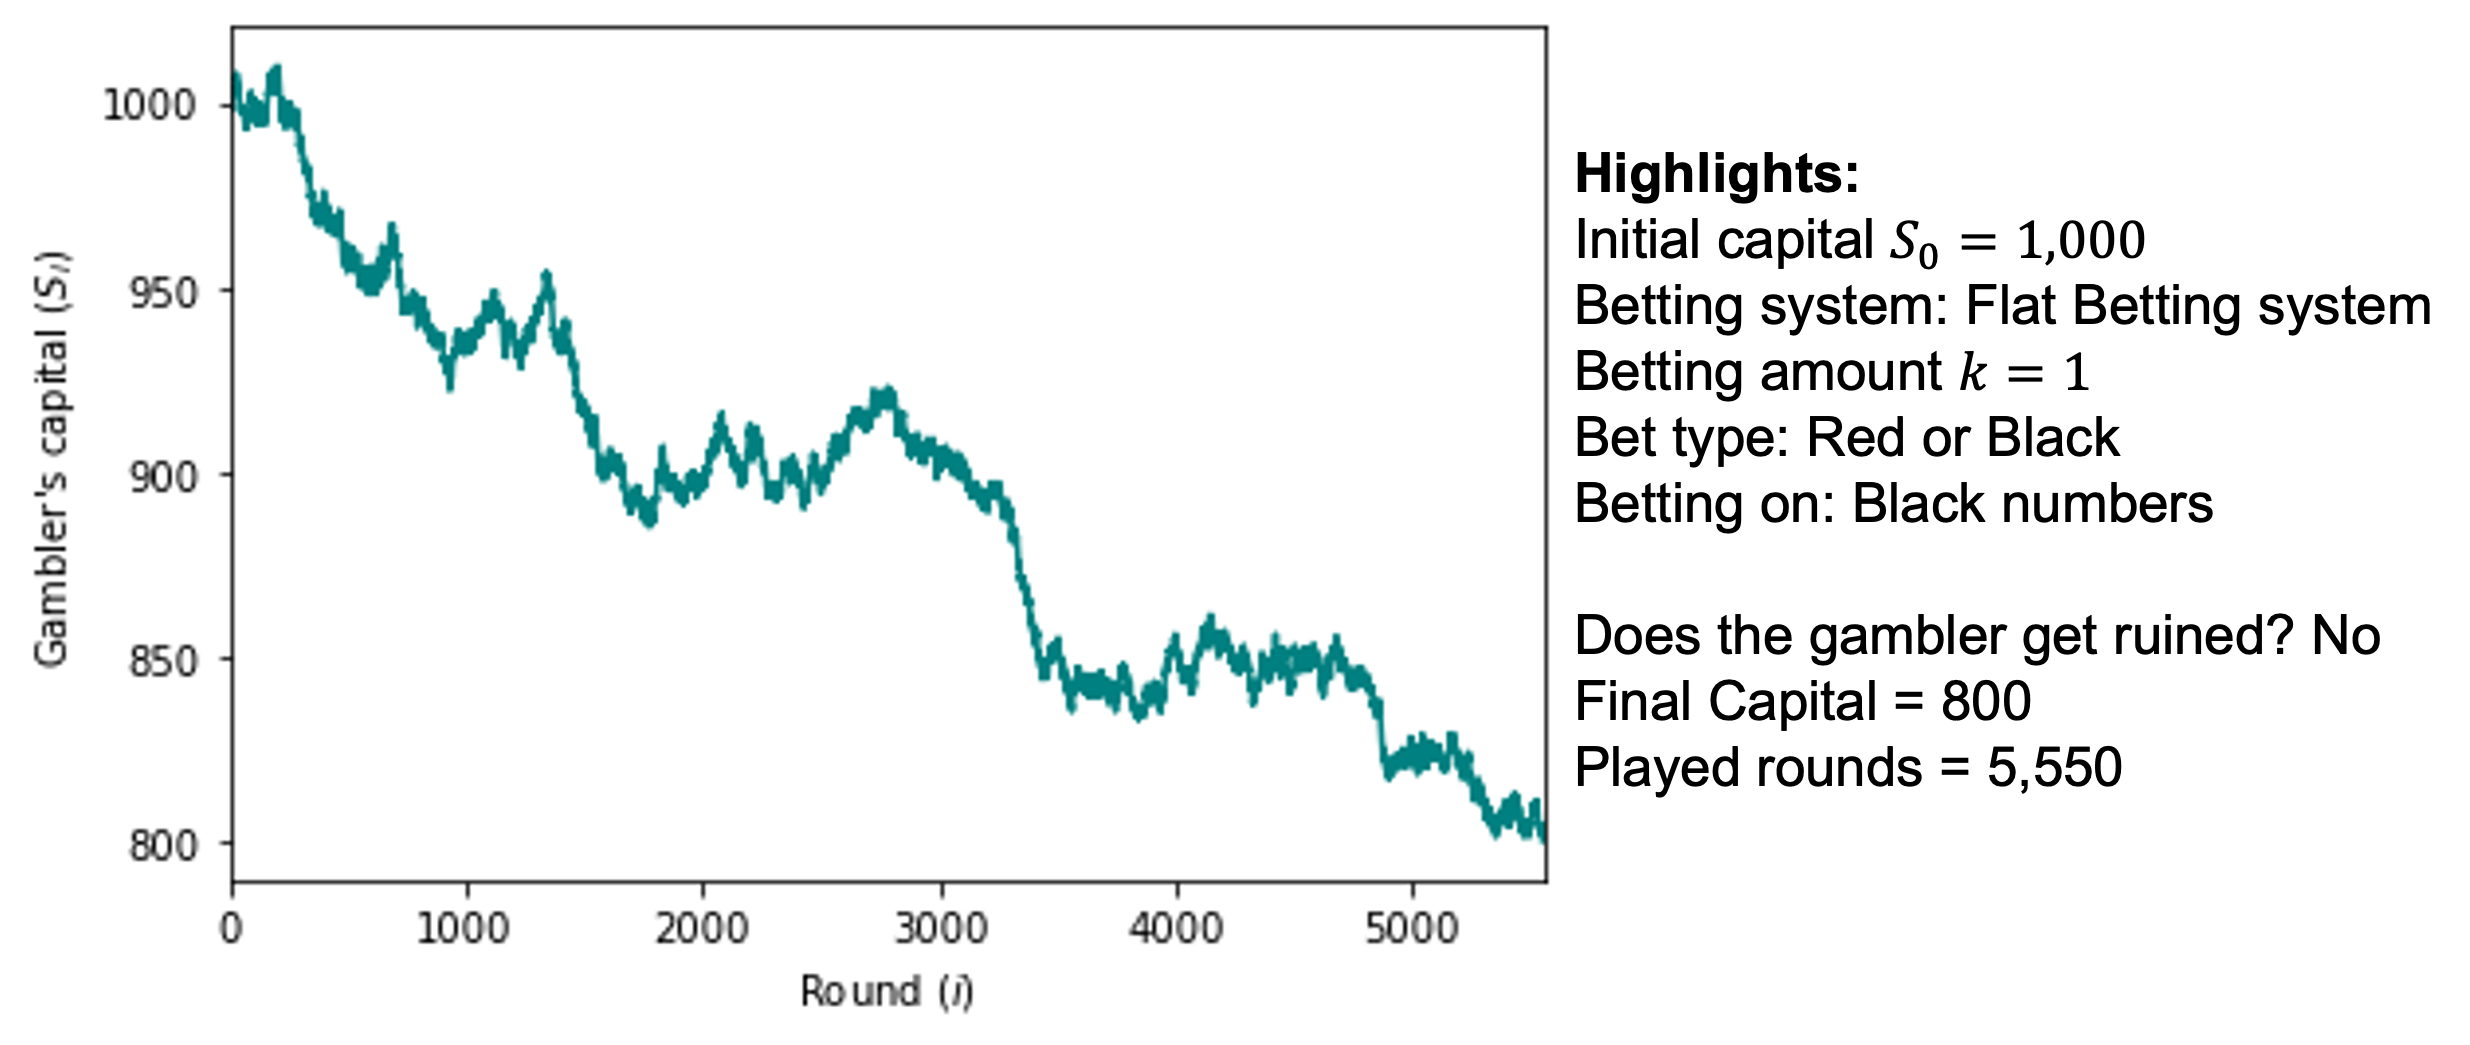
\includegraphics[width=11 cm]{sim_02.png}
    \caption[Smart Live Casino - Example 2: Flat Betting System]{\textit{Smart Live Casino - Example 2: Flat Betting System}. The gambler consistently bets 1 unit on the black numbers. After 5,550 rounds, their capital amounted to $S_{5,550} = 800$. }\label{sim_live_02}
\end{figure}
In both examples 1 and 2, the gambler concluded with a final capital smaller than the initial capital due to the house advantage. This demonstrates that the house always maintains an edge over the players, regardless of whether the gambler places bets on black or red numbers.

By adjusting the betting amount, the duration of the game can  significantly change. Example 3 is an extension of example 2 in which the betting amount increases from 1 to 10 units. In this scenario, the gambler participated in only 1,569 rounds before facing ruin. The path of the gambler's capital $S_{i}$ over the rounds is illustrated in Figure \ref{sim_live_03}:

\begin{figure}[H]
    \centering
    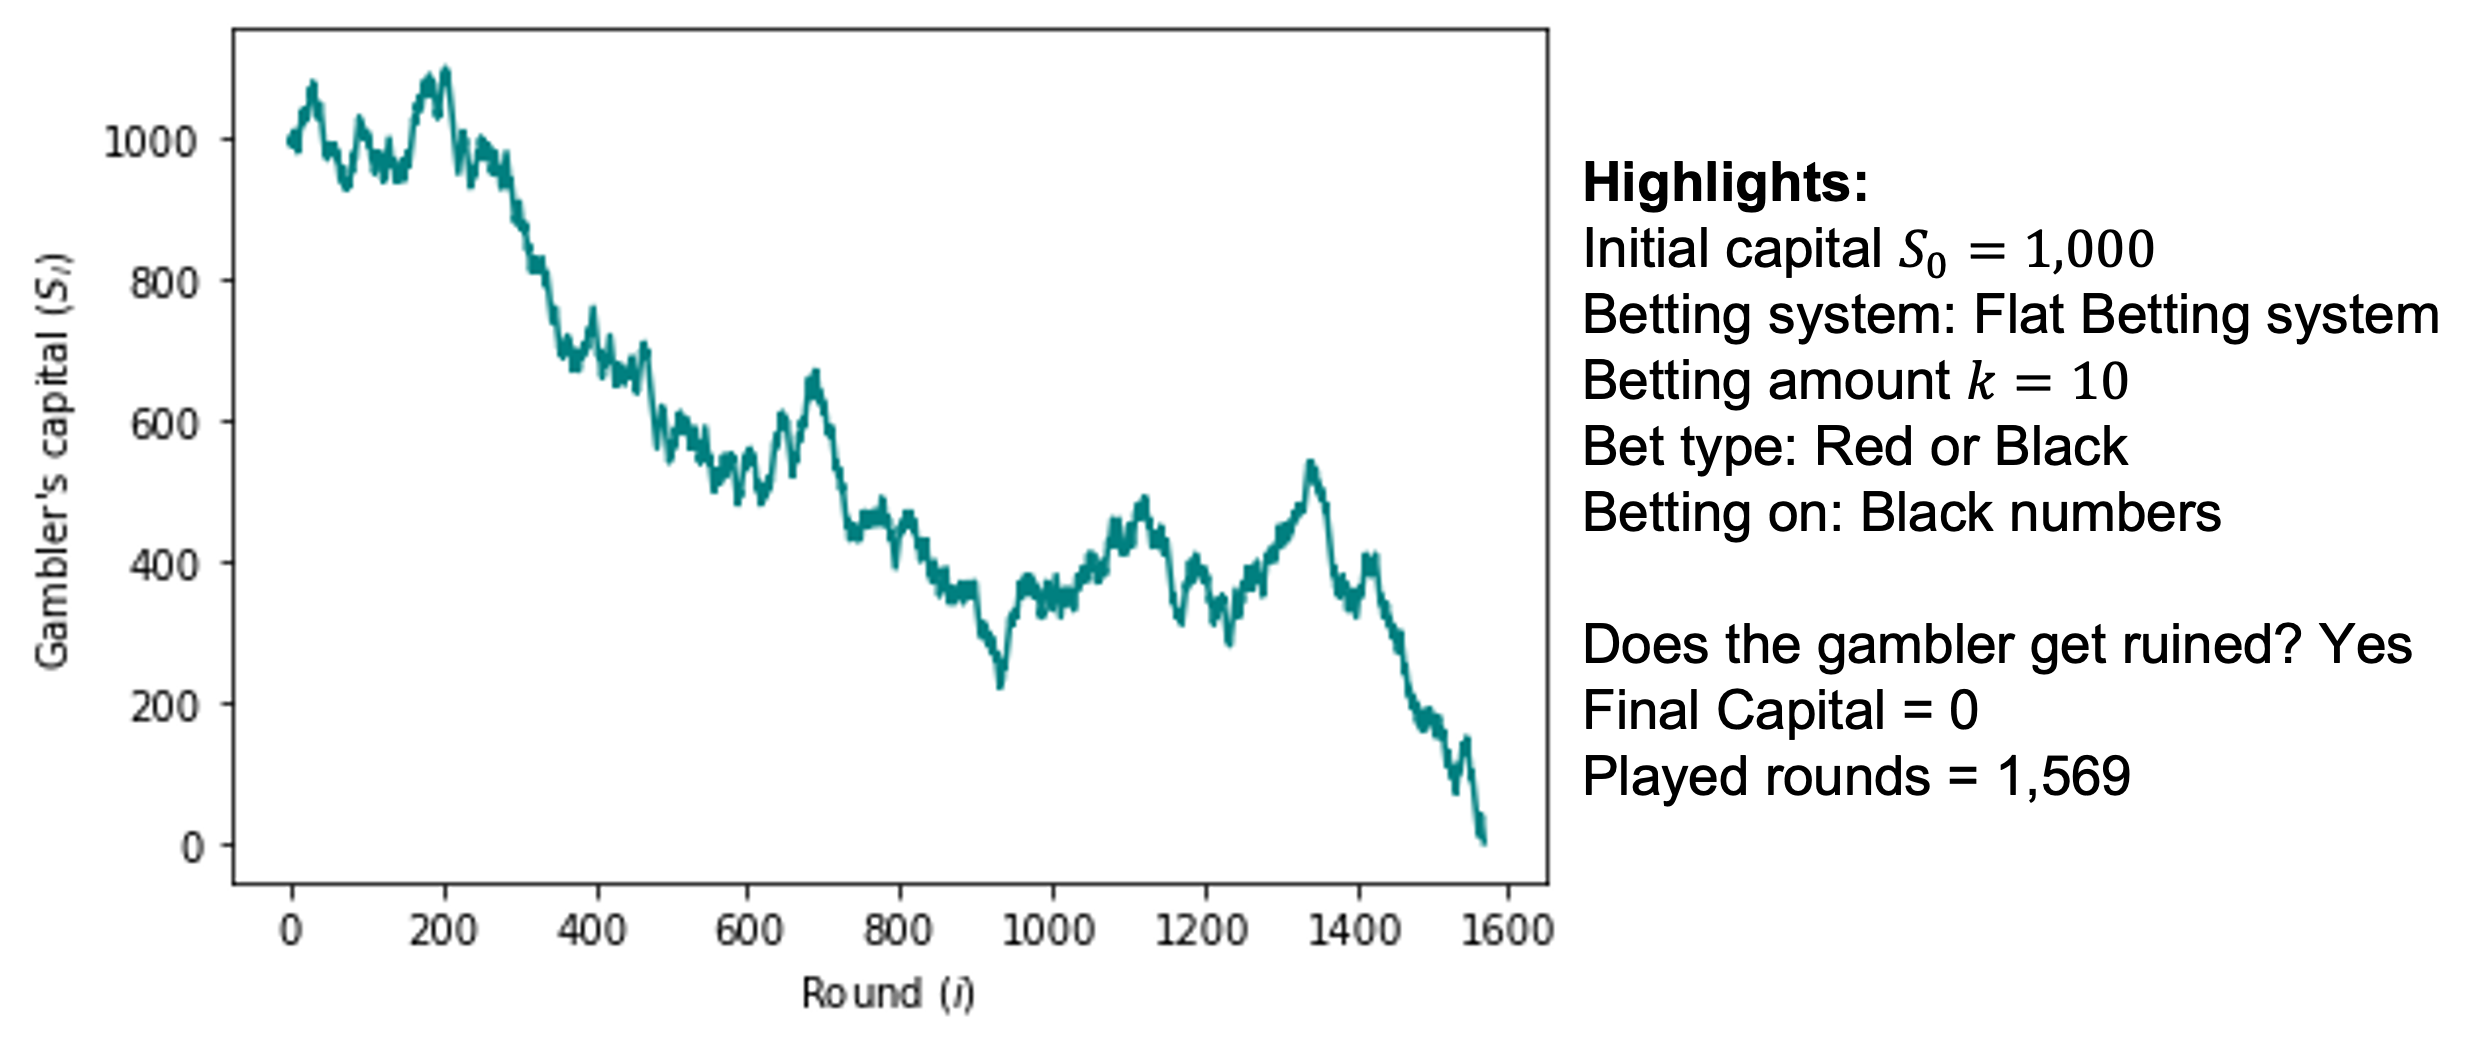
\includegraphics[width=11cm]{sim_03.png}
    \caption[Smart Live Casino - Example 3: Flat Betting System]{\textit{Smart Live Casino - Example 3: Flat Betting System}. The gambler consistently bets 10 units on the black numbers. After 1,569 rounds, the gambler faced ruin. }\label{sim_live_03}
\end{figure}

In Example 3, although the gambler eventually get ruined, the fact that the maximum value of his capital (1,100) was greater than the maximum values observed in Examples 1 and 2 (1,040 and 1,010, respectively) suggests that there were moments of success and large gains. The gambler's capital fluctuated more dramatically in Example 3 due to the higher betting amount, resulting in both larger losses and gains during the 1,569 rounds of the game.

\subsubsection{Proportional Betting System}
The proportional betting strategy is explored in Example 4. In this case, the gambler starts with an initial capital of 1000 units, consistently bets on the red numbers, and wagers 10\% of their available capital in each round. The gambler get ruined after 1,298 rounds (see Figure \ref{sim_live_p_1}).

\begin{figure}[H]
    \centering
    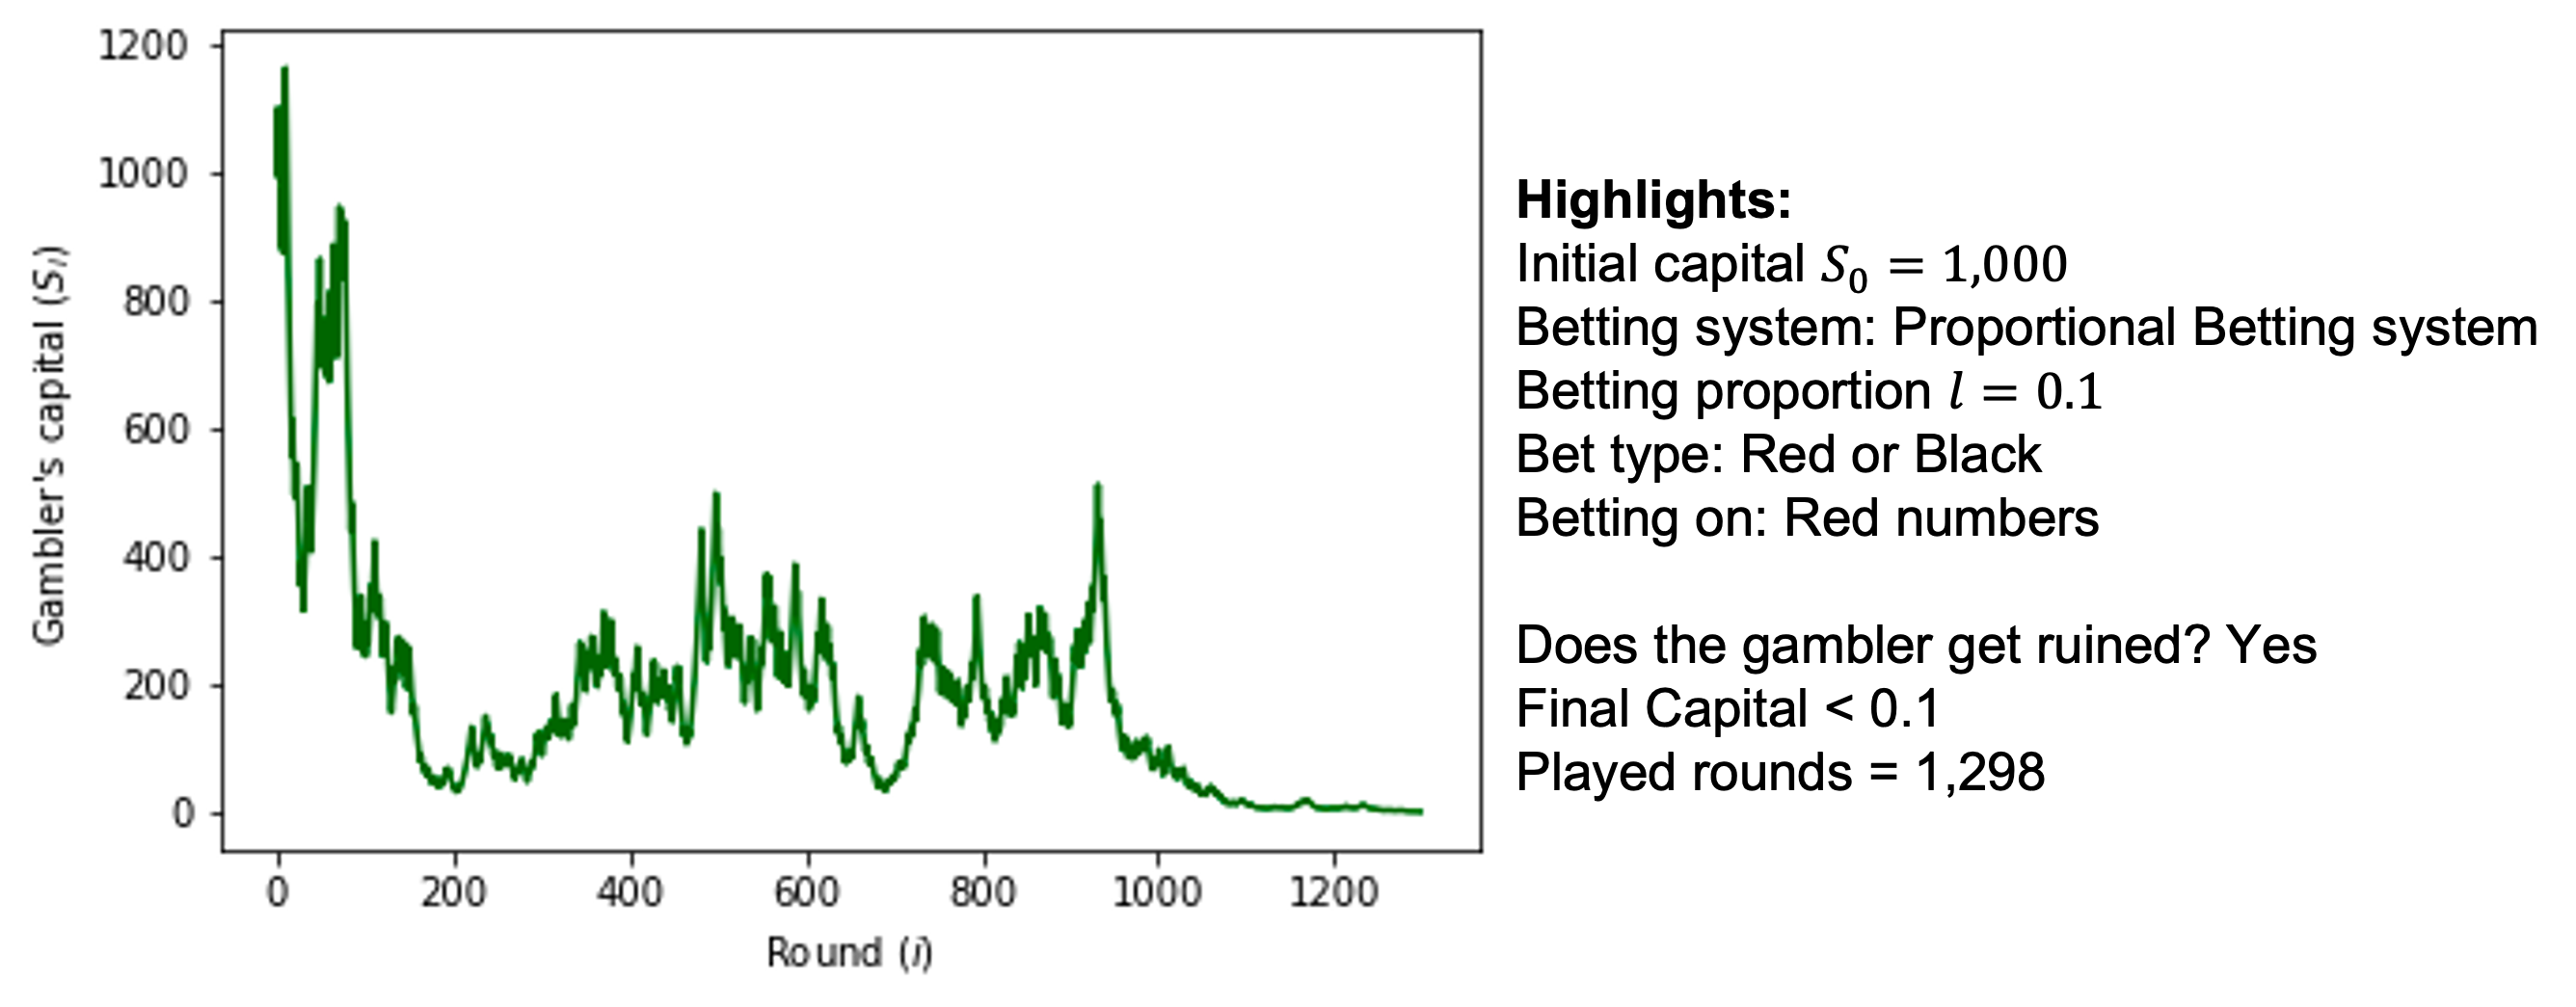
\includegraphics[width=11cm]{data_prop_1.png}
    \caption[Smart Live Casino - Example 4: Proportional Betting System]{\textit{Smart Live Casino - Example 4: Proportional Betting System.} The gambler bets 10\% of their capital in each round. Following this proportional strategy, the gambler get ruined after 1,298 rounds.}\label{sim_live_p_1}
\end{figure}

To observe the impact of the parameter $l$ on the capital path, example 5 maintains the same setup as example 4, with the exception of the value of $l$. In this scenario, the gambler bets half of their available capital in each round. Remarkably, the gambler get ruined after only 27 rounds (see Figure \ref{sim_live_p_2}), illustrating that the ruin time was significantly accelerated.

\begin{figure}[H]
    \centering
    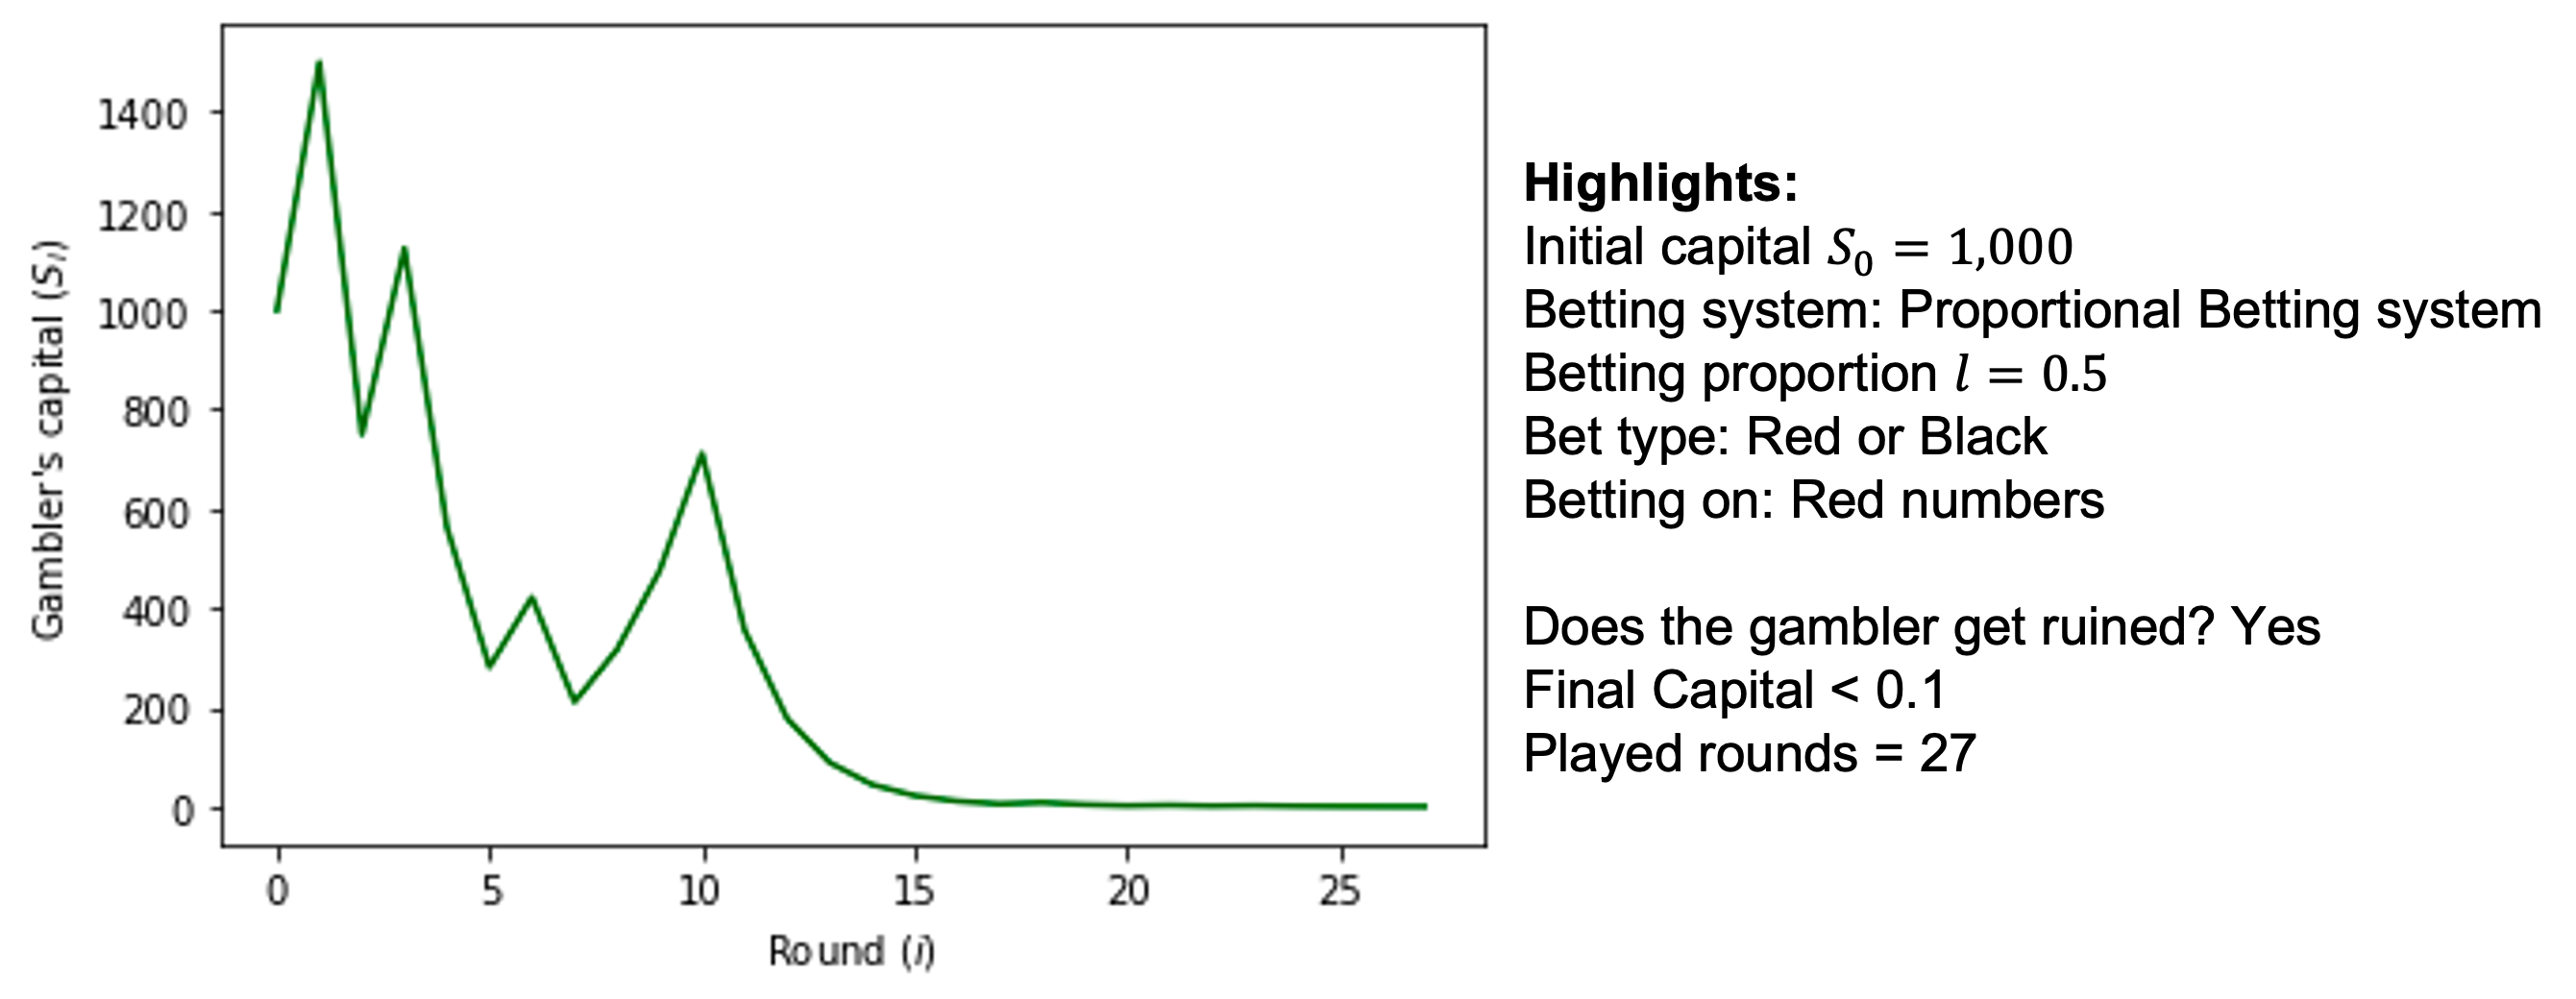
\includegraphics[width=11cm]{data_prop_2.png}
    \caption[Smart Live Casino - Example 5: Proportional Betting System]{\textit{Smart Live Casino - Example 5: Proportional Betting System.} By betting half of their available capital in each round, the gambler get ruined after only 27 rounds.}\label{sim_live_p_2}
\end{figure}
\subsubsection{Martingale Betting System}
The Martingale betting system is explored in Example 6. In this scenario, the gambler begins with an initial capital of 1000 units, starts with an initial betting amount of 1 unit, and consistently places bets on red numbers.

After 1,182 rounds, the gambler encountered a series of consecutive losses, causing their capital to decrease to 572 units. Then, the Martingale system dictated that the next bet should be 1,024 units in an attempt to recover previous losses and generate a profit. Unfortunately, the gambler was unable to sustain this strategy due to insufficient capital for placing such a substantial bet (see Figure \ref{sim_live_04}).

\begin{figure}[H]
    \centering
    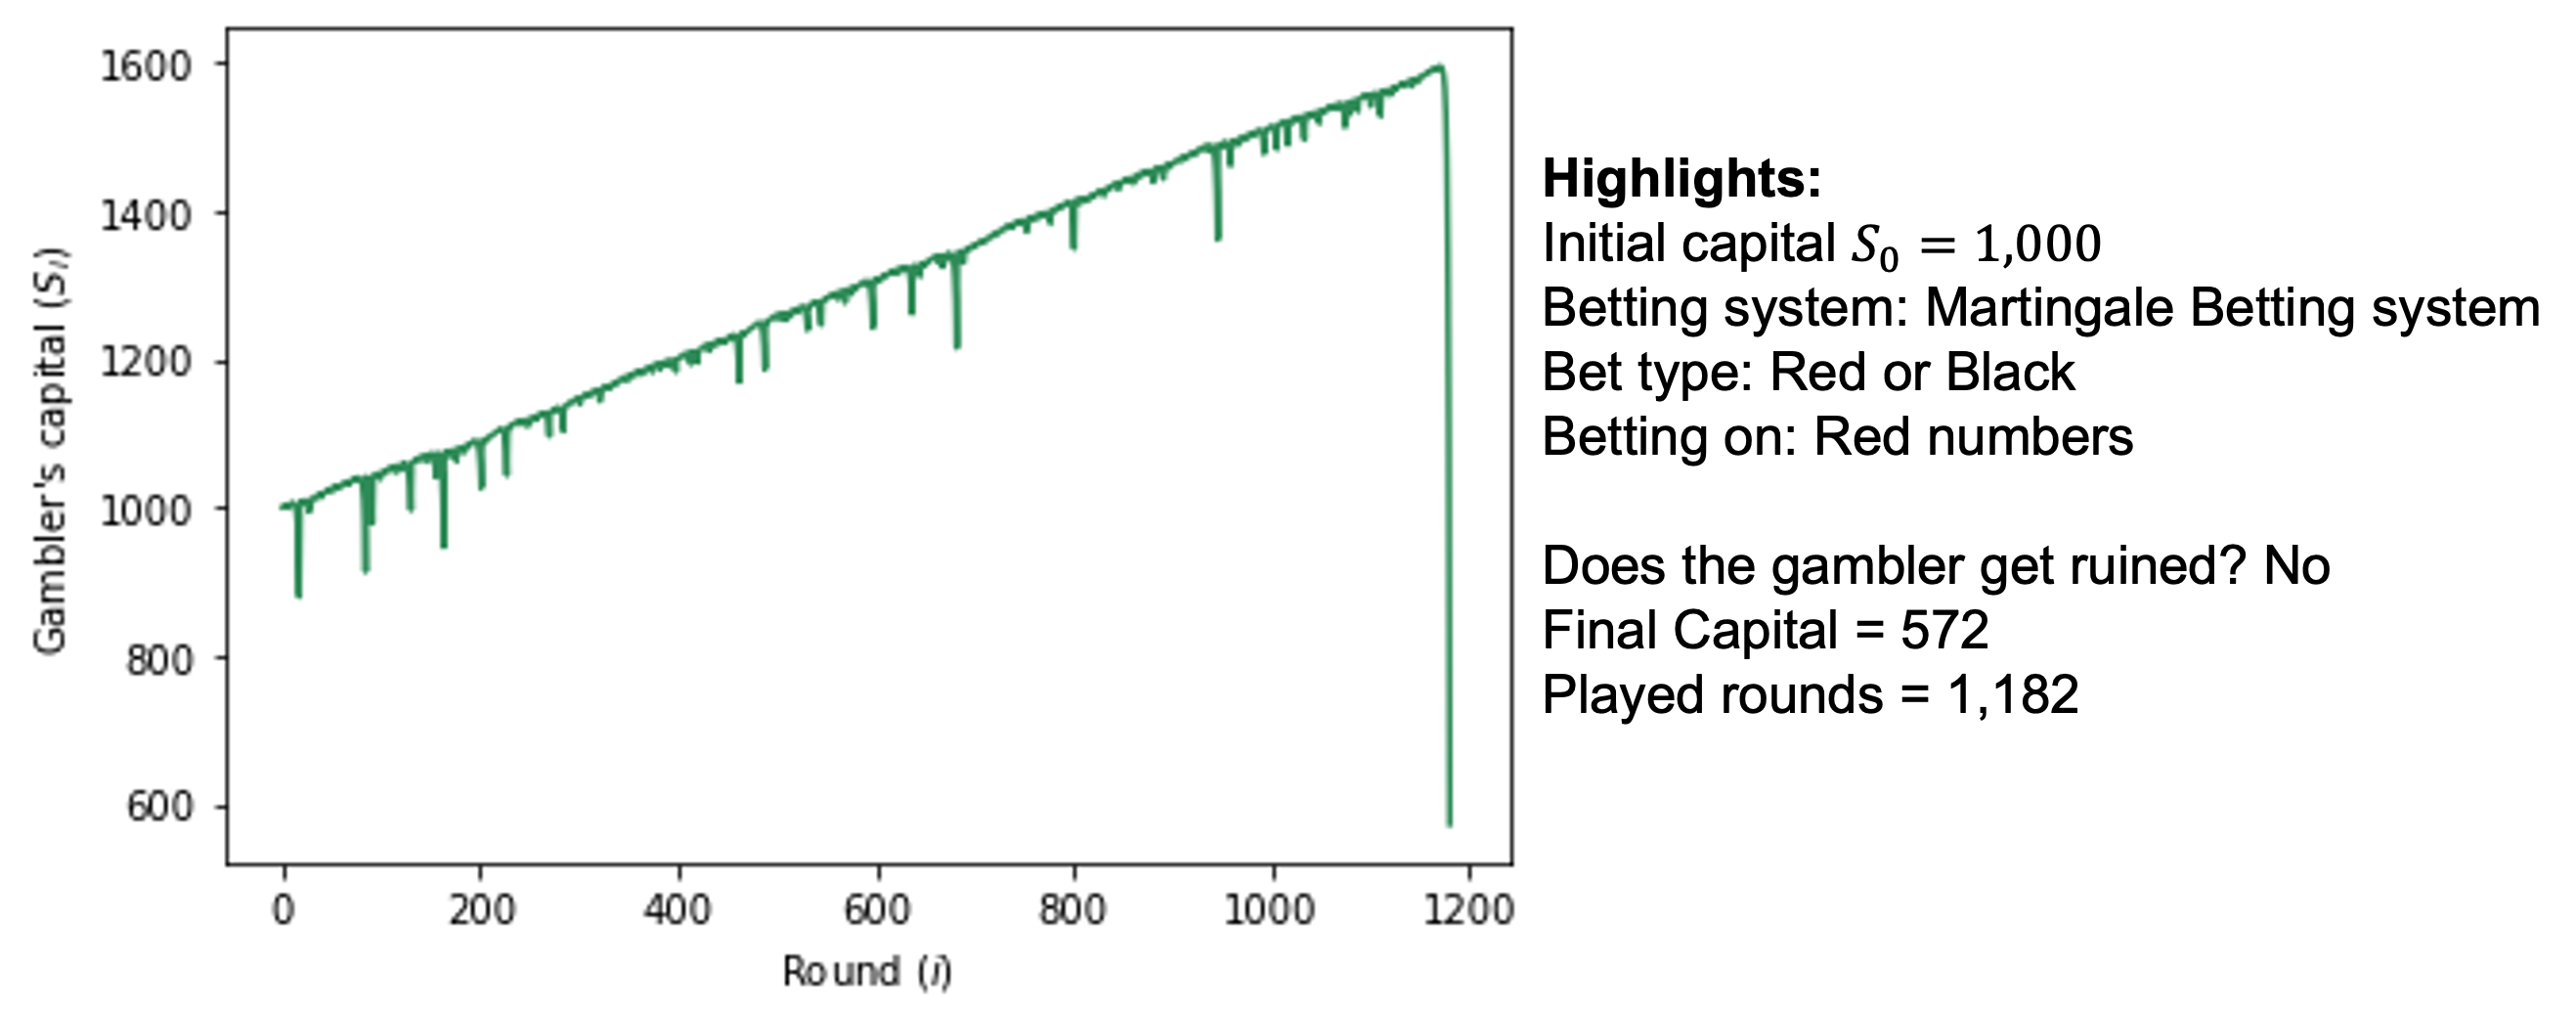
\includegraphics[width=11cm]{sim_04.png}
    \caption[Smart Live Casino - Example 6: Martingale Betting System]{\textit{Smart Live Casino - Example 6: Martingale Betting System.} The gambler stopped betting after 1,182 rounds when the strategy required a large amount to bet.}\label{sim_live_04}
\end{figure}
Before this sequence of losses, the gambler experienced some wins, accumulating a total of 1,595 in net gains. However, the Martingale system's high-risk nature became evident when the losses eventually outweighed the gains, leaving the gambler with a smaller capital than he started. In Example 6, the gambler was not ruined but was forced to stop playing due to insufficient capital to continue using the same strategy.

In Example 7, the gambler bet on a specific number (number 9) instead of the more common bet on red or black. At the start of the game, the gambler has an initial capital of $1,000$. The gambler played 774 rounds before stopping betting since the Martingale betting system required the gambler to bet $28.4$ in the next round, which exceeds the remaining capital of $22.9$. As a result, the gambler is unable to continue betting and is forced to stop playing.

\begin{figure}[H]
        \centering
        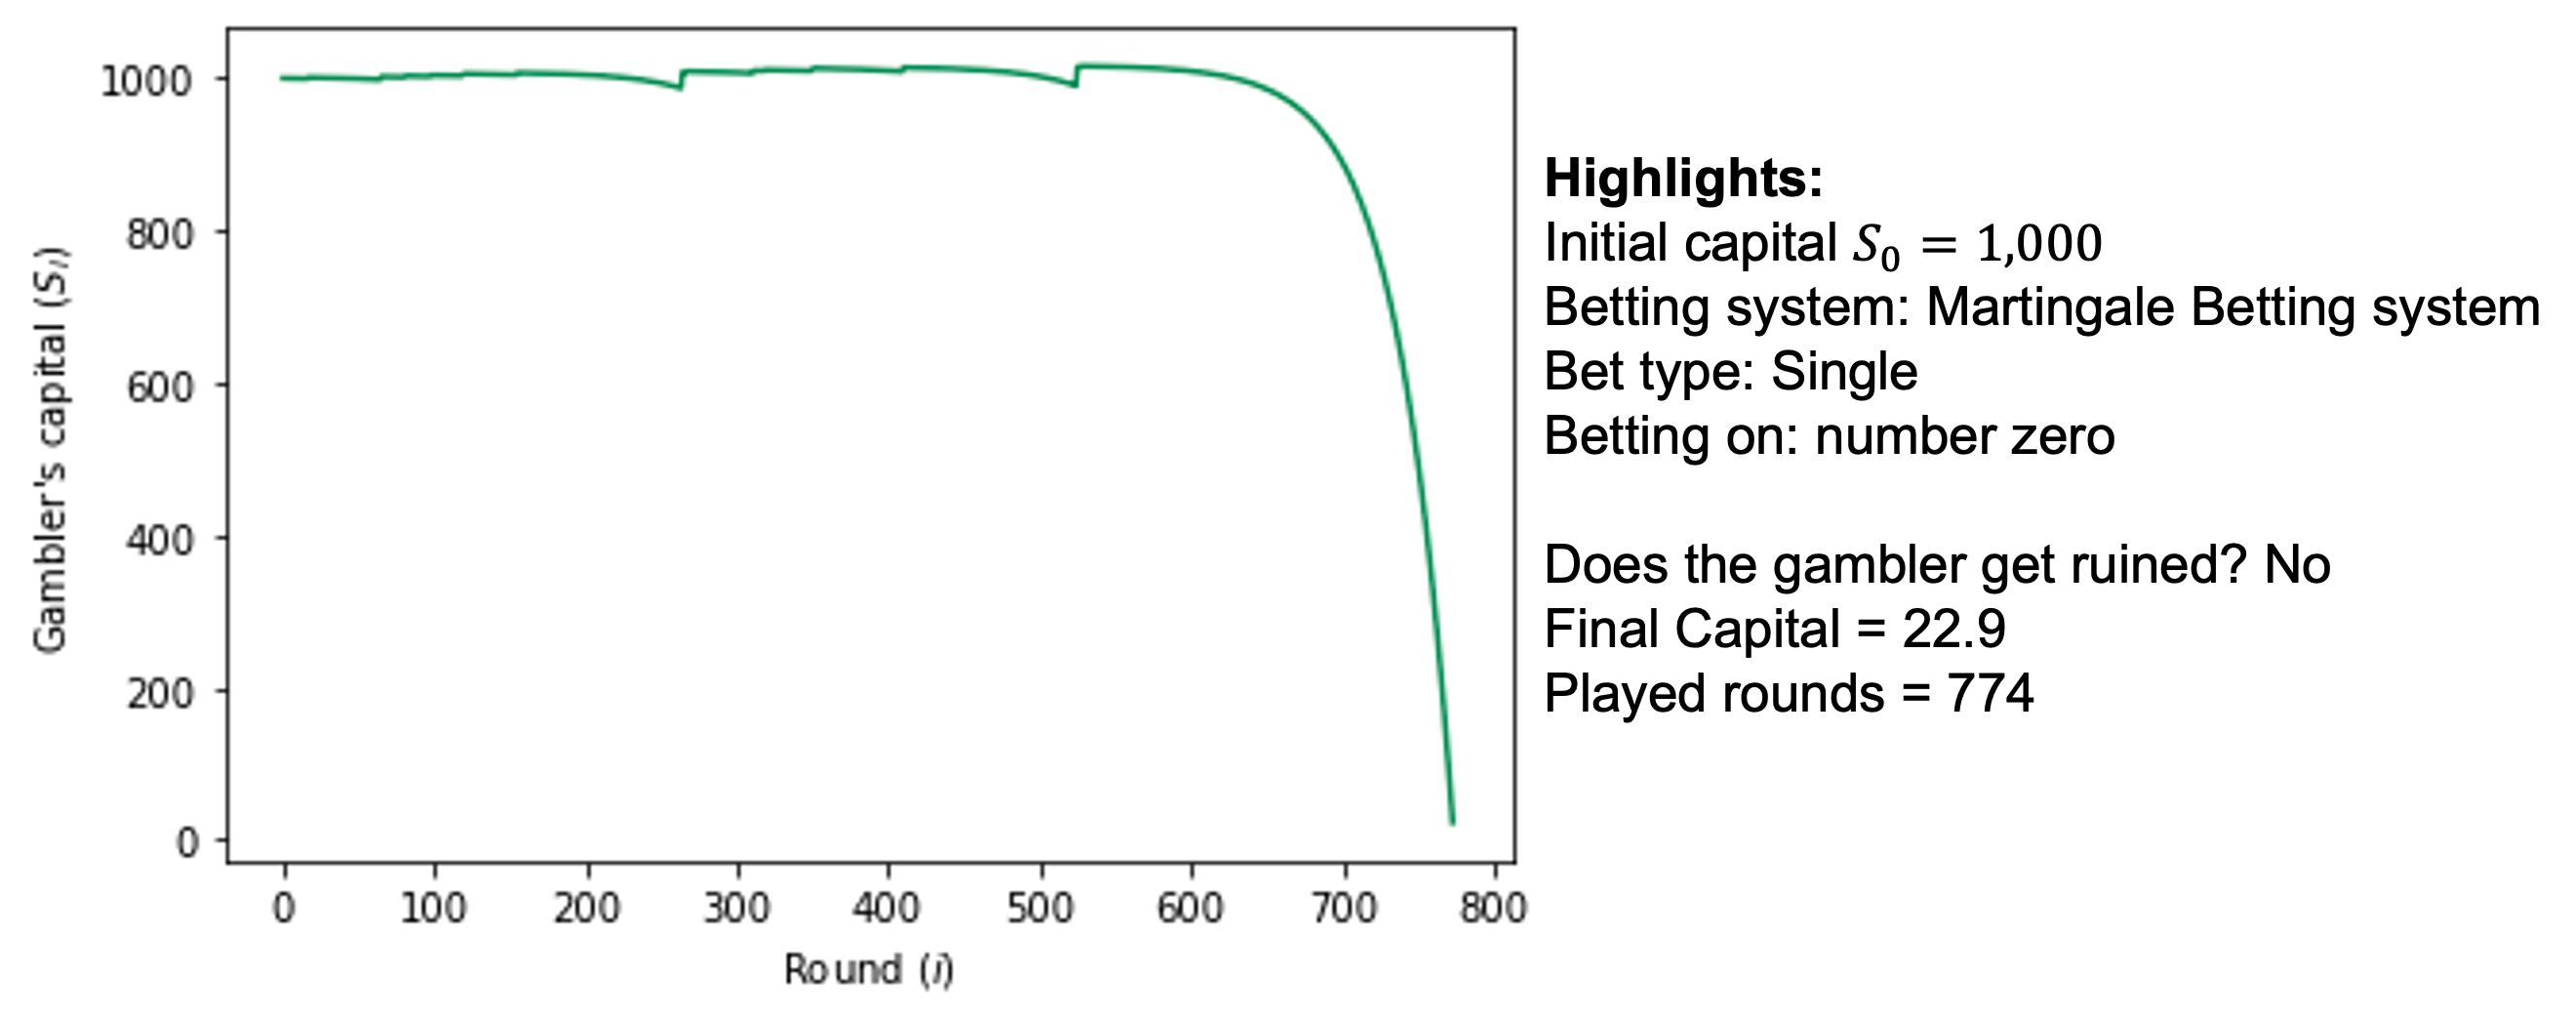
\includegraphics[width=11cm]{sim_05.png}
        \caption[Smart Live Casino - Example 7: Martingale Betting System]{\textit{Smart Live Casino - Example 7: Martingale Betting System.} When the gambler chooses a type of bet with lower probability, the number of rounds played decreases}\label{sim_live_05}
\end{figure}


Example 7 demonstrates that when a gambler chooses a type of bet with lower probability, the number of rounds played decreases, as this betting system is considered aggressive.

\subsection{Betting strategy simulation}
European roulette spins were simulated to compare the results obtained by following different betting strategies in two separate exercises. In the first exercise, the strategies compared were restricted to earning only one money unit each round, while in the second exercise, the compared strategies always bet a fixed proportion of the available capital each round. The objective of both exercises was for the gambler to achieve a profit target $G$ equal to 2, 3, ..., or 10 times the initial capital $z= 100$, that is, when target ratio equals to 1, 2, ... , 9.

For evaluating strategy performance, 10,000 simulated game scenarios were executed for each strategy. Every simulation started with an initial capital of $100$ and concluded when the player either reached their profit goal or ran out of capital to continue betting.

The assessment of betting strategy efficiency and effectiveness involved two key factors:
\begin{itemize}
    \item $P_{z,G}$: the estimated probability of achieving the goal $G$, computed using the formula:
  \begin{equation*}
      P_{z,G} = \frac{\text{Number of scenarios where gambler reaches G}}{10,000}.
  \end{equation*}
  This metric gauges the success rate of strategies in reaching the intended profit target.
  \item $D_{z,G}$: the average number of rounds taken to reach the goal $G$, calculated as:
  \begin{equation*}
      D_{z,G} = \frac{\text{Total rounds taken in scenarios where gambler reaches G}}{\text{Number of scenarios where gambler reaches G}}.
  \end{equation*}
  
This metric provides insights into the efficiency of strategies based on the time and rounds needed to attain the set goal.
\end{itemize}

Together, these metrics, $P_{z,G}$ and $D_{z,G}$, facilitate a comprehensive assessment of the strategies' performance in terms of both effectiveness and efficiency.


\subsubsection{Winning 1-unit of capital at a time}
In this exercise, the following 6 strategies winning a single monetary unit of capital in each round were compared: 

\begin{tcolorbox}[colback=gray!10,boxrule=0.25pt]
\textbf{Strategy 1}. The gambler bets consistently on a single number following the flat betting strategy with $k=1$.
\end{tcolorbox}

\begin{tcolorbox}[colback=gray!10,boxrule=0.25pt]
\textbf{Strategy 2}. The gambler bets consistently on one of the 3 dozens following the flat betting strategy with $k=1$.
\end{tcolorbox}

\begin{tcolorbox}[colback=gray!10,boxrule=0.25pt]
\textbf{Strategy 3}. The gambler bets consistently on one color black or red following the flat betting strategy with $k=1$.
\end{tcolorbox}

\begin{tcolorbox}[colback=gray!10,boxrule=0.25pt]
\textbf{Strategy 4}. The gambler bets consistently on a single number following the martingale betting strategy.
\end{tcolorbox}

\begin{tcolorbox}[colback=gray!10,boxrule=0.25pt]
\textbf{Strategy 5}. The gambler bets consistently on one of the 3 dozens following the martingale betting strategy.
\end{tcolorbox}

\begin{tcolorbox}[colback=gray!10,boxrule=0.25pt]
\textbf{Strategy 6}. The gambler bets consistently on one color black or red following the martingale betting strategy.
\end{tcolorbox}

The primary goal of this exercise is to investigate strategies designed to achieve a specific winning outcome—a single monetary unit—in each round. The selection of these 6 strategies followed 2 reasons. First, the omission of the proportional betting system from this exercise is a deliberate choice because, unlike the flat and martingale strategies, which aim to win a fixed amount of money in each round, the proportional betting system operates on a different principle (adjusting the bet size based on the current capital). Second, the inclusion of three types of flat betting and three types of Martingale systems was strategically motivated by gambler's different risk appetite. Each of these bet types was deliberately classified as low, medium, or high risk, reflecting distinct risk tolerance levels. This approach allowed us to account for a spectrum of gambler preferences, from those who prefer cautious, low-risk strategies to those seeking potentially higher rewards despite increased risk.

The above-mentioned strategies were evaluated across different target ratios (1 to 9), representing the desired profit relative to the initial capital ($z=100$). Table \ref{results_exercise1_1} and \ref{results_exercise1_2} present the estimated $P_{z,G}$ and $D_{z,G}$, respectively. 

\begin{table}[h!]
\centering
\caption{Probability of reaching the goal - Winning 1-unit of capital at a time exercise}
\begin{tabular}{|c|c|c|c|c|c|c|}
\hline
Target ratio & Strategy 1 &  Strategy 2 &  Strategy 3 &  Strategy 4 & Strategy 5 &  Strategy 6 \\
$G/S_{0}$ &  &  &  &   &  &  \\
\hline\hline
1 &0.356&0.369&0.366& 0.463&0.392&0.331\\
2 &0.171&0.170&0.179&0.290&0.212&0.163\\
3 &0.091&0.090&0.089&0.205&0.149&0.112\\
4 &0.052&0.051&0.054&0.168&0.104&0.078\\
5 &0.028&0.030&0.026&0.138&0.085&0.051\\
6 &0.015&0.016&0.016&0.111&0.064&0.039\\
7 &0.010&0.010&0.009&0.099&0.061&0.036\\
8 &0.005&0.005&0.006&0.089&0.047&0.029\\
9 &0.002&0.003&0.004&0.075&0.040&0.024\\
\hline
\end{tabular}
\label{results_exercise1_1}
\end{table}

Observing Table \ref{results_exercise1_1}, we can see that Strategy 4 demonstrates the highest probability of reaching the profit goal across all target ratios. On the other hand, Strategy 6 shows the lowest probability of reaching the goal. Additionally, the flat betting strategies (Strategies 1 to 3) generally exhibit lower probabilities of reaching the target compared to the martingale strategies.

\begin{table}[h!]
\centering
\caption{Average number of rounds until reaching the goal-  Winning 1-unit of capital at a time exercise}
\begin{tabular}{|c|c|c|c|c|c|c|}
\hline
Target ratio & Strategy 1 &  Strategy 2 &  Strategy 3 &  Strategy 4 & Strategy 5 &  Strategy 6 \\
$G/S_{0}$ &  &  &  &   &  &  \\
\hline\hline
1 &35,669&1,990&979&2,454&179&107\\
2 &61,427&3,496&1,742&3,865&263&155\\
3 &82,679&4,734&2,293&4,704&319&182\\
4 &99,357&5,579&2,804&5,419&356&201\\
5 &107,206&6,135&2,985&5,987&388&215\\
6 &114,867&6,406&3,210&6,366&405&224\\
7 &120,115&6,627&3,387&6,873&437&235\\
8 &123,461&6,967&3,530&7,223&446&238\\
9 &123,161&7,177&3,627&7,524&459&240\\
\hline
\end{tabular}
\label{results_exercise1_2}
\end{table}

Analyzing Table \ref{results_exercise1_2}, we find that the average number of rounds required to achieve the profit goal is generally higher for all strategies when the target ratio increases. Strategy 4 still stands out as the most efficient strategy in achieving the profit goal with the lowest average number of rounds across all target ratios. Conversely, Strategy 6 consistently requires the highest number of rounds on average.

In this exercise, Martingale strategies demonstrated the highest probability of reaching the profit goal across all target ratios. However, this strategy's heavy reliance on capital availability could lead to unsustainable bets and eventual failure. Conversely, strategies that involved flat betting, whether on a single number, a dozen, or a color, exhibited similar success rates. While these strategies provided consistent bet sizes, their probabilities of achieving the profit goal were generally lower compared to the Martingale strategy.

The recommendation for a gambler who aims to win 1 unit at a time in order to reach a total target of $G$ is as follows: If their priority is to maximize the probability of reaching the goal, then employing the Martingale system while betting on any bet type with a large payoff may be the most suitable choice. However, if the gambler also intends to minimize the average time required to reach the goal, then employing the Martingale system while considering the lowest-risk bet might be the correct choice.

\subsubsection{Fixed proportion of capital bet at a time}
In this exercise, the 4 compared strategies always bet a fixed proportion $l$ of the available capital each round. For each combination of target ratio from 1 to 9, and betting proportion $l$ ranging from $0.1$ to $1$, 10,000 scenarios were generated for the following strategies:

\begin{tcolorbox}[colback=gray!10,boxrule=0.25pt]
\textbf{Low-Risk Strategy}: The gambler consistently bets on the red numbers following a proportional betting strategy.
\end{tcolorbox}

\begin{tcolorbox}[colback=gray!10,boxrule=0.25pt]
\textbf{Medium-Risk Strategy}: The gambler consistently bets on one of the three dozens following a proportional betting strategy.
\end{tcolorbox}

\begin{tcolorbox}[colback=gray!10,boxrule=0.25pt]
\textbf{High-Risk Strategy}: The gambler consistently bets on a single number following a proportional betting strategy.
\end{tcolorbox}

\begin{tcolorbox}[colback=gray!10,boxrule=0.25pt]
\textbf{Mixed-Risk Strategy}: The gambler consistently bets $lS_{i}$ as follows:
\begin{itemize}
    \item On a single number if $S_{i} < 0.3 G$ (High-risk bet)
    \item On a dozen if $0.3 G \leq S_{i} < 0.7 G$ (Medium-risk bet)
    \item On black/red numbers if $0.7 G \leq S_{i}$ (Low-risk bet)
\end{itemize}
\end{tcolorbox}

The motivation for this exercise is to analyze and compare two distinct approaches to gambling risk management: single-type risk strategies and mixed risk strategies. The risk level associated with each strategy in this exercise is determined by the probability outcome of the bets rather than the bet amounts. The categorization of “low”, “medium”, and “high” risk is based on the inherent probabilities of winning for each type of bet. Despite each strategy following the same rule for determining the bet amount (a fixed proportion of the available capital), their riskiness is dictated by the probability of winning associated with the specific type of bet they consistently employ.



Figures \ref{graf:proba} and \ref{graf:round} presents the simulated ruin probability and the average number of rounds until reaching the goal for the fixed proportion of capital bet at a time exercise.
Figure \ref{graf:proba} depicts the change in the estimated probability $P_{z,G}$ of reaching the profit goal for different strategies and target ratios. The consistent trend observed is that as the target ratio increases (indicating a higher profit goal relative to the initial capital), the probability of achieving that goal decreases. This holds true for all strategies, regardless of the chosen bet proportion $l$. Notably, the mixed risk strategy demonstrates a slight advantage over the high risk strategy in terms of reaching the profit goal, especially when the chosen $l$ is smaller. This difference becomes more pronounced as $l$ decreases.

\begin{figure}[H]
        \centering
        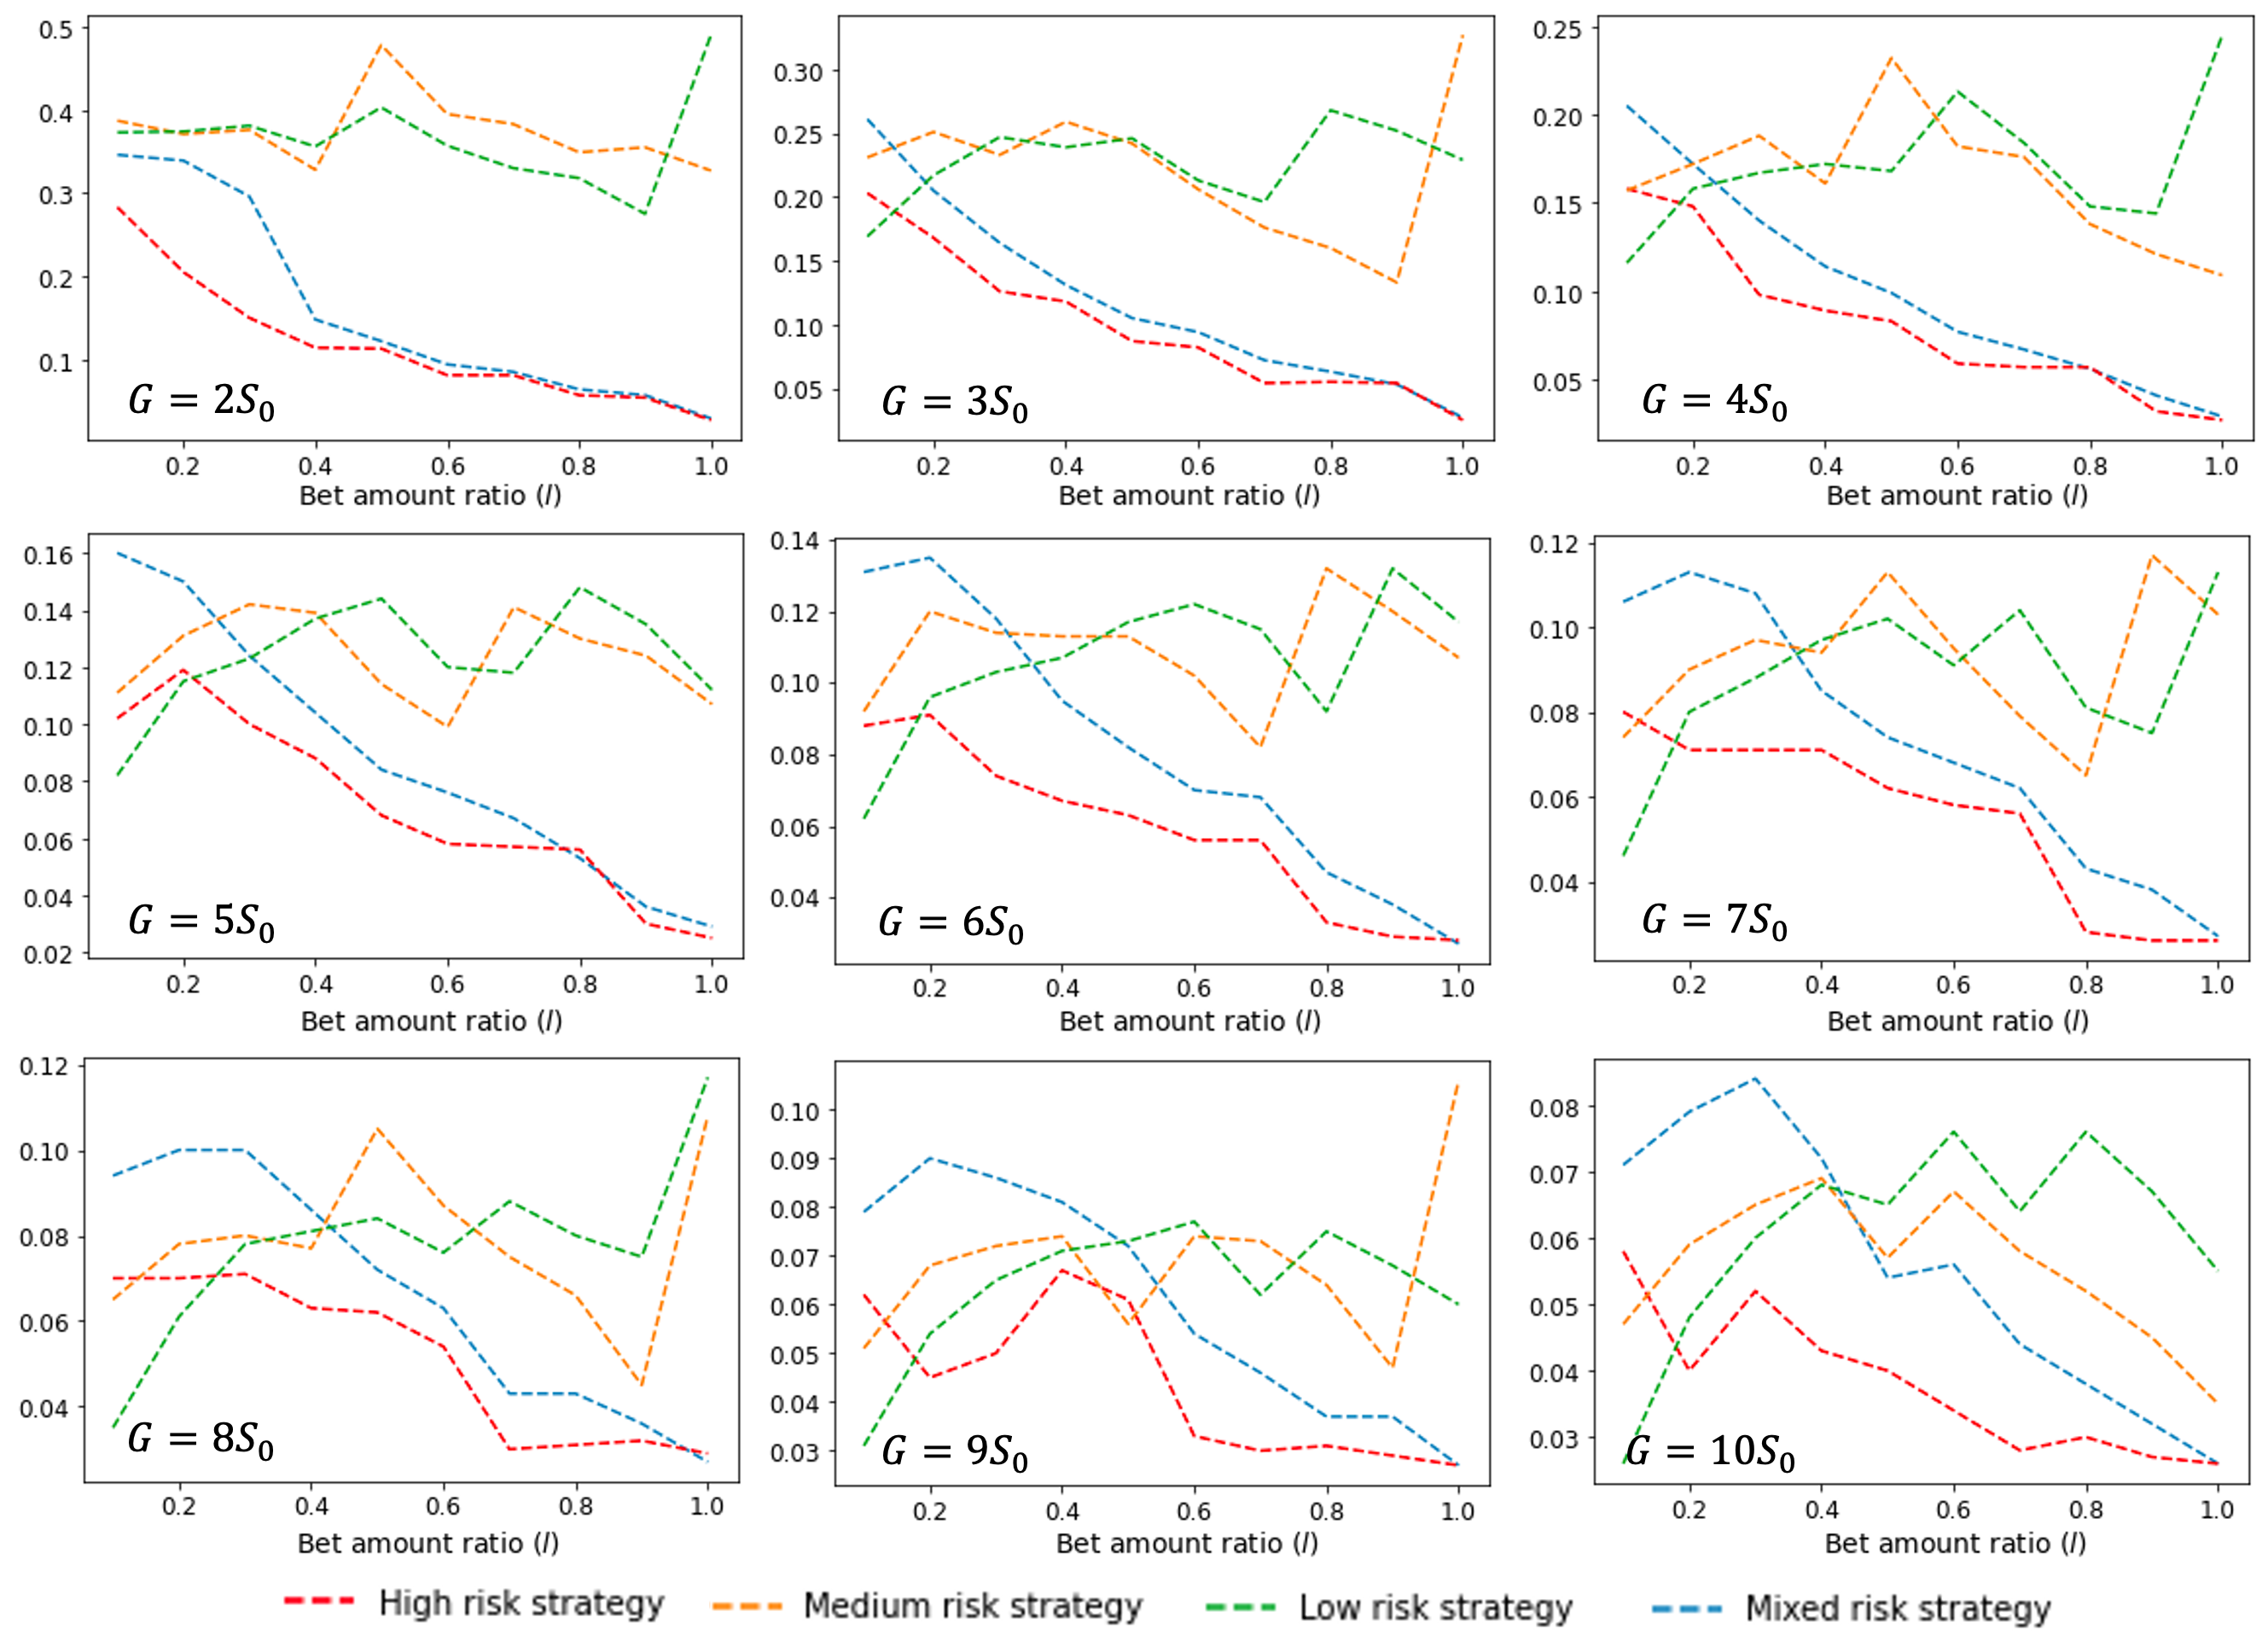
\includegraphics[width=15cm]{proba_results.png}
        \caption[Fixed proportion of capital bet at a time exercise -  Probability of reaching G]{\textit{Estimated probability of reaching G}. Probability $P_{z,G}$ consistently decreases as the target ratio increases for all the strategies, regardless of the chosen bet proportion $l$. The mixed risk strategy showcases a marginal out-performance compared to the high risk strategy, with this difference becoming more pronounced as $l$ decreases. }\label{graf:proba}
\end{figure}
\begin{figure}[H]
        \centering
        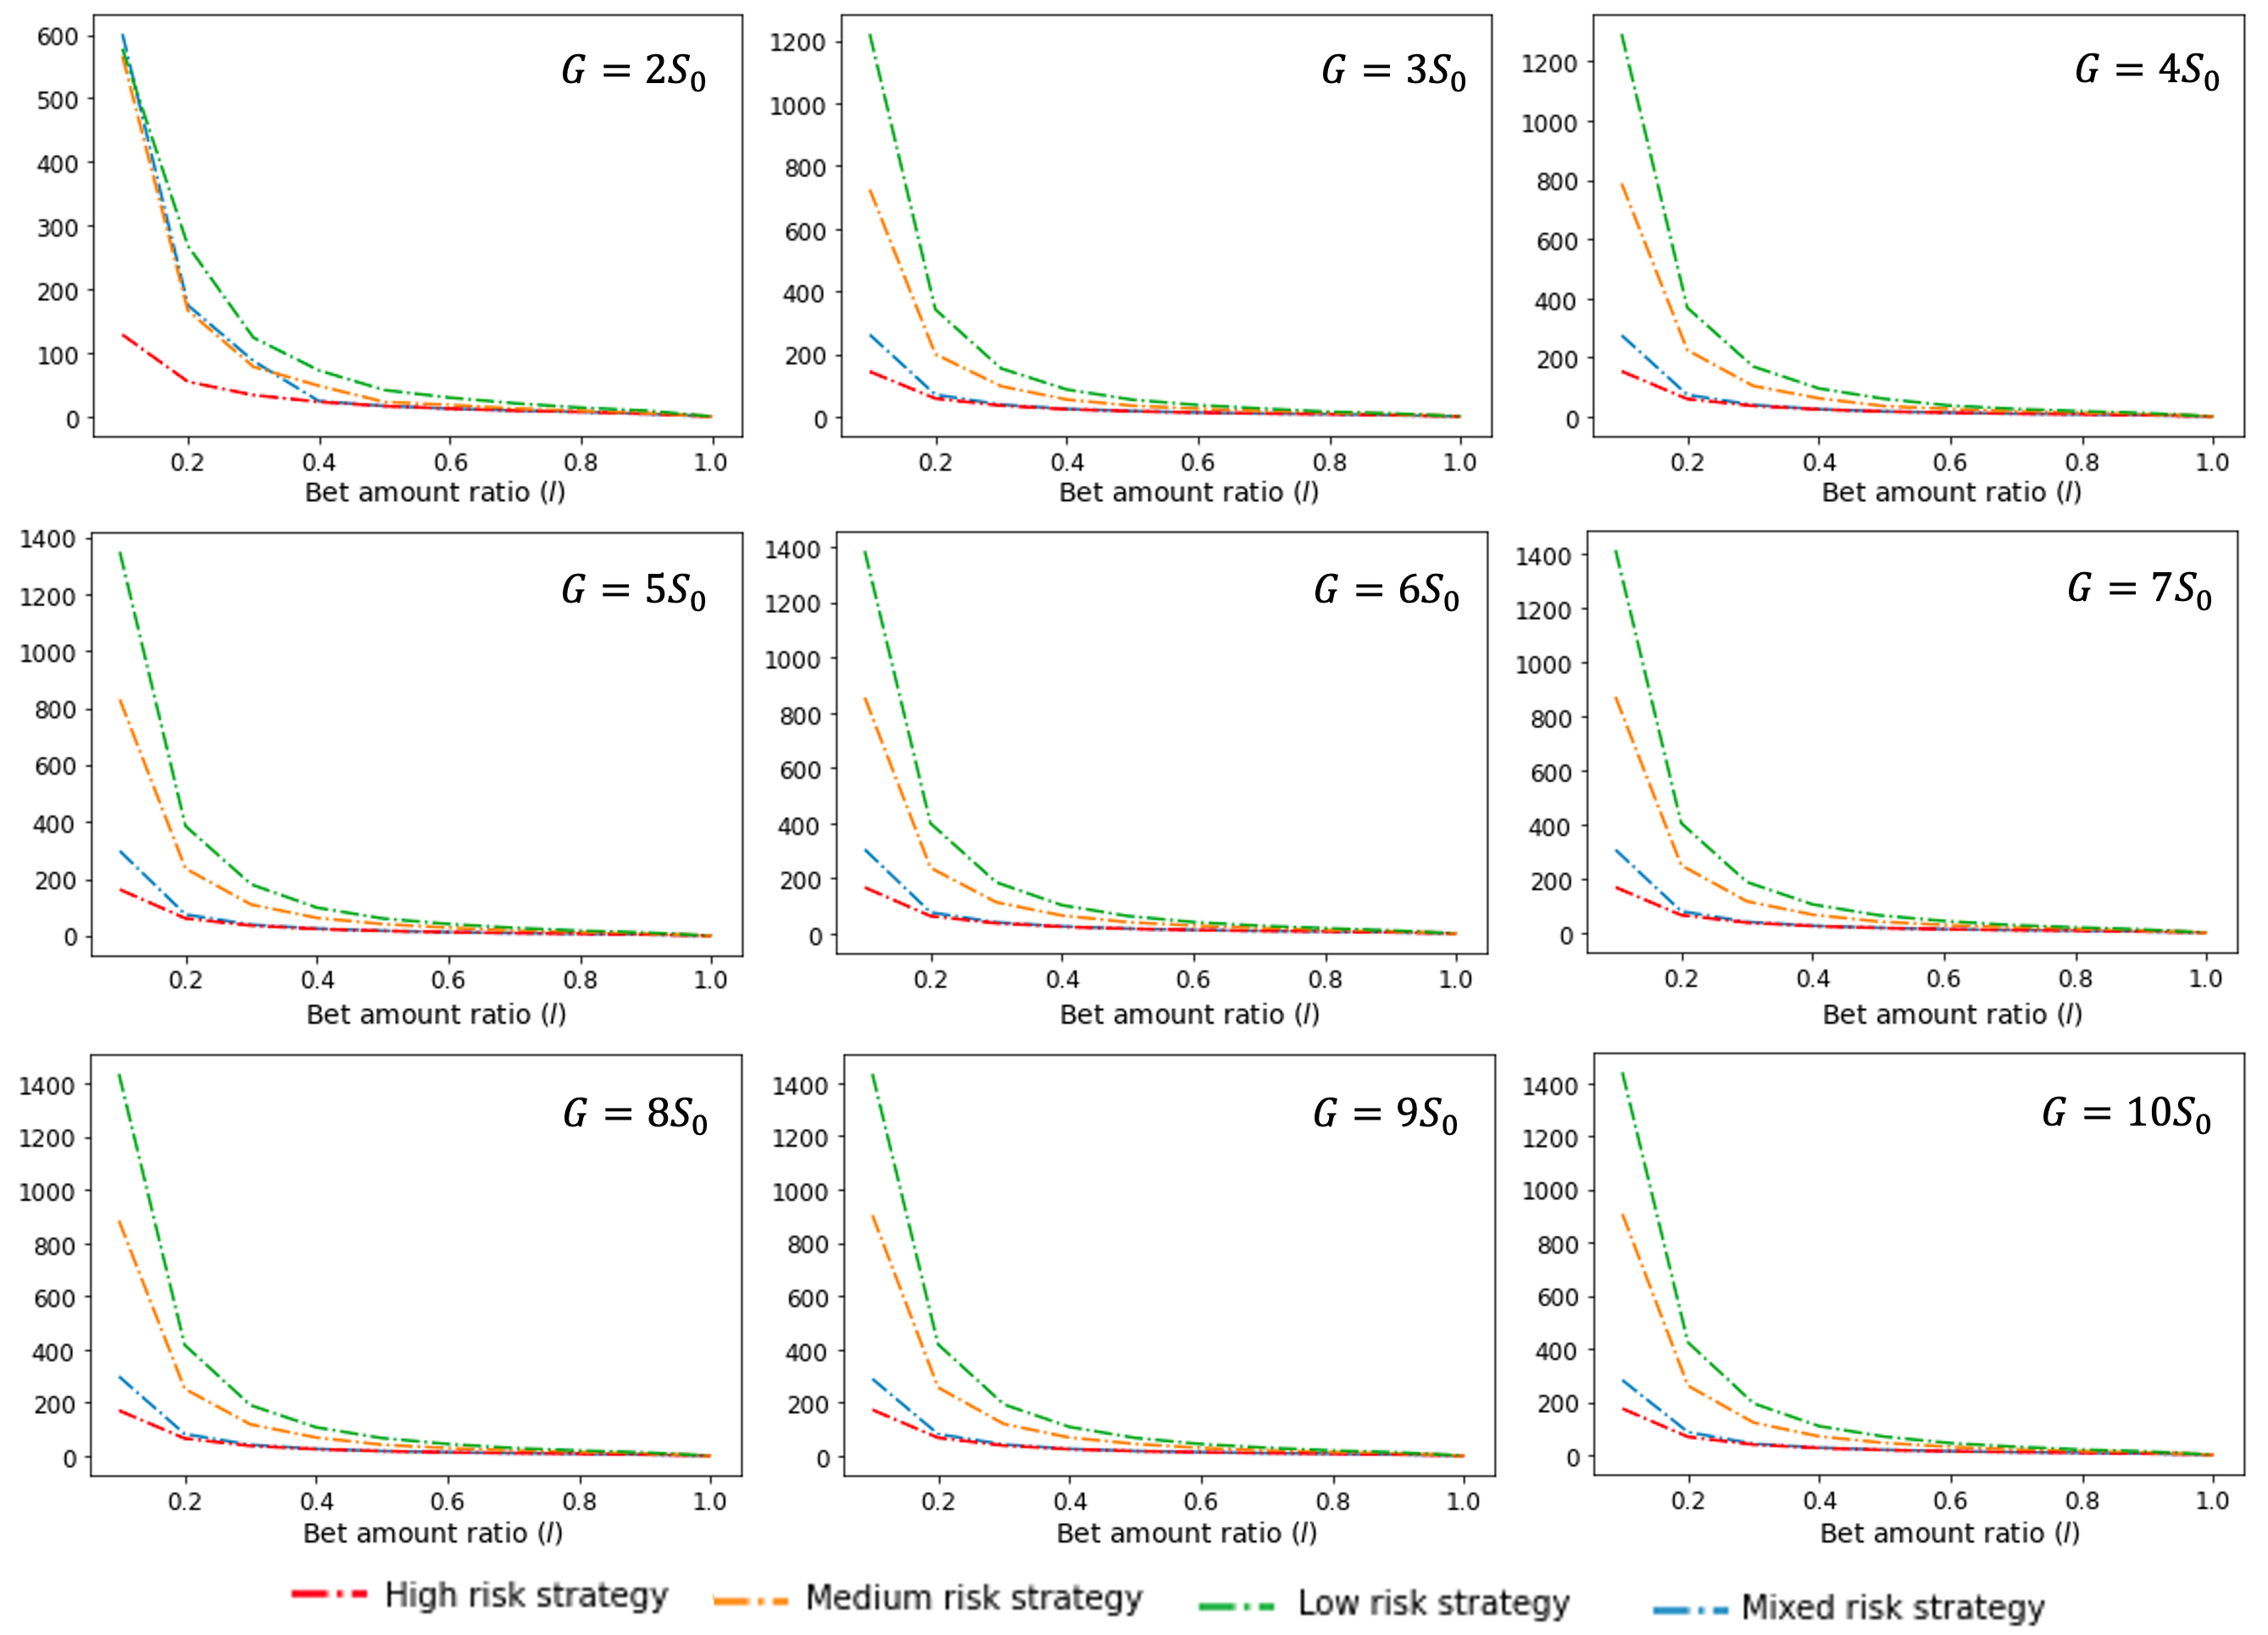
\includegraphics[width=15cm]{results_rounds.png}
        \caption[Fixed proportion of capital bet at a time exercise - Number of rounds until reaching G]{\textit{Estimated number of rounds until reaching G}. there is an inverse relation between the risk level and the avergae number of rounds. The behavoiur of the $D_{z,G}$ if consintent along the different goals $G$. }\label{graf:round}
\end{figure}

In Figure \ref{graf:round}, the inverse relationship between risk level and the average number of rounds until reaching the profit goal ($D_{z,G}$) is highlighted. As the risk level increases (from low to high risk strategies), the average number of rounds needed to achieve the goal decreases. This behavior remains consistent across different target ratios ($G$), indicating that higher risk strategies tend to achieve the goal in fewer rounds. This aligns with the concept that riskier strategies have the potential for faster capital growth but also higher volatility.

The following function were used to combine both the probability of reaching the goal and the average number of rounds until reaching the goal:

\begin{equation}
    f(l, G_z) = \frac{D_{z,G}}{P_{z,G}^{2}}.
\end{equation}

The rationale behind using this function is to identify strategies that strike a balance between two key factors. The function yields smaller values for strategies that achieve a delicate equilibrium between efficient and effective performance. Essentially, the function values strategies that not only offer higher odds of reaching the goal but also do so with fewer rounds. This translates to strategies that manage to minimize \(D_{z,G}\) (requiring fewer rounds) while simultaneously maximizing \(P_{z,G}\) (having a higher likelihood of reaching the goal). In simpler words, the focus is on strategies that efficiently attain the objective while ensuring a strong chance of success.

Figure \ref{graf:function} depicts this function $f(l, G_z)$ behavior. In general, the mixed risk strategy shares similarities with the high risk strategy. However, the behavior shifts when the goal is to double the initial capital. In this specific scenario, the mixed risk strategy deviates from the high risk strategy and aligns more closely with the low and medium risk strategies.
\begin{figure}[H]
        \centering
        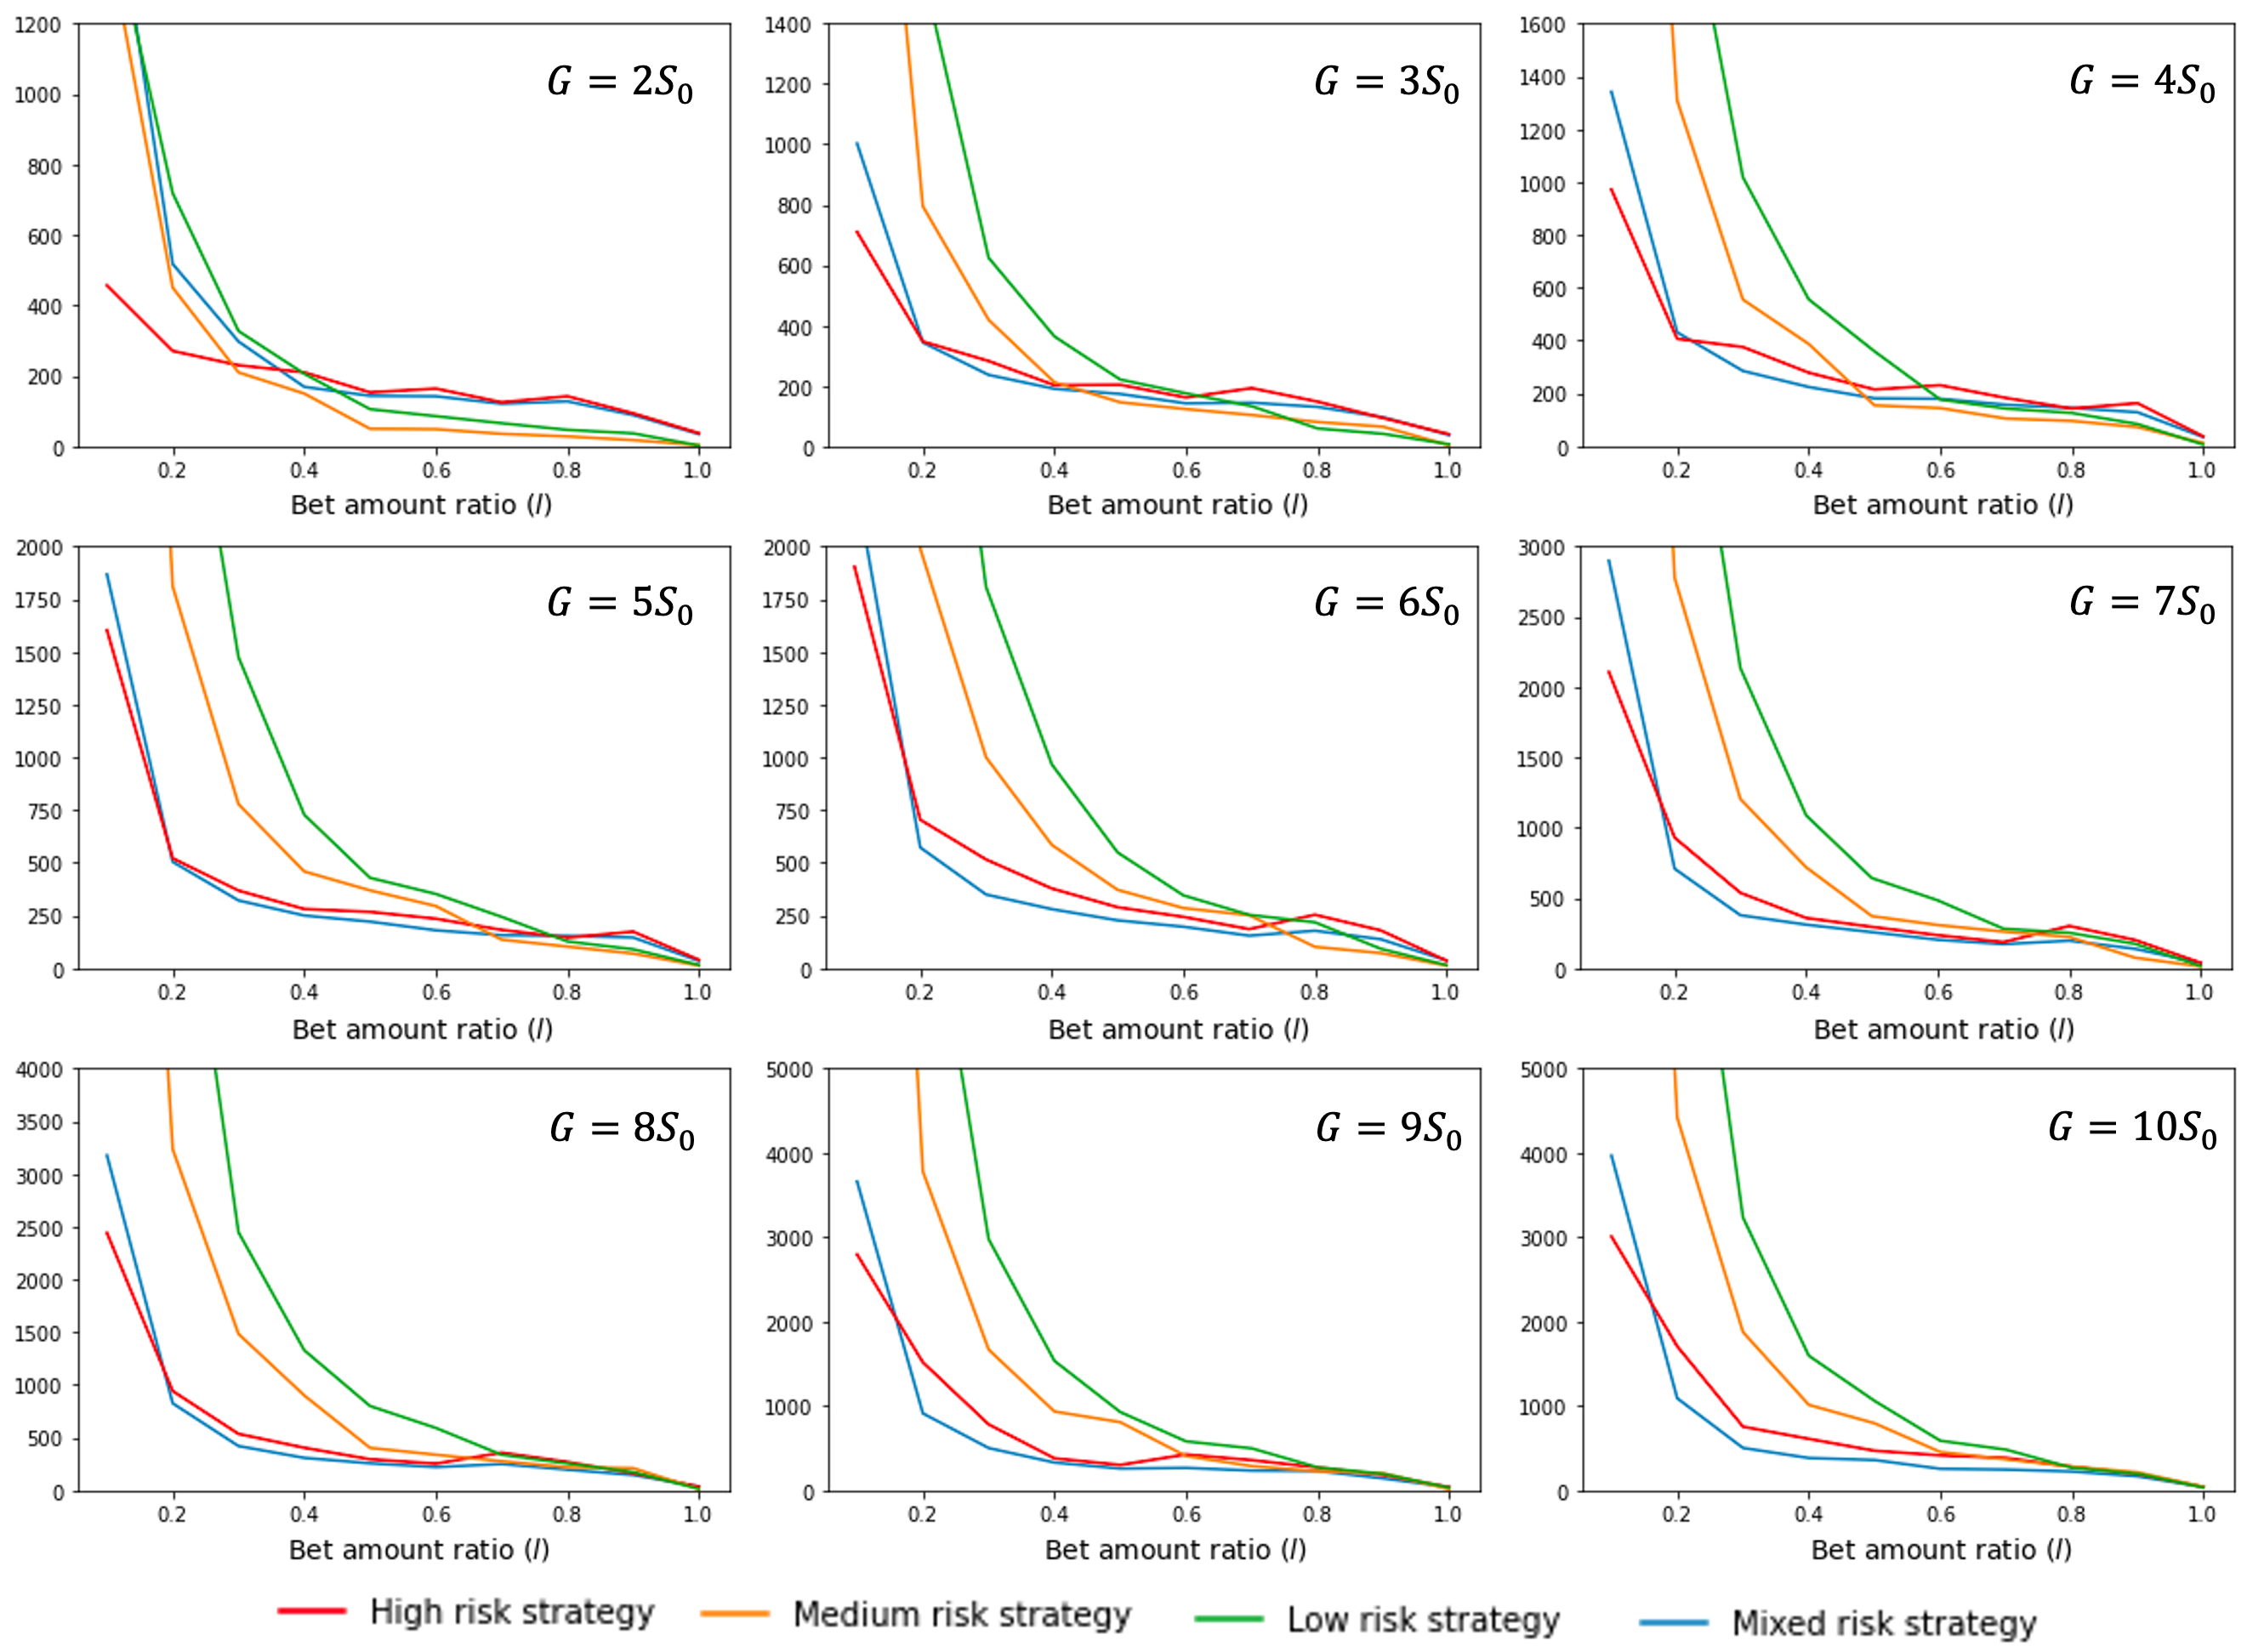
\includegraphics[width=16cm]{result_f.png}
        \caption[Combination of the $P_{z,G}$ and $D_{z,G}$]{\textit{Combination of the $P_{z,G}$ and $D_{z,G}$}.  The mixed risk strategy behaves like the high risk strategy offering low number or rounds. Except when the goal is doubling the initial capital in that case, the mixed risk strategy behaves like the low and medium risk strategies.}\label{graf:function}
\end{figure}

The empirical analysis reveals that the risk adaptable strategy exhibits performance characteristics similar to a high-risk strategy. As a result, this strategy can be recommended for individuals who have a preference for high-risk bets and a fixed target. This strategy aligns with the high-risk approach during its initial phase, offering the potential for significant capital growth through riskier bets. It's well-suited for those who are comfortable with the inherent volatility and uncertainty associated with high-risk gambling.

Finally, consider Figure \ref{graf:final_graph}, which illustrates a comparative scenario featuring four players  placing bets simultaneously. Each player employs a distinct strategy: low risk, medium risk, high risk, and a mixed risk strategy. For this illustration, we assume that each player starts with an initial capital of 10 and aims to achieve a profit target of 100. The bet amount proportion, $l$, is fixed at 0.05.

Over the course of the initial 70 rounds, players who adopt either the risk-adapted strategy or the high risk strategy maintain identical capital. This stability underscores the similar performance of these strategies in the early stages. However, a substantial shift in dynamics emerges when the risk mixed strategy comes into play.

The potential of the risk mixed strategy becomes clear as the betting rounds progress. This strategy showcases its adaptability by capitalizing on higher probabilities of winning, which in turn contributes to the players reaching their predefined profit goal. This unique behavior underscores the dynamic nature of the risk mixed strategy, setting it apart from the more rigid high risk strategy.

This example serves to highlight how the choice of strategy can significantly impact outcomes, especially when considering the delicate balance between risk and reward. The dynamic nature of the risk mixed strategy exemplifies its ability to adjust to changing circumstances, emphasizing the importance of a flexible approach in gambling scenarios.


\begin{figure}[H]
        \centering
        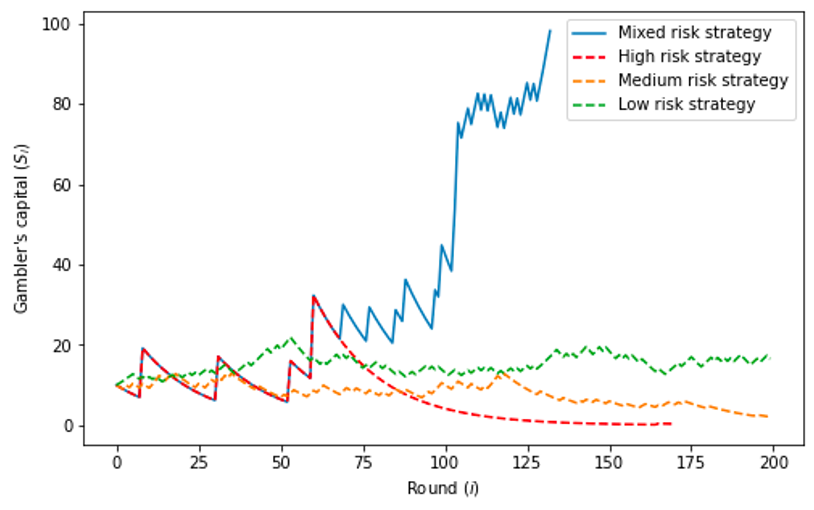
\includegraphics[width=13cm]{comparison_final.png}
        \caption[Risk adaptable strategy comparison]{\textit{Risk adaptable strategy comparison}. This figure depicts the performance of 4 distinct betting strategies: low risk, medium risk, high risk, and mixed risk, employed by four players simultaneously. Each player starts with an initial capital of 10 units and aims to achieve a profit target of 100 units. The bet amount proportion, denoted $l = 0.05$. The dynamic nature of the mixed risk strategy allows to reach the goal $G$.}\label{graf:final_graph}
\end{figure}


\section{Conclusions}\label{Conclusions}
\subsection{Main results, recommendations, limitations and further research}
In order to provide a summary of the research conducted in this dissertation, let's review the three objectives of this study, the outcomes achieved, and the suggested recommendations.

To fulfill the first objective of this work, which is to provide insights into detecting biases in the roulette wheel, we described the Pearson Chi-squared test as a statistical method for comparing expected frequencies of winning numbers with observed outcomes. In the context of European roulette, when a specific number or compartment demonstrates a positive bias, the optimal approach involves placing bets on that particular number or incorporating it into various bet types. It's worth noting that if this positive bias is equal to or higher than $(1/36 - 1/37)$, the recommendation is to employ the betting systems presented in Chapter \ref{Literature_review}, as the game turns into a favorable one from the gambler's perspective.

The second objective of this dissertation was to explore various betting strategies aimed at assisting gamblers in achieving a specific goal $G$. This exploration considered the flat betting system, proportional betting system, and Martingale betting system. Detailed algorithms were provided for their implementation. Subsequently, a comprehensive exercise was conducted to compare the performance of these strategies. The first exercise constrained strategies to earning a single monetary unit per round, while the second involved betting a fixed proportion of the available capital.

The analysis, presented in Chapter \ref{Empirical_analysis}, yielded insightful findings: for gamblers targeting 1-unit wins to reach $G$, the most effective approach involves employing the Martingale system with high-payoff bets. This choice maximizes the probability of achieving the predefined goal. On the other hand, for those prioritizing the minimization of the time required to reach $G$, the recommended strategy is to adopt the Martingale system while focusing on the lowest-risk bets.

Lastly, the third objective of this work was successfully achieved with the proposal of a risk-adaptable betting strategy specifically designed for the European roulette game. The results obtained from the exercise comparing single-risk strategies (proportional betting systems) with the mixed-risk strategy revealed a noteworthy insight. The mixed-risk strategy demonstrates a comparable estimated probability of ruin to high-risk strategies, while offering the potential to reduce the average number of rounds necessary to reach the predetermined goal $G$ (as seen in the final section of Chapter \ref{Empirical_analysis}). This strategy is recommended for individuals who are comfortable with high-risk bets.

The proposed strategy presents a practical solution for gamblers striving to minimize their playing duration and reduce potential losses. Given the inherently negative expectation nature of the roulette game, this strategy emerges as a viable option for enhancing a player’s experience and optimizing outcomes.

While the work performed in this dissertation is insightful, it also highlights certain limitations that warrant consideration. The gambling scenario employed in the empirical analysis was relatively narrow and did not encompass some practical and fundamental constraints imposed by real casinos, such as minimum and maximum betting limits. Consequently, the impact of these limitations on the effectiveness of the strategies remains unexplored. Incorporating casino-specific betting limits into the decision criteria could yield more realistic outcomes and enhance gamblers' ability to stay within feasible betting ranges. Pursuing this avenue represents a logical next step for future research.

Another limitation arises from the selection of profit milestones $\alpha_{1}$ and $\alpha_{2}$ for the proposed risk-adaptable strategy. This introduces subjectivity into the analysis, potentially resulting in varied strategy behaviors based on different milestone values. Investigating diverse setups for $\alpha_{i}$ could yield deeper insights into the behavior of the risk-adaptable strategy across various milestone configurations. Furthermore, expanding the strategy to include more than two milestones could facilitate more nuanced adaptations, potentially enhancing efficiency in achieving profit targets.

Moreover, this dissertation exclusively focuses on a specific profit goal range, which might constrain the comprehensive representation of strategy performance. Exploring alternative profit goals could yield different results and enhance the robustness of the conclusions. While the investigated strategies are informative, they represent only a subset of the possible approaches gamblers might employ. Broadening the array of strategies or adopting a more generalized approach could contribute to a more inclusive and widely applicable set of insights.

Another important aspect to consider is the average amount of money that a gambler might lose before successfully reaching their goal. While achieving the goal is the main objective, it's also crucial to assess the potential losses incurred along the way. This concept delves into the notion of risk tolerance and the financial implications of pursuing the established goal. For instance, a strategy that reaches the goal quickly but involves significant losses in the process might not be preferable to a more conservative approach that incurs smaller losses but takes longer to achieve the goal. Balancing the trade-off between reaching the goal swiftly and managing potential losses is a nuanced consideration that can significantly impact the choice of a betting strategy. Therefore, a comprehensive evaluation of different strategies should take into account not only the probability of reaching $G$ but also the associated financial risks encountered before reaching $G$.

Finally, hybrid approaches that combine multiple strategies are a promising avenue for future research in the field of betting strategies, not only for the roulette case but also for more general casino games. These hybrid strategies could potentially leverage the strengths of different strategies while mitigating their individual weaknesses. For instance, combining elements of the Martingale strategy with a mixture of low, medium, and high bet types. Incorporating elements of the Martingale strategy to switch to lower-risk bets after a certain threshold of accumulated losses could help manage risk and prevent the complete depletion of capital. In this case, the milestones would be associated with the accumulated losses rather than the proportion of the goal reached.

\subsection{Final reflections}
The proposed risk-adapted strategy shares resemblances with real-life stock market investments in certain aspects, particularly in terms of risk management and the adjustment of strategies based on profit targets. When an investor sets a high-profit target relative to their initial capital, achieving it through conservative investments may require an impractically long time. To accelerate capital growth, some investors might initiate with high-risk assets or stocks, aiming for rapid increases. As they approach their profit goal, they may transition to more conservative investments to safeguard their gains and avoid substantial losses. 

However, it's important to note that investing in the stock market involves various considerations, including long-term perspectives and risk diversification. Stock market investment is far more complex than gambling due to the absence of the independence assumption. In gambling, each round of play, such as spinning the roulette wheel, remains independent of previous and future rounds. The outcome of one spin has no impact on the outcome of the next. In contrast, the stock market is characterized by an intricate web of interconnections and relationships between various assets and economic factors. Stock prices are influenced by company performance, economic indicators, geopolitical events, among other factors.

While this analogy can illustrate the intricate nature of financial markets and the interdependence of various factors, it's essential to remember that real stock market investing involves analysis and long-term planning. The outcomes of investments in the stock market are not purely based on chance, as in gambling, but are influenced by real-world events and the underlying value and performance of the traded assets. Thus, while analogies can be helpful for understanding certain aspects, stock market investing remains a more complex and strategic endeavor than gambling on a roulette wheel.

Another, and perhaps the most important, reflection of this work is that the usage of any betting system does not change the probabilities of winning, losing, or tying in each round of a game. However, these systems may potentially enhance the likelihood of short-term wins only. There is a distinction between the short-term and long-term impact of betting systems that readers, gamblers, or other researchers need to clearly understand.

In the short term, betting systems may give the illusion of success due to the natural fluctuations in random outcomes. A player using a betting system might experience a winning streak and see their capital increase, leading them to believe that the system is effective. However, these short-term gains are often temporary and driven by chance rather than the betting strategy itself. On the other hand, in the long term, the Law of Large Numbers comes into play. This statistical principle states that as the number of trials increases, the actual results will converge to the expected probabilities. In games of chance, where the odds are fixed and independent for each trial, the expected outcomes remain the same, regardless of the betting system used.

Betting systems themselves do not affect the fundamental nature of the game, but they can influence certain aspects related to the player's experience. For example, the duration of the game and the likelihood of achieving a specific increase in capital (or incurring a loss) can be influenced by the betting system. In other words, even though the game's inherent fairness remains the same, the betting system can impact how long a player can sustain their bets before running out of funds or reaching their desired profit target. It can also affect the probability of achieving a certain level of wealth increase while accepting the risk of losing money.
\clearpage


\bibliography{literature}
\clearpage




\appendix
%\addcontentsline{toc}{section}{Appendices}

\section{Appendix Smart Live Casino data}
\vspace{3em}
\begin{sideways}
\begin{minipage}[b]{0.9\textheight}
\captionof{table}{Smart Live Casino data}
  \small
  \label{tab:casino_data}
  \begin{tabular}{|*{30}{c|}}
     \hline
     \multicolumn{30}{|c|}{\textbf{Image}}\\ 
      \hline
    \textbf{1} &\textbf{2} &\textbf{3} &\textbf{4} &\textbf{5}&\textbf{6}&7 &\textbf{8} &\textbf{9} &\textbf{10} &\textbf{11} &\textbf{12} &\textbf{13} &1\textbf{4} &\textbf{15}&\textbf{16} &\textbf{17} &\textbf{18} &\textbf{19} &\textbf{20} &\textbf{21} &\textbf{22} &\textbf{23}&\textbf{24} &\textbf{25} &\textbf{26} &\textbf{27} &\textbf{28} &\textbf{29} &\textbf{30}\\
    \hline
    \hline
6 &21 &9 &19 &27 &10 &25 &8 &31 &25 &27 &14 &33 &30 &8&8 &22 &3 &25 &32 &32 &16 &20 &26 &7 &0 &4 &19 &23 &9\\
1 &6 &22 &33 &10 &36 &13 &19 &29 &4 &18 &6 &21 &10 &28&13 &34 &31 &1 &5 &2 &7 &25 &34 &5 &12 &8 &13 &16 &25\\
22 &25 &33 &22 &34 &9 &32 &6 &35 &29 &0 &29 &17 &10 &18&22 &25 &12 &17 &19 &6 &30 &25 &28 &29 &15 &28 &27 &32 &24\\
11 &10 &23 &31 &28 &17 &9 &17 &35 &34 &32 &26 &22 &24 &2&5 &14 &24 &29 &12 &9 &22 &12 &11 &18 &28 &9 &11 &3 &19\\
25 &29 &25 &12 &33 &3 &30 &9 &12 &0 &24 &35 &24 &13 &33&13 &11 &6 &32 &23 &34 &6 &16 &26 &1 &31 &26 &2 &7 &29\\
14 &23 &14 &1 &4 &26 &21 &35 &21 &0 &17 &18 &32 &14 &5&24 &10 &12 &29 &21 &32 &36 &19 &32 &15 &31 &29 &13 &13 &7\\
36 &31 &23 &20 &16 &20 &27 &9 &14 &6 &30 &14 &10 &20 &23&25 &4 &2 &7 &6 &25 &10 &10 &26 &10 &2 &35 &21 &32 &9\\
17 &12 &7 &36 &26 &21 &10 &30 &20 &11 &14 &4 &9 &13 &36&22 &4 &17 &35 &9 &4 &2 &29 &22 &18 &29 &20 &12 &11 &30\\
17 &18 &26 &19 &19 &18 &4 &10 &24 &12 &21 &27 &15 &4 &23&18 &24 &1 &14 &15 &10 &30 &2 &26 &12 &33 &19 &18 &9 &15\\
10 &21 &34 &20 &36 &33 &36 &4 &26 &23 &32 &15 &21 &28 &28&4 &10 &12 &22 &12 &33 &30 &25 &28 &28 &16 &24 &36 &12 &7\\
18 &24 &17 &4 &11 &29 &13 &28 &5 &33 &1 &21 &22 &32 &1&32 &3 &33 &20 &32 &31 &10 &36 &29 &7 &13 &32 &15 &20 &17\\
1 &20 &6 &15 &35 &6 &2 &32 &28 &22 &35 &36 &27 &3 &0&32 &7 &19 &22 &36 &12 &36 &29 &26 &15 &6 &19 &32 &27 &25\\
10 &28 &13 &7 &28 &33 &4 &2 &27 &9 &13 &10 &1 &1 &32&6 &5 &17 &23 &16 &36 &23 &35 &0 &14 &27 &2 &33 &29 &19\\
22 &17 &8 &35 &33 &1 &9 &36 &3 &35 &5 &18 &1 &31 &34&9 &5 &29 &9 &29 &32 &12 &21 &35 &26 &13 &29 &22 &13 &26\\
16 &6 &20 &19 &9 &36 &26 &21 &17 &26 &30 &24 &19 &12 &33&23 &5 &4 &23 &27 &31 &26 &27 &19 &27 &32 &22 &19 &30 &18\\
33 &26 &26 &35 &5 &11 &11 &0 &5 &16 &5 &2 &20 &36 &16&21 &15 &23 &8 &36 &16 &36 &15 &15 &2 &19 &30 &7 &34 &25\\
6 &0 &12 &31 &21 &35 &13 &27 &2 &6 &8 &36 &35 &23 &11&14 &18 &16 &19 &22 &34 &36 &26 &20 &7 &35 &2 &22 &4 &17\\
35 &5 &33 &34 &11 &34 &10 &4 &20 &30 &13 &14 &15 &8 &5&8 &20 &5 &35 &32 &10 &13 &22 &21 &28 &14 &33 &12 &5 &25\\
7 &20 &11 &13 &17 &7 &8 &18 &12 &1 &33 &27 &7 &18 &3&26 &24 &13 &2 &27 &27 &31 &17 &11 &0 &13 &31 &26 &2 &29\\
18 &33 &9 &14 &15 &13 &22 &23 &17 &2 &34 &17 &36 &11 &14&17 &33 &0 &18 &28 &27 &20 &36 &13 &31 &14 &21 &32 &20 &10\\
28 &36 &34 &35 &18 &12 &28 &25 &29 &12 &23 &20 &11 &19 &29&27 &36 &7 &19 &9 &1 &16 &28 &8 &6 &10 &12 &5 &14 &22\\
9 &22 &6 &13 &3 &6 &34 &1 &14 &30 &33 &6 &35 &20 &14&13 &2 &34 &3 &8 &26 &17 &5 &34 &6 &13 &32 &1 &14 &5\\
2 &16 &14 &35 &15 &21 &35 &2 &10 &20 &1 &4 &22 &23 &3&13 &28 &19 &3 &29 &34 &13 &26 &28 &20 &25 &19 &25 &34 &7\\
23 &15 &34 &19 &20 &11 &12 &15 &33 &25 &13 &36 &13 &15 &22&10 &0 &27 &35 &5 &3 &30 &8 &28 &8 &3 &34 &9 &18 &14\\
4 &28 &3 &29 &7 &8 &2 &3 &7 &16 &3 &33 &26 &9 &29&20 &30 &24 &22 &21 &32 &17 &21 &9 &11 &27 &28 &10 &2 &26\\
23 &29 &30 &20 &31 &19 &31 &15 &17 &33 &6 &36 &0 &18 &20&17 &10 &16 &32 &26 &8 &29 &25 &2 &3 &0 &10 &35 &19 &0\\
2 &28 &9 &20 &32 &10 &21 &23 &32 &17 &34 &33 &1 &9 &30&14 &5 &12 &22 &15 &29 &15 &22 &0 &6 &21 &27 &36 &7 &20\\
31 &19 &27 &31 &1 &27 &35 &6 &28 &10 &0 &19 &6 &20 &33&28 &35 &32 &17 &32 &21 &0 &8 &14 &18 &27 &27 &10 &29 &16\\
29 &17 &32 &1 &27 &8 &23 &23 &29 &32 &16 &25 &6 &21 &22&2 &16 &19 &3 &5 &17 &16 &25 &13 &22 &7 &23 &25 &11 &5\\
17 &20 &12 &7 &12 &27 &6 &21 &32 &30 &13 &29 &8 &25 &24&10 &21 &23 &18 &2 &26 &26 &3 &15 &7 &13 &17 &14 &24 &0\\
36 &16 &9 &34 &12 &35 &22 &15 &11 &16 &34 &18 &35 &21 &36&1 &9 &17 &7 &7 &17 &33 &12 &22 &6 &25 &33 &33 &2 &12\\
  \hline
    \multicolumn{30}{r}{Continues on the next page} \\
      \end{tabular}
      \end{minipage}
\end{sideways}


\begin{sidewaystable}
  \small
  \begin{tabular}{|*{30}{c|}}
    \hline
     \multicolumn{30}{|c|}{\textbf{Image}} \\
     \hline
    \textbf{1} &\textbf{2} &\textbf{3} &\textbf{4} &\textbf{5}&\textbf{6}&7 &\textbf{8} &\textbf{9} &\textbf{10} &\textbf{11} &\textbf{12} &\textbf{13} &1\textbf{4} &\textbf{15}&\textbf{16} &\textbf{17} &\textbf{18} &\textbf{19} &\textbf{20} &\textbf{21} &\textbf{22} &\textbf{23}&\textbf{24} &\textbf{25} &\textbf{26} &\textbf{27} &\textbf{28} &\textbf{29} &\textbf{30}\\
    \hline
    \hline
36 &34 &21 &9 &18 &27 &24 &8 &16 &29 &3 &27 &35 &14 &5&12 &33 &22 &23 &34 &9 &9 &26 &18 &22 &8 &15 &27 &11 &28\\
27 &5 &1 &18 &30 &19 &4 &33 &6 &19 &28 &2 &27 &27 &18&35 &31 &15 &2 &23 &27 &4 &22 &23 &18 &12 &31 &25 &33 &2\\
5 &25 &9 &12 &35 &35 &8 &9 &36 &22 &0 &6 &20 &8 &2&11 &25 &4 &10 &17 &21 &34 &16 &28 &1 &15 &28 &23 &28 &19\\
1 &12 &23 &3 &20 &11 &16 &0 &17 &3 &2 &27 &14 &29 &23&15 &31 &27 &7 &31 &21 &1 &1 &34 &16 &34 &24 &15 &2 &23\\
30 &24 &9 &35 &19 &28 &30 &7 &21 &1 &0 &1 &29 &3 &2&19 &12 &11 &0 &16 &31 &36 &31 &35 &30 &5 &21 &9 &9 &11\\
26 &5 &28 &27 &15 &31 &31 &18 &2 &32 &6 &3 &19 &0 &8&11 &8 &36 &19 &30 &18 &30 &14 &15 &19 &6 &29 &15 &23 &33\\
19 &13 &28 &19 &22 &27 &36 &28 &26 &23 &22 &5 &35 &34 &30&23 &3 &21 &31 &29 &19 &1 &5 &24 &15 &21 &35 &29 &4 &26\\
17 &31 &2 &34 &26 &23 &31 &10 &17 &18 &33 &17 &15 &26 &29&22 &21 &6 &12 &36 &34 &33 &3 &28 &2 &1 &17 &8 &31 &15\\
1 &36 &28 &0 &22 &33 &13 &30 &28 &11 &23 &17 &28 &20 &11&9 &27 &36 &20 &12 &11 &25 &34 &20 &15 &10 &30 &23 &23 &9\\
16 &27 &11 &17 &29 &12 &4 &22 &26 &33 &27 &2 &3 &18 &16&10 &32 &4 &31 &17 &36 &24 &12 &4 &23 &9 &4 &30 &27 &4\\
29 &32 &10 &11 &33 &7 &21 &7 &4 &18 &26 &32 &14 &1 &29&14 &29 &28 &8 &23 &36 &3 &24 &25 &0 &27 &5 &10 &26 &20\\
30 &12 &23 &22 &5 &14 &8 &25 &35 &21 &6 &0 &4 &6 &24&3 &23 &15 &13 &9 &23 &12 &26 &8 &17 &34 &8 &12 &26 &34\\
24 &1 &5 &1 &18 &20 &23 &12 &3 &7 &13 &29 &9 &2 &24&26 &16 &35 &15 &3 &17 &12 &14 &30 &23 &27 &6 &23 &35 &13\\
7 &3 &24 &4 &35 &32 &7 &7 &21 &35 &33 &19 &29 &5 &10&32 &35 &26 &32 &17 &3 &1 &15 &5 &27 &31 &12 &31 &24 &30\\
29 &25 &32 &9 &22 &20 &11 &1 &13 &27 &7 &35 &8 &23 &27&13 &32 &35 &5 &0 &23 &4 &31 &19 &26 &18 &12 &31 &6 &12\\
10 &6 &27 &20 &9 &1 &28 &16 &11 &23 &20 &12 &20 &14 &2&2 &5 &14 &31 &13 &17 &11 &16 &6 &12 &22 &33 &2 &18 &24\\
28 &18 &27 &29 &33 &9 &21 &9 &14 &35 &3 &10 &7 &0 &20&0 &32 &11 &0 &15 &2 &33 &0 &20 &33 &8 &7 &26 &7 &9\\
13 &9 &23 &26 &15 &5 &16 &16 &27 &18 &31 &36 &32 &7 &4&21 &5 &36 &5 &36 &20 &6 &19 &1 &18 &36 &35 &32 &23 &0\\
11 &33 &34 &11 &32 &6 &7 &21 &32 &23 &17 &16 &5 &9 &19&10 &0 &29 &19 &12 &10 &30 &36 &20 &13 &22 &10 &6 &18 &15\\
0 &10 &5 &23 &18 &18 &8 &2 &17 &36 &3 &34 &9 &6 &22&13 &14 &0 &10 &35 &20 &28 &26 &17 &36 &22 &26 &1 &14 &33\\
16 &14 &30 &21 &22 &3 &24 &12 &17 &29 &22 &30 &1 &36 &33&20 &10 &18 &29 &23 &8 &34 &34 &30 &9 &14 &13 &30 &2 &20\\
30 &28 &35 &36 &9 &21 &12 &3 &36 &15 &18 &2 &36 &23 &27&13 &31 &34 &20 &9 &10 &20 &24 &10 &7 &33 &7 &21 &25 &2\\
22 &12 &33 &25 &20 &23 &25 &14 &21 &17 &28 &1 &5 &10 &36&9 &27 &24 &32 &5 &10 &21 &4 &8 &2 &35 &6 &14 &1 &3\\
10 &31 &12 &34 &5 &7 &2 &13 &21 &8 &28 &11 &29 &0 &28&30 &5 &1 &12 &19 &7 &26 &11 &19 &32 &10 &9 &19 &30 &15\\
13 &16 &6 &19 &5 &29 &27 &12 &33 &30 &25 &17 &28 &21 &35&24 &8 &13 &29 &16 &34 &18 &4 &29 &36 &33 &15 &36 &30 &31\\
2 &4 &10 &36 &5 &2 &22 &13 &5 &26 &5 &5 &9 &9 &18&11 &8 &23 &0 &12 &0 &13 &32 &30 &0 &15 &18 &5 &28 &27\\
10 &18 &34 &4 &3 &33 &21 &14 &16 &2 &2 &13 &2 &29 &26&1 &8 &14 &25 &6 &2 &2 &6 &25 &3 &33 &21 &0 &30 &14\\
21 &24 &35 &1 &14 &29 &0 &17 &22 &24 &6 &11 &28 &12 &4&5 &25 &26 &16 &28 &29 &31 &10 &2 &19 &31 &0 &21 &17 &29\\
24 &14 &13 &10 &29 &26 &23 &14 &32 &15 &0 &15 &9 &24 &8&20 &10 &28 &5 &32 &5 &1 &4 &0 &4 &6 &24 &34 &18 &0\\
29 &23 &13 &8 &12 &24 &12 &21 &17 &34 &13 &14 &25 &30 &29&34 &21 &31 &2 &27 &11 &2 &34 &21 &3 &29 &14 &30 &30 &7\\
36 &11 &30 &20 &30 &23 &15 &29 &19 &10 &18 &29 &23 &31 &33&22 &31 &36 &2 &35 &14 &15 &32 &21 &30 &11 &33 &27 &26 &25\\
5 &21 &2 &1 &21 &17 &18 &31 &7 &16 &30 &5 &22 &29 &18&4 &26 &12 &17 &36 &35 &12 &7 &25 &13 &10 &9 &5 &3 &14\\
11 &5 &29 &21 &2 &25 &15 &31 &12 &15 &27 &7 &19 &24 &14&0 &26 &13 &15 &25 &0 &22 &2 &23 &20 &30 &0 &12 &20 &32\\
  \hline
    \multicolumn{30}{r}{Continues on the next page} \\
      \end{tabular}
      \end{sidewaystable}
      
\begin{sidewaystable}
  \small
  \begin{tabular}{|*{30}{c|}}
    \hline
     \multicolumn{30}{|c|}{\textbf{Image}} \\
     \hline
    \textbf{1} &\textbf{2} &\textbf{3} &\textbf{4} &\textbf{5}&\textbf{6}&7 &\textbf{8} &\textbf{9} &\textbf{10} &\textbf{11} &\textbf{12} &\textbf{13} &1\textbf{4} &\textbf{15}&\textbf{16} &\textbf{17} &\textbf{18} &\textbf{19} &\textbf{20} &\textbf{21} &\textbf{22} &\textbf{23}&\textbf{24} &\textbf{25} &\textbf{26} &\textbf{27} &\textbf{28} &\textbf{29} &\textbf{30}\\
    \hline
    \hline
30 &0 &35 &6 &33 &22 &2 &2 &33 &20 &28 &7 &3 &9 &3&19 &15 &8 &29 &14 &10 &35 &17 &33 &34 &0 &35 &29 &23 &16\\
2 &1 &12 &12 &7 &22 &4 &6 &30 &23 &9 &30 &25 &8 &36&34 &34 &28 &26 &10 &6 &24 &4 &10 &18 &19 &21 &7 &11 &20\\
11 &29 &28 &17 &2 &27 &35 &11 &14 &19 &27 &2 &26 &22 &33&26 &9 &18 &1 &36 &18 &4 &20 &26 &23 &20 &23 &2 &26 &1\\
15 &26 &7 &1 &33 &29 &20 &0 &5 &7 &11 &3 &28 &21 &11&0 &1 &15 &2 &3 &32 &19 &6 &4 &5 &20 &11 &23 &4 &31\\
14 &9 &9 &14 &12 &20 &18 &24 &32 &23 &27 &5 &7 &0 &20&19 &35 &20 &19 &9 &28 &17 &29 &10 &21 &34 &5 &16 &1 &7\\
16 &1 &25 &2 &18 &32 &31 &24 &14 &21 &31 &10 &33 &26 &18&33 &33 &32 &20 &25 &17 &22 &17 &17 &30 &18 &27 &4 &29 &7\\
13 &3 &26 &20 &26 &0 &9 &11 &36 &16 &23 &22 &12 &14 &1&22 &8 &0 &13 &1 &6 &17 &33 &8 &24 &16 &14 &30 &33 &32\\
9 &22 &10 &12 &8 &2 &32 &8 &1 &8 &24 &6 &36 &27 &13&2 &36 &3 &20 &8 &33 &25 &30 &10 &34 &3 &18 &36 &3 &31\\
0 &12 &1 &10 &3 &12 &33 &34 &16 &25 &3 &20 &3 &4 &13&1 &22 &1 &21 &17 &6 &2 &29 &13 &13 &11 &25 &8 &0 &19\\
34 &2 &31 &34 &11 &35 &16 &16 &19 &25 &28 &14 &24 &14 &30&31 &36 &18 &15 &26 &17 &16 &31 &9 &20 &21 &28 &30 &31 &19\\
24 &27 &32 &33 &15 &28 &14 &3 &32 &32 &16 &3 &2 &22 &5&29 &5 &24 &30 &22 &14 &28 &6 &16 &10 &16 &26 &36 &22 &19\\
29 &20 &22 &8 &25 &30 &16 &33 &11 &32 &23 &5 &5 &31 &5&16 &3 &20 &7 &26 &10 &19 &27 &31 &32 &0 &36 &2 &16 &1\\
33 &16 &30 &9 &11 &18 &26 &22 &0 &3 &6 &29 &16 &31 &8&26 &9 &30 &25 &1 &27 &8 &22 &8 &36 &15 &20 &32 &11 &1\\
0 &17 &12 &22 &8 &28 &26 &10 &34 &1 &1 &2 &10 &1 &18&9 &3 &19 &8 &7 &34 &10 &14 &16 &29 &34 &21 &25 &33 &6\\
36 &8 &0 &33 &24 &1 &35 &35 &14 &16 &22 &23 &21 &9 &3&1 &1 &33 &26 &16 &14 &19 &12 &36 &29 &35 &17 &18 &22 &29\\
25 &10 &9 &23 &6 &36 &4 &14 &13 &34 &3 &13 &24 &13 &35&23 &34 &27 &20 &15 &34 &9 &20 &1 &9 &21 &33 &26 &31 &2\\
9 &0 &20 &25 &28 &4 &31 &16 &9 &9 &5 &17 &23 &7 &3&36 &17 &29 &3 &3 &9 &32 &31 &13 &25 &2 &25 &2 &34 &24\\
23 &13 &0 &14 &17 &14 &32 &4 &19 &33 &24 &8 &17 &10 &16&17 &22 &8 &9 &10 &23 &17 &29 &31 &20 &4 &6 &27 &36 &34\\
19 &17 &2 &23 &19 &16 &18 &34 &22 &6 &1 &19 &36 &7 &36&19 &18 &18 &27 &6 &29 &13 &27 &6 &13 &13 &14 &11 &2 &23\\
7 &20 &8 &7 &31 &7 &16 &27 &21 &20 &36 &8 &29 &23 &17&29 &14 &23 &10 &36 &33 &30 &17 &12 &26 &6 &1 &9 &32 &26\\
28 &34 &24 &26 &17 &24 &3 &4 &15 &23 &5 &29 &3 &12 &23&29 &13 &6 &3 &27 &10 &9 &25 &32 &15 &9 &9 &5 &22 &12\\
24 &11 &27 &34 &14 &36 &21 &1 &11 &34 &13 &26 &20 &10 &15&33 &18 &25 &1 &1 &11 &13 &20 &18 &13 &17 &17 &29 &5 &0\\
24 &33 &34 &17 &24 &14 &7 &13 &4 &21 &34 &31 &30 &12 &19&16 &1 &26 &20 &0 &27 &6 &31 &19 &14 &23 &28 &21 &8 &22\\
24 &29 &19 &6 &33 &3 &31 &32 &23 &18 &5 &18 &34 &4 &1&13 &8 &28 &15 &18 &34 &27 &10 &36 &25 &20 &26 &34 &25 &19\\
5 &15 &6 &13 &26 &8 &33 &30 &7 &7 &10 &25 &22 &27 &24&34 &13 &19 &35 &32 &29 &18 &15 &15 &13 &2 &36 &36 &34 &6\\
9 &26 &9 &8 &31 &29 &17 &33 &11 &4 &25 &23 &27 &35 &28&5 &14 &28 &4 &5 &14 &7 &25 &36 &3 &1 &16 &4 &16 &20\\
18 &2 &34 &20 &34 &13 &2 &17 &34 &29 &19 &5 &1 &5 &18&30 &24 &20 &16 &19 &36 &10 &35 &9 &13 &19 &22 &1 &10 &2\\
21 &25 &7 &26 &11 &36 &0 &25 &34 &36 &13 &4 &29 &25 &1&21 &32 &7 &34 &4 &23 &3 &18 &22 &29 &10 &9 &20 &14 &14\\
36 &7 &29 &12 &27 &6 &7 &7 &32 &6 &35 &29 &9 &8 &27&4 &24 &33 &9 &33 &28 &17 &21 &5 &1 &2 &9 &36 &32 &9\\
3 &31 &36 &33 &5 &9 &17 &8 &0 &16 &1 &33 &7 &15 &1&3 &25 &36 &15 &21 &0 &14 &29 &36 &6 &3 &33 &22 &24 &33\\
8 &9 &33 &11 &28 &17 &35 &0 &33 &21 &26 &19 &34 &30 &12&26 &3 &1 &2 &18 &7 &9 &24 &17 &19 &32 &4 &33 &11 &24\\
25 &32 &6 &9 &34 &30 &27 &32 &33 &36 &23 &4 &6 &31 &4&12 &17 &21 &23 &24 &33 &12 &16 &28 &29 &16 &27 &17 &25 &13\\
  \hline
    \multicolumn{30}{r}{Continues on the next page} \\
      \end{tabular}
\end{sidewaystable}

\begin{sidewaystable}
  \small
  \begin{tabular}{|*{30}{c|}}
    \hline
     \multicolumn{30}{|c|}{\textbf{Image}} \\
     \hline
    \textbf{1} &\textbf{2} &\textbf{3} &\textbf{4} &\textbf{5}&\textbf{6}&7 &\textbf{8} &\textbf{9} &\textbf{10} &\textbf{11} &\textbf{12} &\textbf{13} &1\textbf{4} &\textbf{15}&\textbf{16} &\textbf{17} &\textbf{18} &\textbf{19} &\textbf{20} &\textbf{21} &\textbf{22} &\textbf{23}&\textbf{24} &\textbf{25} &\textbf{26} &\textbf{27} &\textbf{28} &\textbf{29} &\textbf{30}\\
    \hline
    \hline
20 &24 &8 &34 &6 &12 &30 &27 &19 &10 &26 &0 &0 &31 &35&19 &32 &6 &3 &12 &6 &30 &33 &36 &5 &1 &7 &23 &26 &22\\
27 &0 &28 &6 &12 &30 &17 &23 &21 &12 &31 &14 &11 &18 &26&22 &7 &1 &14 &19 &22 &15 &0 &12 &11 &18 &24 &27 &2 &7\\
2 &24 &24 &14 &12 &18 &26 &29 &29 &17 &36 &4 &19 &17 &33&14 &12 &19 &31 &9 &30 &32 &23 &17 &36 &2 &34 &26 &12 &19\\
7 &14 &34 &34 &30 &1 &21 &19 &29 &29 &13 &2 &21 &26 &23&17 &11 &14 &33 &17 &17 &32 &13 &14 &28 &28 &21 &28 &23 &0\\
36 &26 &9 &3 &30 &13 &12 &16 &11 &36 &1 &34 &20 &4 &25&19 &31 &23 &13 &36 &33 &33 &13 &10 &33 &31 &13 &3 &3 &30\\
8 &5 &23 &30 &1 &12 &10 &34 &3 &17 &22 &20 &35 &19 &28&26 &21 &31 &17 &30 &26 &24 &12 &14 &11 &2 &0 &15 &35 &0\\
23 &9 &1 &9 &19 &3 &32 &16 &12 &12 &24 &24 &31 &25 &35&33 &12 &2 &0 &34 &1 &7 &2 &19 &4 &26 &1 &15 &17 &3\\
17 &13 &9 &27 &14 &4 &14 &24 &34 &24 &11 &2 &1 &7 &26&6 &16 &21 &33 &3 &29 &32 &11 &1 &7 &20 &26 &24 &22 &34\\
9 &36 &10 &32 &3 &24 &8 &20 &27 &28 &29 &25 &35 &21 &32&14 &23 &31 &9 &28 &30 &20 &32 &24 &6 &5 &27 &34 &0 &17\\
21 &36 &12 &12 &28 &31 &35 &27 &31 &13 &36 &10 &3 &33 &26&12 &20 &22 &34 &19 &12 &10 &17 &30 &31 &28 &1 &29 &31 &2\\
15 &3 &25 &9 &4 &30 &15 &10 &13 &19 &14 &32 &28 &31 &12&31 &12 &17 &20 &24 &15 &33 &28 &19 &10 &7 &8 &14 &9 &8\\
26 &28 &5 &21 &13 &36 &29 &10 &13 &7 &19 &24 &30 &26 &5&35 &11 &19 &18 &6 &7 &25 &17 &33 &15 &13 &8 &20 &26 &17\\
8 &23 &21 &1 &18 &13 &8 &14 &4 &22 &25 &36 &18 &27 &20&15 &4 &4 &3 &1 &12 &19 &7 &9 &6 &25 &19 &24 &5 &16\\
25 &36 &9 &9 &17 &32 &9 &2 &16 &0 &18 &6 &34 &3 &1&22 &31 &3 &18 &7 &29 &21 &22 &12 &13 &9 &5 &34 &36 &31\\
17 &32 &21 &23 &33 &3 &12 &25 &20 &25 &12 &12 &32 &22 &13&19 &26 &10 &20 &4 &23 &9 &30 &8 &27 &20 &9 &7 &15 &22\\
17 &2 &11 &9 &17 &32 &31 &8 &9 &32 &9 &12 &24 &1 &1&21 &30 &28 &8 &29 &36 &18 &24 &23 &34 &12 &34 &11 &8 &25\\
18 &15 &23 &28 &28 &5 &26 &8 &13 &35 &29 &16 &25 &26 &15&23 &25 &16 &25 &28 &14 &19 &20 &15 &30 &17 &24 &9 &20 &23\\
35 &4 &8 &28 &19 &33 &16 &23 &22 &13 &31 &35 &17 &11 &11&19 &21 &11 &33 &3 &10 &31 &19 &11 &3 &16 &31 &2 &25 &34\\
25 &12 &28 &2 &11 &22 &35 &20 &26 &11 &18 &26 &22 &33 &15&2 &15 &34 &36 &19 &20 &14 &7 &25 &11 &25 &5 &27 &14 &22\\
26 &2 &22 &28 &6 &36 &4 &36 &33 &2 &35 &25 &18 &17 &11&14 &26 &3 &27 &4 &16 &27 &20 &11 &7 &22 &35 &33 &16 &16\\
0 &19 &18 &11 &29 &29 &23 &23 &15 &6 &11 &27 &35 &13 &9&20 &17 &1 &16 &8 &10 &28 &36 &27 &4 &12 &1 &21 &34 &0\\
4 &29 &14 &10 &9 &7 &8 &23 &17 &0 &36 &12 &9 &29 &34&11 &26 &33 &21 &5 &7 &29 &27 &6 &21 &29 &17 &13 &2 &33\\
34 &0 &1 &23 &28 &20 &23 &18 &18 &2 &31 &22 &25 &33 &0&20 &25 &8 &31 &22 &9 &18 &30 &20 &9 &14 &8 &27 &10 &3\\
16 &0 &5 &5 &7 &8 &27 &1 &0 &35 &10 &0 &21 &28 &12&22 &36 &24 &27 &5 &36 &31 &34 &13 &29 &23 &26 &7 &29 &4\\
29 &30 &35 &24 &15 &26 &31 &25 &28 &3 &7 &1 &21 &23 &24&12 &15 &30 &9 &13 &4 &36 &26 &8 &14 &0 &6 &18 &1 &0\\
11 &16 &7 &32 &26 &5 &10 &8 &9 &21 &10 &34 &11 &1 &8&8 &4 &28 &26 &29 &21 &10 &16 &13 &14 &1 &1 &22 &21 &27\\
5 &29 &15 &27 &24 &12 &11 &36 &0 &6 &25 &34 &16 &17 &22&11 &11 &31 &23 &26 &15 &19 &10 &34 &8 &17 &33 &2 &27 &7\\
27 &19 &3 &27 &26 &21 &26 &9 &31 &6 &14 &17 &2 &10 &0&9 &23 &12 &15 &7 &12 &16 &14 &8 &20 &31 &34 &33 &24 &31\\
23 &24 &1 &23 &11 &32 &14 &2 &14 &6 &21 &24 &23 &22 &2&6 &34 &34 &18 &30 &6 &15 &21 &36 &32 &14 &12 &15 &18 &21\\
20 &15 &0 &34 &8 &16 &17 &31 &8 &22 &4 &6 &2 &7 &13&11 &21 &1 &32 &0 &28 &0 &32 &27 &11 &35 &21 &14 &18 &2\\
34 &35 &32 &5 &8 &31 &3 &29 &17 &18 &15 &20 &14 &7 &7&28 &27 &19 &15 &7 &16 &23 &1 &13 &7 &35 &1 &9 &26 &22\\
19 &28 &4 &30 &36 &26 &32 &20 &19 &12 &1 &24 &14 &1 &11&6 &26 &1 &36 &12 &4 &21 &10 &30 &18 &11 &4 &8 &6 &30\\
  \hline
    \multicolumn{30}{r}{Continues on the next page} \\
      \end{tabular}
\end{sidewaystable}

\begin{sidewaystable}
  \small
  \begin{tabular}{|*{30}{c|}}
    \hline
     \multicolumn{30}{|c|}{\textbf{Image}} \\
     \hline
    \textbf{1} &\textbf{2} &\textbf{3} &\textbf{4} &\textbf{5}&\textbf{6}&7 &\textbf{8} &\textbf{9} &\textbf{10} &\textbf{11} &\textbf{12} &\textbf{13} &1\textbf{4} &\textbf{15}&\textbf{16} &\textbf{17} &\textbf{18} &\textbf{19} &\textbf{20} &\textbf{21} &\textbf{22} &\textbf{23}&\textbf{24} &\textbf{25} &\textbf{26} &\textbf{27} &\textbf{28} &\textbf{29} &\textbf{30}\\
    \hline
    \hline
11 &22 &32 &35 &30 &14 &31 &28 &33 &29 &29 &32 &34 &33 &24&32 &36 &23 &34 &15 &22 &29 &24 &35 &2 &3 &6 &31 &14 &19\\
24 &10 &21 &33 &34 &22 &10 &13 &33 &9 &17 &27 &10 &34 &8&29 &26 &9 &12 &20 &32 &24 &21 &23 &13 &8 &27 &14 &13 &3\\
19 &25 &30 &12 &8 &27 &5 &6 &25 &30 &4 &19 &6 &24 &12&29 &21 &15 &10 &6 &10 &30 &35 &27 &20 &9 &0 &36 &36 &5\\
22 &36 &25 &6 &28 &16 &14 &17 &25 &2 &22 &7 &22 &8 &32&4 &29 &20 &28 &26 &1 &15 &12 &20 &0 &7 &16 &34 &28 &18\\
2 &34 &17 &10 &10 &6 &36 &3 &18 &12 &35 &20 &28 &0 &29&19 &2 &3 &33 &15 &9 &5 &13 &33 &19 &19 &20 &10 &12 &31\\
22 &27 &0 &34 &35 &35 &3 &32 &14 &22 &17 &2 &29 &20 &27&24 &29 &34 &35 &31 &33 &34 &0 &28 &14 &33 &17 &9 &23 &21\\
32 &35 &26 &35 &30 &18 &13 &0 &12 &31 &36 &29 &29 &18 &26&7 &2 &31 &3 &32 &32 &6 &0 &19 &14 &2 &8 &8 &30 &35\\
35 &27 &24 &13 &15 &24 &19 &27 &27 &17 &6 &28 &14 &34 &10&3 &3 &28 &0 &6 &4 &2 &19 &33 &8 &35 &0 &8 &34 &15\\
5 &16 &7 &13 &30 &25 &2 &10 &21 &27 &27 &1 &24 &24 &21&7 &13 &35 &22 &36 &11 &11 &19 &2 &23 &28 &11 &1 &4 &1\\
2 &19 &15 &30 &9 &31 &24 &28 &2 &21 &28 &31 &9 &0 &35&24 &32 &6 &8 &26 &17 &14 &31 &19 &12 &18 &8 &20 &13 &31\\
24 &2 &27 &2 &7 &0 &5 &10 &34 &18 &36 &11 &27 &33 &8&30 &27 &13 &20 &20 &29 &7 &25 &3 &10 &29 &34 &13 &18 &13\\
26 &23 &25 &29 &34 &31 &24 &7 &34 &9 &8 &30 &21 &12 &31&21 &5 &30 &34 &8 &15 &0 &21 &16 &6 &20 &22 &27 &27 &27\\
6 &17 &26 &35 &11 &17 &6 &10 &25 &31 &10 &28 &10 &11 &35&8 &24 &34 &4 &19 &12 &36 &34 &23 &2 &4 &17 &36 &28 &24\\
29 &22 &27 &12 &19 &3 &25 &15 &11 &26 &10 &19 &25 &18 &9&19 &34 &4 &7 &10 &35 &17 &5 &33 &20 &14 &15 &35 &17 &21\\
14 &21 &6 &28 &3 &1 &0 &28 &18 &16 &33 &20 &27 &13 &31&34 &30 &28 &6 &26 &21 &9 &4 &4 &31 &20 &5 &33 &35 &24\\
35 &5 &7 &7 &4 &7 &10 &34 &20 &11 &26 &36 &36 &29 &29&16 &1 &27 &0 &36 &12 &8 &11 &12 &8 &1 &19 &17 &36 &3\\
31 &11 &13 &9 &23 &13 &19 &15 &6 &14 &2 &2 &24 &16 &6&34 &16 &19 &18 &0 &2 &20 &31 &32 &27 &5 &0 &12 &23 &18\\
23 &8 &20 &25 &30 &15 &15 &17 &9 &31 &17 &7 &28 &30 &19&2 &18 &12 &8 &7 &30 &23 &11 &16 &29 &31 &15 &2 &35 &9\\
26 &28 &16 &26 &17 &21 &22 &8 &9 &12 &26 &13 &33 &32 &28&28 &22 &5 &32 &13 &9 &24 &21 &17 &21 &25 &24 &11 &18 &32\\
32 &25 &16 &10 &12 &2 &33 &30 &30 &32 &16 &7 &10 &27 &9&31 &9 &16 &26 &30 &13 &24 &1 &5 &7 &4 &19 &30 &25 &33\\
17 &25 &32 &1 &1 &0 &10 &6 &13 &27 &5 &14 &31 &14 &28&22 &4 &4 &9 &18 &19 &21 &5 &6 &16 &1 &10 &21 &33 &16\\
5 &19 &12 &31 &25 &15 &24 &3 &7 &29 &15 &14 &20 &29 &34&34 &9 &2 &12 &28 &5 &19 &24 &33 &35 &25 &25 &11 &28 &1\\
8 &29 &22 &32 &16 &10 &23 &32 &25 &22 &15 &9 &11 &19 &10&20 &29 &13 &5 &26 &3 &15 &3 &21 &2 &21 &5 &0 &9 &28\\
27 &11 &6 &22 &29 &7 &10 &1 &11 &30 &7 &17 &6 &10 &11&13 &17 &16 &14 &29 &23 &20 &12 &16 &22 &33 &17 &1 &17 &22\\
28 &10 &7 &30 &25 &21 &17 &2 &16 &0 &30 &22 &7 &2 &36&9 &19 &16 &15 &26 &8 &0 &28 &16 &17 &19 &23 &5 &19 &17\\
1 &20 &25 &12 &15 &13 &29 &16 &0 &32 &24 &5 &5 &35 &26&10 &6 &20 &26 &23 &21 &35 &2 &22 &31 &33 &24 &31 &2 &36\\
30 &0 &18 &0 &32 &27 &20 &24 &29 &8 &26 &24 &26 &17 &21&30 &35 &2 &20 &9 &2 &14 &7 &31 &14 &23 &27 &2 &30 &6\\
1 &5 &12 &9 &33 &31 &1 &13 &12 &21 &31 &23 &24 &29 &30&36 &14 &12 &14 &17 &29 &34 &35 &21 &8 &24 &36 &25 &8 &3\\
13 &15 &1 &20 &34 &4 &9 &6 &29 &33 &16 &4 &8 &36 &17&35 &22 &12 &36 &5 &22 &2 &1 &24 &19 &19 &29 &18 &35 &9\\
4 &24 &1 &0 &23 &16 &3 &7 &1 &24 &2 &6 &15 &4 &13&26 &2 &23 &36 &3 &10 &1 &3 &30 &22 &3 &15 &26 &15 &21\\
22 &29 &14 &2 &21 &26 &7 &17 &19 &31 &11 &2 &22 &31 &10&26 &16 &14 &34 &14 &0 &28 &33 &21 &3 &31 &29 &14 &6 &29\\
24 &13 &29 &8 &18 &21 &6 &8 &9 &11 &9 &4 &11 &10 &9&23 &30 &7 &27 &10 &36 &11 &7 &0 &3 &12 &12 &21 &35 &28\\
  \hline
    \multicolumn{30}{r}{Continues on the next page} \\
      \end{tabular}
\end{sidewaystable}

\begin{sidewaystable}
  \small
  \begin{tabular}{|*{30}{c|}}
    \hline
     \multicolumn{30}{|c|}{\textbf{Image}} \\
     \hline
    \textbf{1} &\textbf{2} &\textbf{3} &\textbf{4} &\textbf{5}&\textbf{6}&7 &\textbf{8} &\textbf{9} &\textbf{10} &\textbf{11} &\textbf{12} &\textbf{13} &1\textbf{4} &\textbf{15}&\textbf{16} &\textbf{17} &\textbf{18} &\textbf{19} &\textbf{20} &\textbf{21} &\textbf{22} &\textbf{23}&\textbf{24} &\textbf{25} &\textbf{26} &\textbf{27} &\textbf{28} &\textbf{29} &\textbf{30}\\
    \hline
    \hline
16 &22 &30 &24 &23 &14 &4 &21 &31 &32 &11 &31 &24 &12 &30&20 &21 &32 &34 &11 &33 &21 &15 &15 &4 &8 &13 &33 &31 &36\\
25 &4 &13 &27 &25 &5 &4 &16 &28 &35 &22 &7 &28 &11 &20&5 &5 &15 &21 &17 &17 &34 &3 &23 &2 &30 &10 &31 &31 &26\\
26 &35 &22 &34 &26 &21 &17 &25 &35 &25 &33 &3 &27 &25 &23&35 &0 &30 &36 &32 &17 &17 &28 &21 &10 &3 &14 &29 &8 &8\\
30 &25 &32 &19 &19 &16 &5 &2 &25 &26 &34 &32 &29 &16 &32&30 &24 &2 &7 &32 &15 &5 &6 &31 &29 &35 &9 &16 &17 &27\\
7 &35 &0 &6 &21 &3 &30 &7 &21 &1 &11 &13 &35 &8 &15&9 &29 &24 &20 &6 &30 &28 &26 &34 &26 &11 &23 &9 &23 &14\\
25 &13 &0 &9 &15 &12 &5 &16 &7 &24 &17 &13 &20 &9 &27&13 &10 &11 &24 &35 &3 &32 &11 &28 &28 &10 &15 &8 &7 &10\\
3 &28 &25 &34 &9 &11 &23 &0 &32 &25 &8 &31 &0 &3 &19&10 &3 &28 &1 &21 &2 &22 &12 &27 &24 &5 &32 &36 &15 &27\\
19 &36 &16 &7 &23 &30 &19 &26 &16 &32 &20 &16 &5 &5 &0&5 &24 &5 &28 &17 &29 &10 &35 &23 &21 &34 &31 &5 &19 &34\\
36 &11 &27 &29 &30 &19 &6 &20 &7 &34 &30 &22 &0 &27 &26&35 &2 &5 &4 &4 &0 &22 &16 &2 &3 &1 &25 &22 &29 &14\\
13 &17 &15 &36 &8 &20 &3 &17 &15 &5 &3 &7 &21 &8 &16&28 &11 &19 &6 &0 &2 &4 &23 &29 &30 &30 &29 &24 &27 &25\\
5 &1 &5 &33 &18 &8 &2 &8 &1 &11 &23 &14 &23 &11 &36&23 &23 &18 &18 &22 &20 &33 &35 &0 &30 &16 &23 &21 &15 &22\\
34 &27 &16 &6 &14 &14 &21 &20 &14 &26 &7 &10 &10 &21 &36&27 &33 &2 &9 &6 &14 &6 &22 &35 &25 &25 &0 &8 &16 &25\\
5 &33 &20 &8 &16 &24 &15 &8 &19 &30 &0 &15 &19 &22 &13&18 &36 &27 &15 &15 &36 &30 &14 &26 &35 &9 &11 &6 &31 &3\\
31 &4 &36 &28 &14 &34 &2 &0 &36 &25 &34 &15 &5 &16 &24&8 &31 &23 &1 &18 &27 &8 &21 &16 &27 &7 &34 &29 &24 &17\\
15 &28 &13 &24 &21 &3 &31 &29 &24 &1 &17 &20 &32 &4 &4&14 &4 &36 &14 &14 &2 &8 &31 &34 &18 &15 &14 &8 &19 &15\\
23 &29 &2 &34 &32 &2 &2 &25 &12 &31 &23 &28 &21 &36 &4&25 &3 &17 &29 &9 &0 &10 &7 &12 &7 &36 &8 &12 &28 &17\\
4 &21 &5 &9 &10 &9 &7 &11 &34 &22 &18 &36 &21 &28 &29&6 &10 &30 &25 &16 &4 &14 &16 &19 &7 &22 &25 &8 &1 &24\\
23 &29 &11 &23 &14 &27 &20 &21 &2 &6 &7 &6 &5 &9 &3&13 &8 &4 &23 &7 &32 &1 &11 &21 &32 &34 &35 &20 &19 &4\\
26 &21 &28 &1 &3 &8 &0 &6 &30 &12 &33 &36 &29 &12 &9&12 &14 &24 &8 &9 &6 &9 &25 &28 &7 &14 &13 &26 &5 &34\\
0 &23 &32 &9 &30 &12 &16 &31 &9 &17 &0 &20 &17 &25 &28&35 &5 &27 &14 &2 &12 &8 &7 &6 &24 &28 &9 &15 &0 &0\\
11 &10 &19 &10 &8 &34 &12 &25 &11 &7 &5 &20 &25 &6 &36&9 &1 &13 &33 &23 &26 &5 &34 &15 &14 &21 &15 &9 &22 &20\\
9 &6 &22 &12 &31 &31 &15 &20 &25 &0 &8 &21 &4 &12 &25&35 &18 &3 &26 &35 &16 &20 &0 &32 &28 &18 &33 &36 &24 &29\\
7 &8 &1 &25 &36 &15 &8 &12 &8 &24 &1 &28 &0 &18 &22&27 &13 &26 &32 &32 &35 &23 &25 &4 &0 &9 &34 &15 &13 &5\\
0 &14 &16 &5 &20 &36 &11 &14 &3 &30 &0 &6 &8 &6 &8&1 &3 &18 &21 &14 &30 &29 &17 &21 &29 &17 &36 &13 &32 &23\\
32 &16 &5 &21 &9 &18 &28 &13 &19 &5 &9 &34 &8 &32 &19&24 &10 &35 &36 &5 &23 &11 &14 &26 &1 &24 &0 &3 &30 &17\\
 \hline
  \end{tabular}
\end{sidewaystable}
\clearpage
\section{Appendix: Source Code Repository}

To facilitate access to the files, code, and data associated with this research project, all resources have been organized and made available in a dedicated GitHub repository:\\

\url{https://github.com/S2452975/Stocks-and-Games.git}\\

The structure of the repository is as follows:\\

\begin{tabular}{|c|l|}
\hline
Folder name & Content \\
\hline\hline
Coding & Jupyter notebook with the source code used in the project as well as \\
& the generated files. \\
Roulette & Support image files and compiled data from the Smart Live Casino. \\
Report & Support files for generating the report in LaTeX. \\
\hline
\end{tabular}

\vspace{2em}
During this project, a substantial amount of data was generated (nearly 7 GB). However, due to storage limits on GitHub, only the .csv files with the main results are shared in the repository.
\clearpage

\end{document}
